% The master file of dissertation
\documentclass[]{gwthesis}

\usepackage{amssymb}
\usepackage{amsmath}
\usepackage{cases}
\usepackage{tabularx}
\usepackage{color}
\usepackage{enumerate}
%\usepackage{slashbox}
\usepackage{caption}
\usepackage{mathtools}


\usepackage[makeroom]{cancel}
\usepackage{multirow}
\makeatletter
\renewcommand*\env@matrix[1][*\c@MaxMatrixCols c]{%
	\hskip -\arraycolsep
	\let\@ifnextchar\new@ifnextchar
	\array{#1}}
\makeatother

\usepackage{tikz}
\usetikzlibrary{shapes.geometric, arrows}

\newcommand{\highlight}[2][yellow]{\mathchoice%
	{\colorbox{#1}{$\displaystyle#2$}}%
	{\colorbox{#1}{$\textstyle#2$}}%
	{\colorbox{#1}{$\scriptstyle#2$}}%
	{\colorbox{#1}{$\scriptscriptstyle#2$}}}%


\newcommand{\Keywords}[1]{\par\noindentß
	{\small{\em Keywords\/}: #1}}

\newcommand*{\Scale}[2][4]{\scalebox{#1}{\ensuremath{#2}}}%

\usepackage{graphicx} % Allows including images
\usepackage{booktabs} % Allows the use of \toprule, \midrule and \bottomrule in tables
\usepackage[linesnumbered,ruled]{algorithm2e}
\usepackage{tabularx}



\begin{document}

% Title page
\title{A New Finite Element Method Enabling Parallel Solutions for Second Order Elliptic Equation}
\author{Liangwei Li}
\prevdegrees{B.S. in Mechanical Engineering, June 2011, Sun Yat-San University \\
             M.S. in Mechanical Engineering, August 2013, the George Washington University}
\school{The School of Engineering and Applied Science}
\institution{The George Washington University}
\degree{Doctor of Philosophy}
\degreeyear{2017}
\degreemonth{May}
\degreeday{31}
\defensedate{March 15, 2017}
\advisorname{Chunlei Liang\\ Associate Professor of Engineering and Applied Science}
\advisortitle{Junping Wang \\ Director of National Science Fundation}
\committeea{Chunlei Liang, Associate Professor of Engineering and Applied Science, Dissertation Director}
\committeeb{Junping Wang, Professor of Engineering and Applied Science, Co-advisor \& Committee Member}
\committeec{James Lee, Professor of Engineering and Applied Science}
\committeed{Adam Wickenheiser, Assistant Professor of Engineering and Applied Science, Committee Member}
\committeee{Murli M. Gupta , Chair and Professor of Mathematics, Committee Member}
\committeef{Lin Mu, Oak Ridge National Labratory}


\maketitle

% frontmatter
\begin{frontmatter}
  \approvalpage
  \copyrightpage
  \begin{dedication}

I dedicate this work to my family, for their boundless love.

\end{dedication}

  \begin{acknowledgements}

I am deeply thankful for my advisor, Professor Chunlei Liang. His broad knowledge inspired me, his restless hardworking  encouraged me, his constant advice enlightened me and his generous support helped me through my whole graduate study at the George Washington University. It is my best grateful to have Dr. Junping Wang, a pioneer of weak Galerkin finite element method, as my co-advisor. His works inspire numerous researchers and point a promising direction for the following study. I would like to thank to all committee members, Dr Lin Mu, Prof. Adam Wickenheiser, Prof. Murli Gupta for their insightful advice on this piece of work. Additional thanks for the research group partners and best friends: Junfeng, Bin, Jingjing, Xiaoliang, Mao, Zihua, Zhen and Rongguang.

\end{acknowledgements}s

  \begin{abstract}
In this paper, we present a novel parallel computing method to efficiently solve linear elasticity problems on unstructured meshes. The implementation of our parallel method is based on the weak Galerkin (WG) finite element method which has been recently developed by Wang and Ye, et al. The weak Galerkin finite element method refers to a general finite element method to solve partial differential equations. The core idea of utilizing WG method on solving linear elasticity equation is converting the weak strain and stress tensors  the concept of discrete weak gradients. The main feature is that the differential operators are calculated through the newly developed weak functions and then reconstructed by solving the elemental matrices on each element with lower computational cost.

Linear elasticity is the equation describes how solid objects stress and strain distribute due to the external and internal prescribed loading conditions. This equation requires the materials as continua. On the purpose of solving large-scale fluid structure interaction problems, we are in favor of the partitioned approach as the high order accuracy perspective. In this scheme, the governing equation for fluid and displacement of the structure are calculated in two different solver. An in-house high order accuracy fluid solver for Naiver-Stokes equations is ready to use. We now present an accurate and efficient solid solver which is compatible with that on solving large scale fluid structural interaction problems..

To enable parallel computation, the entire computational domain is divided into arbitrary number of subdomains.We present two different approaches to implement the parallel computing. Firstly, we combine the classic continuous Galerkin (CG) finite element with weak Galerkin (WG) finite element method together and develop a hybrid element. The hybrid element inherit the discontinuous feature from WG method and the computational efficiency from CG method. 
The other method is to implement the duality concept to split the computational space into primal and dual spaces. The connection of adjacent subdomains is implemented through the balancing domain decomposition with constraints (BDDC) which was originally proposed in\cite{mandel1993balancing}. Locally over each subdomain, matrices are constructed for interior and interface quantities separately. Subsequently, interface related matrices are passed over to their adjacent subdomains through inter-processor communication library (MPI). 

In Chapter 1, we introduce the background and meaning for this thesis. We provide the preliminaries which are necessary for the following presentation. We derived the bilinear form of second order elliptical equation and linear elasticity equation. 

In Chapter 2, we discuss the weak Galerkin finite element method and the bilinear form of linear elasticity equation.The WG finite element method is based on the variational form of equations. It is compatible for general polygons on a finite element computational domain. The computational matrix derived from WG method is symmetric and positive definite. Due to the flexibility of the polynomials basis functions, it's convenient to obtain high order accuracy solutions. The convergence rate for WG method is bounded by the lowest order.

In Chapter 3, we design a novel parallel computing method to efficiently solve elastic equation. The core idea of the WG method for solving linear elastic equation is to replace its gradients after the integration by parts by discrete weak strain and stress tensors. We develop a novel hybrid element which combines the elements of both weak Galerkin (WG) finite element method and continuous Galerkin (CG) finite element method. The new hybrid element inherits the discontinuous feature of the WG method. We insert an arbitrary number of CG elements in one single WG element. The hybrid element provides a second order of accuracy for both linear and nonlinear elastic equation. The superlinear speedup is observed.

In Chapter 4, we develop a novel parallel computing method to efficiently solve linear elasticity problems on unstructured meshes. The core idea of the WG method for solving linear elasticity equation is to introduce weak strain and stress tensors by using the concept of discrete weak gradients. To enable parallel computation, the computational grid is split into arbitrary number of subdomains. The connection of adjacent subdomains is realized through the balancing domain decomposition with constraints (BDDC) which was originally proposed in \cite{mandel1993balancing}. Locally over each subdomain, matrices are constructed for interior and interface quantities separately. Subsequently, interface related matrices are passed over to their adjacent subdomains through MPI. MPI communications are used to help construct a smaller global matrix leaving most of computational operations locally to each processor. The designed WG-BDDC parallel algorithm achieves outstanding scalability by testing over 600 processors. Our numerical results also demonstrate that the WG-BDDC method pos- sesses designed orders of accuracy for both 2nd-order and 3rd-order spatial discretization schemes. Moreover, condition numbers for all test problems are well bounded demonstrating the stability of WG-BDDC method for parallel processing.

In Chapter 5, we present computational fluid dynamics (CFD) simulations of the blood flow in stenotic arteries with idealized geometries. These arteries are typically simplified as axisymmetric constriction in straight tubes. The hydrodynamics of blood flow in these arteries are modeled using unsteady incompressible Navier-Stokes equations. The 3D computational domain is represented by unstructured meshes with all hexahedral elements. An efficient pressure-based Finite Volume Method(FVM)\cite{liang2007large} was implemented to solve these equations. Our simulations include computational geometries with a wide range of narrowing degrees of stenoses, from 40\% to 80\% luminal area reduction. The number of stenoses ranges from 1 to 7. Several different spatial intervals were considered between adjacent stenoses. The upstream flow condition was implemented by using measured peripheral artery flow which at the Reynolds number of 500.

In Chapter 6, We conclude the current stage and explore the future potential work.

\textbf{Keyword} : weak Galerkin, finite element method, parallel computing, linear elasticity, message passing interface, continuous Galerkin, domain decomposition, balancing domain decomposition by constraints, polygonal meshes

\end{abstract}

  \tableofcontents \clearpage
  \listoffigures   \clearpage
  \listoftables
\end{frontmatter}

% chapters
\chapter{Introduction}
\label{ch:chap1}


%------------------------------------------
\section{Backgrounds}

\subsection{Engineering Background}

Peripheral artery disease (PAD) is a major cause of amputation in United States. It is prevalent among smokers, diabetics and patient with dyslipidemia. Meanwhile, the long waiting time and high expense are two major problems for the patients. In the modern clinic room, the doctors are eagerly looking for a solution which can provide high fidelity and high resolution images to help to analyze the PAD. The  present technology can only render and deliver two-dimensional,  monochrome, static and low-resolution picture. In recent decades, researchers contribute numerous effort on improving the diagnosis of stenoses and the quality of images\cite{clark1976fluid, nesbitt2009shear, wardlaw2006non, stergiopulos1992computer, long2001numerical}. With the fast development on both hardware and numerical method, the computational simulation can provide 3-D, dynamic, high resolution and fast scan results. Comparing to current CT scan, it's faster, cheaper and more accurate. Moreover, it's also very important that the simulation strategy can bring the doctors and patients that the dynamic growth animations of current stenoses and the following consequence after the clinic treatment. Fig \ref{fig: ch1f1} summarizes some factors which contributing to the interests in computational medical simulation technology\cite{barry2005features}. Many investigations have been conducted through last decades\cite{feng2012viscous, bertram2010evaluation, nadeem2010simulation, ogulu2005simulation}. However, since this is a fluid-structural interaction (FSI) problem, both high fidelity fluid and solid solver are needed. 

\begin{figure}[H]
	\centering
	\begin{tabular}{c}
		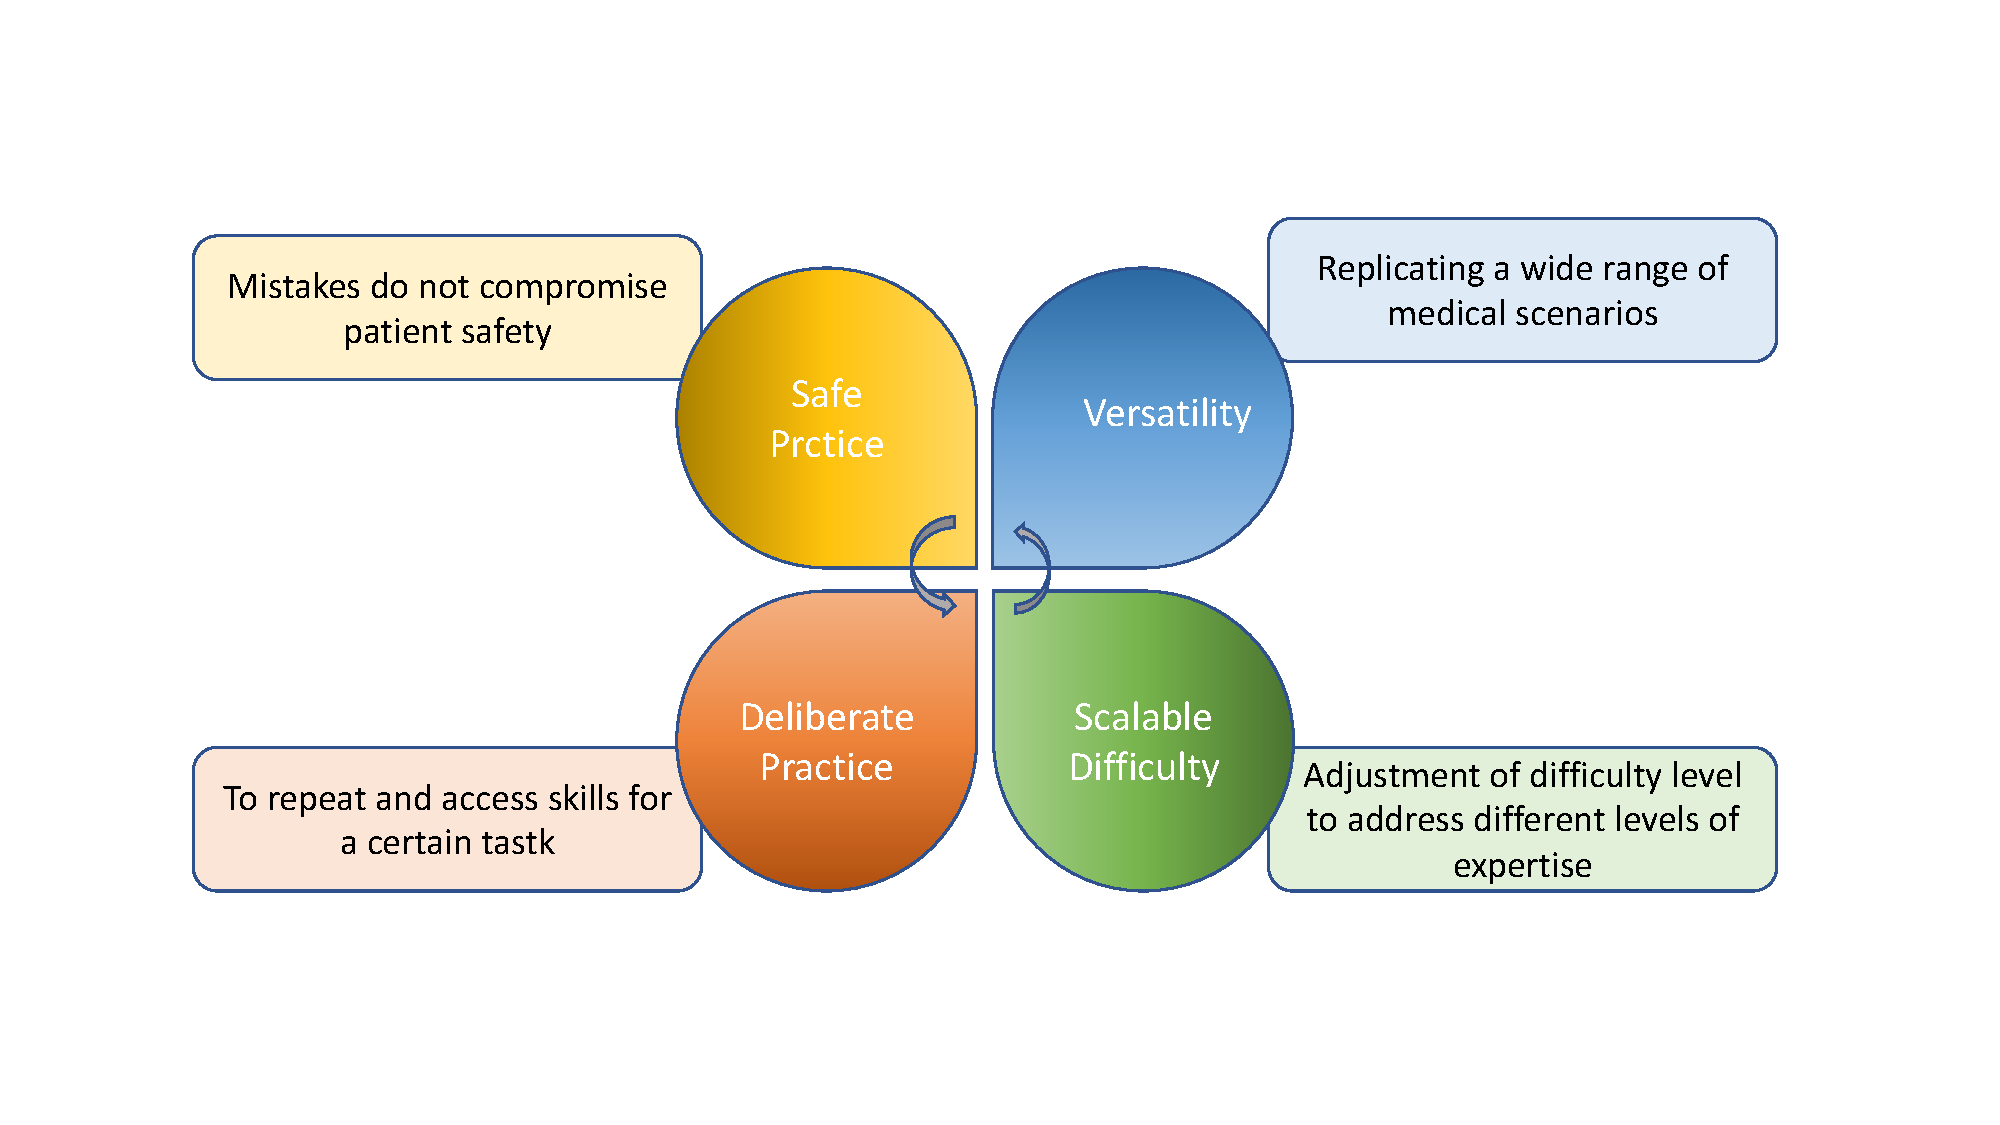
\includegraphics[width=1.0\textwidth]{./pics/computer_simulation}
	\end{tabular}
	\caption{\footnotesize Different factors affecting computer-based medical simulation.} \label{fig: ch1f1}
\end{figure}

The PAD can be abstracted as a fluid-structural interaction problem and be described by fluid and structure mathematic equations, respectively.  The two most popular approaches for solving FSI problems are monolithic method and partitioned method. For the monolithic approach, the two sets of equations, fluid and structural, are solved simultaneously. The mutual influence of each other can be considered directly. The obvious advantage of this scheme is simplicity. Only one global matrix is needed so that both the fluid and structural parts can be solved within the same space discretization and time marching scheme. On the contrary, we lose the flexibility to precisely control each partition. The other approach is partitioned method. The two sets of equations are solved separately and pass boundary conditions to each other like a cycle. The solution of fluid equations is calculated while the structural part is waiting for new input and vice versa. A coupling algorithm to exchange the interaction solution between two phases as a pair of modules. The Implicit-Explicit (IMEX) Runge-Kutta (RK) time integration approach has been proved the accuracy and efficiency on coupling the high order schemes\cite{zhang2016high}.

The high order parallel fluid solver \cite{liang2007large, liang2007large, liang2009effect} is accomplished and a series of CFD studies has been conducted along the ideal geometries. To implement the more realistic simulation, the tissue of blood vessel wall shall be considered as elastic material. Therefore, an accurate and efficient solver for elasticity equation is needed. The solver should be capable on calculating the material behavior according to the stiffness property, which is the response of the deformable model reacting to the external forces. The simplest model is mass-spring model which is easy to compute but can not accurately determine the material behavior. The other approach is finite element method, which is based on the continuum mechanics, has gained popularity since the results are more reliable. On the contrary to the mass-spring model, the FEM can specify the stiffness of the model by only using a few characteristic parameters, such as Young's modulus, Poisson ratio and the geometries. However, the challenges for FEM is very difficult to be used in real-time application due to the very high computational expense. 

\begin{figure}[H]
	\centering
	\begin{tabular}{c}
		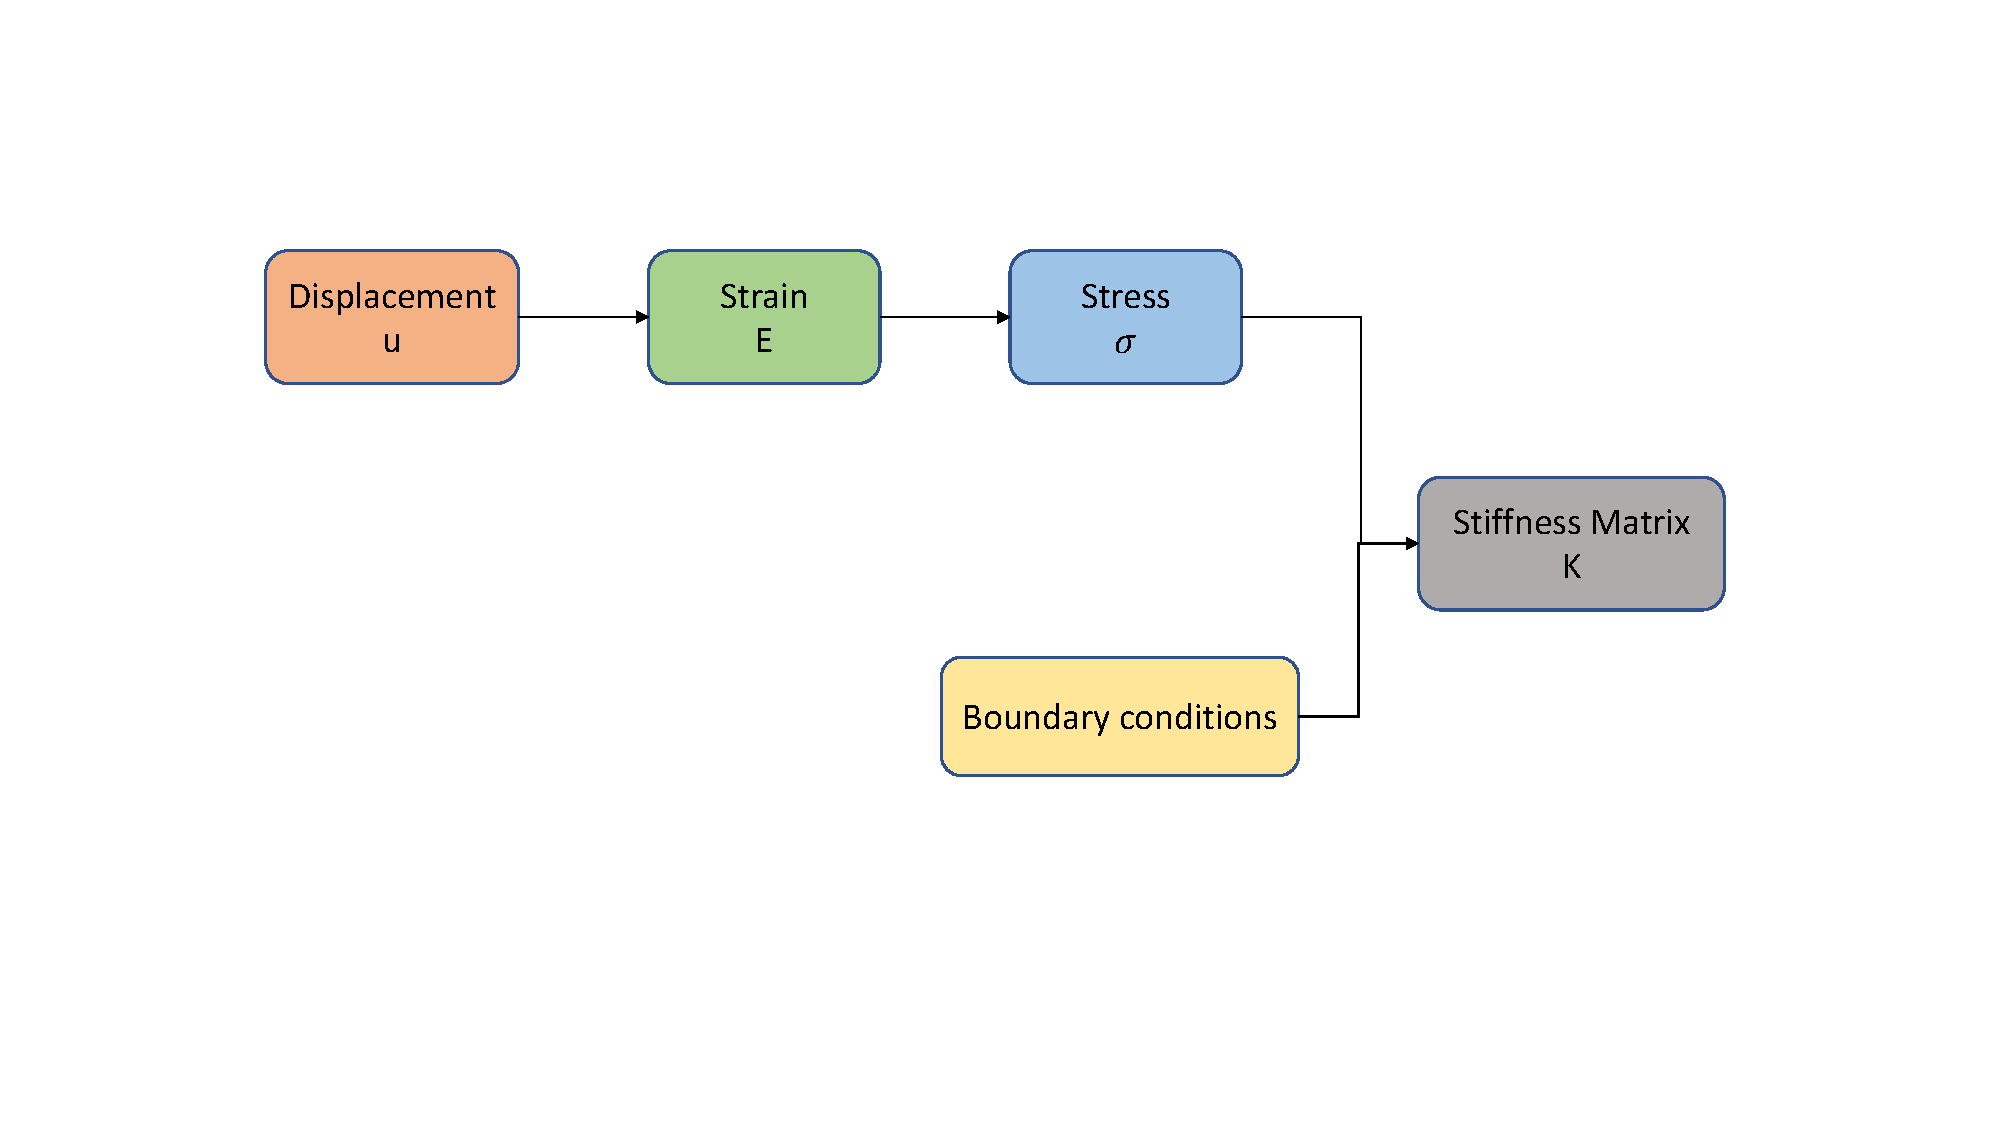
\includegraphics[width=1.0\textwidth]{./pics/construct_matrix}
	\end{tabular}
	\caption{\footnotesize Construct stiffness matrix.} \label{fig: ch1f2}
\end{figure}

Fig \ref{fig: ch1f2} shows a general process of calculating the stiffness matrix for a deformable material object. The stiffness matrix is derived from the gradient of stress which is calculated by the displacement and material property. The boundary conditions are imposed upon the contact interaction.

\begin{figure}[H]
	\centering
	\begin{tabular}{c}
		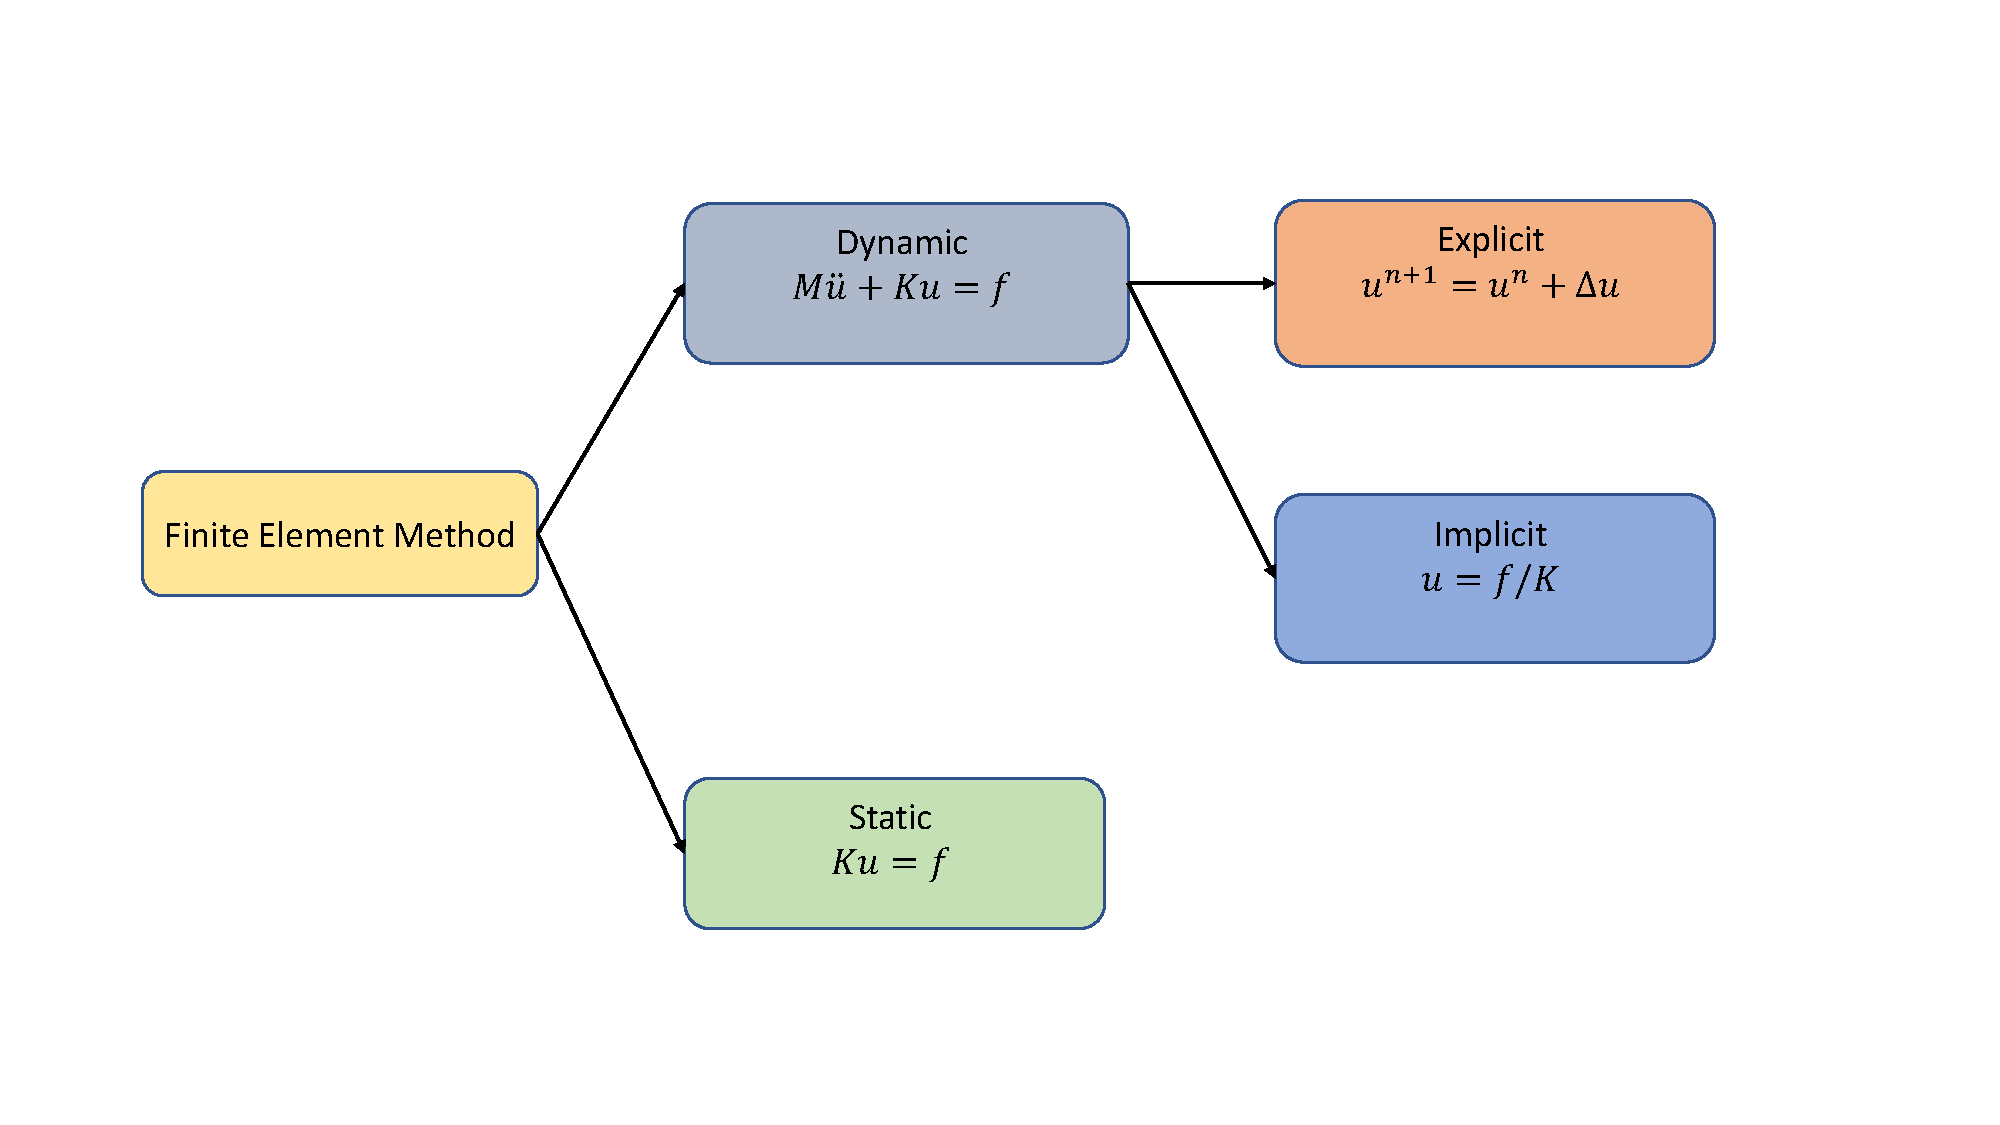
\includegraphics[width=1.0\textwidth]{./pics/fem}
	\end{tabular}
	\caption{\footnotesize Static and dynamic finite element method.} \label{fig: ch1f3}
\end{figure}

The Fig \ref{fig: ch1f3} displays both static analysis and dynamic analysis for a set of linear system of elasticity equations. The steady-state and transient finite element problem are studied with static analysis and dynamic analysis respectively. The latter is time dependent. In dynamic analysis, we shall consider the spatial discretization by using both explicit and implicit time integration schemes\cite{bathe2008finite}. The implicit time marching scheme is computationally costly, since the matrix inversion for large linear system is required every time-step, similar to solving the static problem. The benefit is unconditionally stable for large time step. On the other hand, the explicit time marching scheme requires much lower computational cost as no linear solver is involved for each time-step. However, the size of each time step has to satisfy the numerical stability criteria. 


The linear system of elasticity equations derived from the FEM method is positive definite and too large to be direct inverse. The most time consuming part in the FEM analysis in Fig \ref{fig: ch1f2} is solving the linear system. The complex system can be simplified as a matrix form $ \mathbf{A} \mathbf{x} = \mathbf{b} $. To sovle it, there are two main group of algorithms, directive method and iterative method. Considering the better performance on memory usage and computing time, the iterative method gains more affirmatives\cite{brussino1989comparison} for large scale problems. Preconditioned Conjugate Gradient (PCG) is the one of the most popular method because of its robustness and fast speed. However, Due to the PCG requires positive definite matrix. It is still very challenging to implement finite element analysis using implicit scheme to study the material real-time response behavior. Therefore, the domain decomposition method combined with parallel computing scheme is one emerging choice to tackle that problem.

Parallel computing requires extra effort to tailor the algorithm to achieve concurrent execution. The challenges to reach that purpose include learning and understanding programming paradigms, design the balance load to maximize the usage of bandwidth, minimize the overhead on data communication and synchronization to avoid potential data race problems. In a short conclusion, the high performance computation based on CPU clusters is very challenging dealing with the complex hardware architecture and associated distributed memory. n that case, some modern techniques such as MPI, Intel Math-Kernel library and LAPACK-BLAS can assist us to achieve optimal scalability. The key point for accomplish promising performance is to reduce the overhead latency by employing large number of active processors and ensure the balance of loads on each processor.

\subsection{Numerical Method Review}

The Weak Galerkin Finite Element Method (WG-FEM)is a novel developed, effective numerical method for solving partial differential equations. The WG method is first developed by Dr. Junping Wang and Xiu Ye in 2011, and applied on solving second order elliptic equation\cite{wang2014weak}. The main theory of WG method is to introduce a series of weak operators such as weak gradient, weak divergence and weak curl on the computation of corresponding forms of differential equations. The WG finite element method provides a  brand new perspective to solve numerical problems. It builds up the classic Continuous Galerkin(CG) method to an advanced stage. The WG method can be applied on variety of partial differential equations include second order elliptical equation, elasticity equation\cite{wang2016locking}, Stokes equations \cite{wang2016weak} and Maxwell's equations \cite{mu2013weak}, etc. The WG method inherits the discontinuity from the discontinuous basis functions. The construction of discrete matrix is independent with any external coefficients. The interior unknown variables can be eliminated to the boundary unknown variables to construct a linear system which only consists by degree of freedom(DOFs) along the element boundary. In short, even though the total DOFs of WG method is larger than Discontinuous Galerkin method (DG), the interior unknown variables can eliminated through Schur complement method. The only left DOFs are along the element boundary which are far less than DOFs in DG finite element method. The elemental stiffness matrix of WG method can be constructed upon each element, which is consistent with CG FEM method. 

%-----------------------------------------------------
\section{Objectives of this Work}

The CG FEM analysis of continuum mechanics is widely used to study and predict the material deformation. The results are generally accurate and reliable for analyzing the relationship between load and deformation. However, the computational complexity and cost inhibits the application on conquering the real-time FSI problems. Massive parallel computing is required for obtaining large linear system. In this work, we investigate methods for efficient parallel scheme which enables high-order novel finite element method in solving elasticity equation.

We employ the WG-FEM to convert the bilinear form equations into a positive definite linear system. The WG method has the capacity on varying high-order elements. The selection of polynomials on interior or boundary region is flexible which enhance the freedom on computational simulation. Moreover, the discontinuity features in the WG method which empowers the parallel computation capability.

The Balancing Domain Decomposition by Constraints (BDDC) method is an ideal candidate for entitling the massive parallel capacity to WG-FEM. BDDC identifies the two spaces (primal and dual) to divide and conquer the original computational domain. By minimizing the global communication and synchronization overhead,  WG-BDDC enriches the scalability of elasticity equations as a superlinear speedup curve.

The main objective of this dissertation is to deliver high speed, accuracy and scalability in WG-BDDC based analysis. Fig \ref{fig: ch1p4} shows the paths to accomplish the objectives in this work. The results of the research significantly improves the computation of the elastic material response, including in clinic judgment and other medical applications.

\begin{figure}[H]
	\centering
	\begin{tabular}{c}
		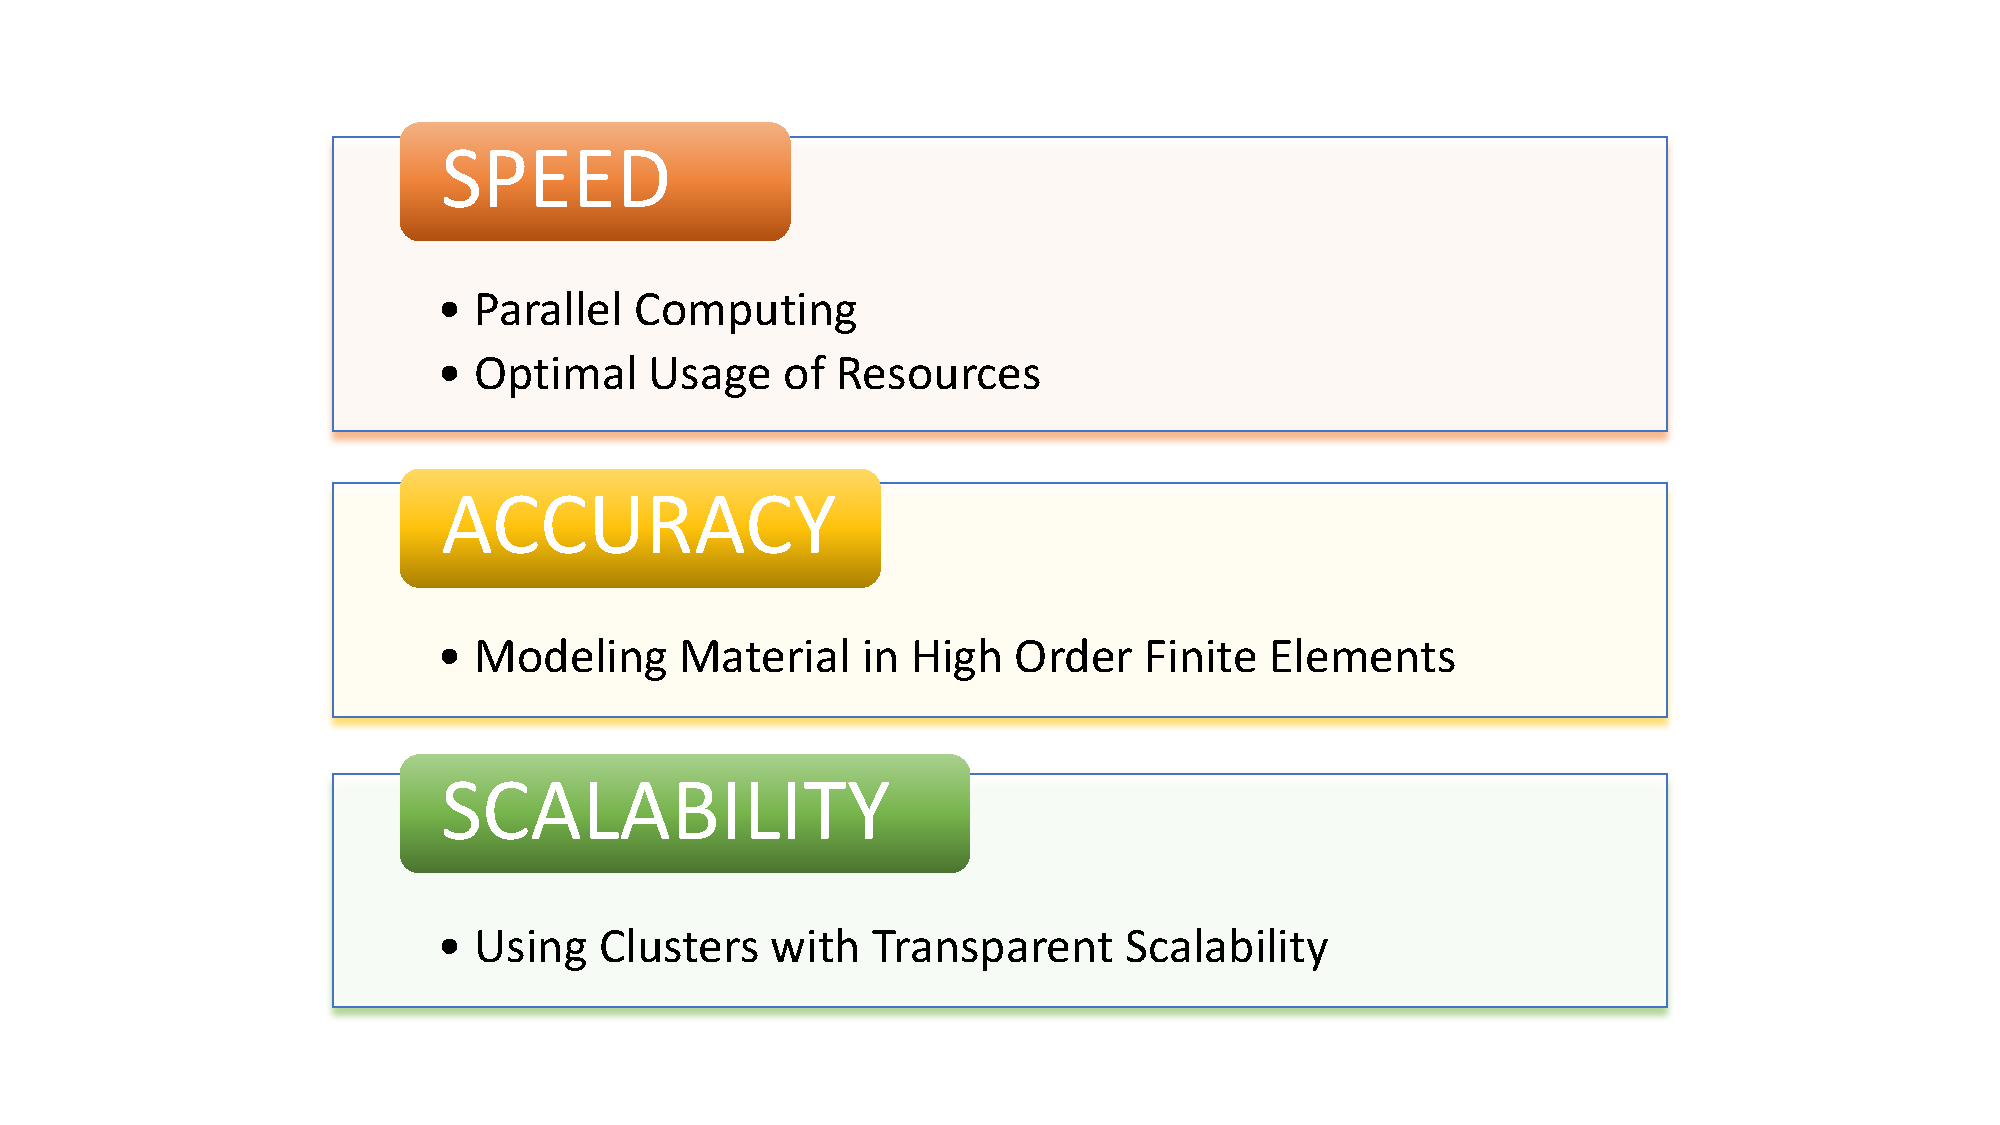
\includegraphics[width=1.0\textwidth]{./pics/ch1p4}
	\end{tabular}
	\caption{\footnotesize Objectives and methodology.} \label{fig: ch1p4}
\end{figure}

To validate the WG-BDDC scheme and develop the software, we first design the hybrid WG-CG element. The results are consistent with the benchmark of CG only element so the fidelity is proved. Then we extend the WG element to BDDC method and verify the properties of convergence and the order of accuracy with parallel fashion. Finally, the scalability is discussed under the parallel computing framework.

The rest of this dissertation is organized as :

\begin{itemize}
	\item Chapter 2 presents the background and basics of WG method.
	\item Chapter 3 discusses the hybrid WG-CG element the performance on nonlinear elasticity equation.
	\item Chapter 4 introduces the WG-BDDC method for second order elliptic and elasticity equation.
	\item Chapter 5 shows the study of effect multiple stenoses on the peripheral artery diseases.
	\item Chapter 6 concludes this work and outlook the future work.
\end{itemize}


\chapter{Numerical Method}
\label{chapter2}

%--------------------------------------
\section{Mathematical Models and Numerical Method}
\label{sec:equations}

\subsection{Linear Elastic Equation and Weak Galerkin Method}
Consider an elastic body subject to an exterior force $ \mathbf{f} $, we denote the computational domain as $ \Omega $ and its continuous boundary as $ \Gamma = \partial \Omega $. The governing equation for linear elasticity can be written as

\begin{equation}
\nabla \cdot \sigma(\mathbf{u}) = \mathbf{f}, \qquad in \quad \Omega 
\end{equation}
\begin{equation}
\mathbf{u} = \hat{\mathbf{u}}, \qquad on \quad \Gamma
\end{equation}
where $ \sigma(\mathbf{u}) $ is the symmetric Cauchy stress tensor. For linear, isotropic and homogeneous materials, the stress-strain relation is
\begin{equation}
\sigma(\mathbf{u}) = 2 \mu \varepsilon(\mathbf{u}) + \lambda (\nabla \cdot \mathbf{u}) \mathbf{I}
\end{equation}
where $ \varepsilon(\mathbf{u}) = \frac{1}{2} (\nabla \mathbf{u} + \nabla \mathbf{u}^{T}) $, $ \mu $ and $ \lambda  $ are Lame indices which can be written as 
\begin{equation}
\lambda = \frac{E\mu }{(1 + \mu) (1 - 2\mu)}
\end{equation}
\begin{equation}
\mu = \frac{E}{2(1+\mu)}
\end{equation}
where $ E $ is the elasticity modulus and $ \mu $ is the Poisson's ratio.



The weak function on the domain is $ \mathbf{u} = \{\mathbf{u}_0, \mathbf{u}_b \}, \quad \mathbf{u}_0 \in L^{2} (T) $. The first function $ \mathbf{u}_0 $  represents the interior domain of the function $ \mathbf{u} $ . The second function $ \mathbf{u}_b $ represents the value of function $ \mathbf{u} $ on the boundary of domain $ T $ . The key notion is that for two function $ \mathbf{u}_0 $  and $ \mathbf{u}_b $  are independent with each other along . The weak function is defined as
\begin{equation}
V_{h} = \{ \mathbf{v} = \{ \mathbf{v}_0, \mathbf{v}_b \} : \mathbf{v}_0 \in P_{j} (T^0), \mathbf{v}_b \in P_{l}(e), e \subset \partial T\}
\end{equation}

The key of the weak Galerkin method is to approximate the solution in the weak discrete space $ S(T) $. The discrete weak gradient $ \nabla_{w} \mathbf{u} \in [P_{r} (T)]^{d} $ for $ \mathbf{u} \in V_{h} $ on each element $ T $:
\begin{equation}
(\nabla_w \mathbf{u}, \mathbf{q})_{T} = - (\mathbf{u}_0, \nabla \cdot \mathbf{q})_{T} + \langle \mathbf{u}_b, q \cdot \mathbf{n} \rangle_{\partial T}
\end{equation}

For the discrete weak divergence, $ \nabla_{w} \cdot \mathbf{u} \in [P_{r} (T)]^{d} $ is defined
\begin{equation}
(\nabla_w \cdot \mathbf{u}, \mathbf{q})_{T} = - (\mathbf{u}_0, \nabla  \mathbf{q})_{T} + \langle \mathbf{u}_b \cdot \mathbf{n}, q  \rangle_{\partial T}
\end{equation}

Then we can define the weak strain tensor by using the weak gradient
\begin{equation}
\varepsilon_{w} (\mathbf{u})  = \frac{1}{2} (\nabla_w  \mathbf{u} + \nabla_w  \mathbf{u}^T)
\end{equation}

Analogously, we can define the weak stress tensor as
\begin{equation}
\sigma_{w} ( \mathbf{u}) = 2 \mu \varepsilon_{w} ( \mathbf{u}) + \lambda (\nabla_w \cdot  \mathbf{u}) \mathbf{I}
\end{equation}

The bilinear form of governing equation of continuous Galerkin method is following
\begin{equation}
a( \mathbf{u},  \mathbf{v}) = ( \mathbf{f},  \mathbf{v})
\end{equation}

The above approximation function $  \mathbf{u} $ and gradient $ \nabla \mathbf{u} $ is not well defined for the discontinuous feature of weak Galerkin method, the new form is 
\begin{equation}
a( \mathbf{u}_w,  \mathbf{v}_w) + s( \mathbf{u},  \mathbf{v}) = ( \mathbf{f},  \mathbf{u})
\end{equation}
the term $ s( \mathbf{u},  \mathbf{v}) $ is a stabilizer enforcing a weak continuity which measures the discontinuity of the finite element solution. The governing equation in weak form can be introduced by two bilinear equations
\begin{equation}
s( \mathbf{u},  \mathbf{u}) = \sum_{T\in \Omega}^{N} h_{T}^{-1} \langle Q_{b}  \mathbf{u}_0 -  \mathbf{u}_b, Q_b  \mathbf{v}_0 -  \mathbf{v}_b \rangle_{\partial T}
\end{equation}
where $ Q_b $ is the projection from the interior unknown variables to boundary unknown variables. Commonly it is taken as $ 1 $. The discrete bilinear equation has the assemblage form
\begin{equation}
a( \mathbf{u}_w,  \mathbf{u}_w) = \sum_{T \in \Omega}^{N} 2(\mu \varepsilon_w ( \mathbf{u}), \varepsilon_w ( \mathbf{v}))_T + \sum_{T \in \Omega}^{N}(\lambda \nabla \cdot \mathbf{u}, \nabla_w \cdot \mathbf{v})_T
\end{equation}


%--------------------------------------
\section{Existing Numerical Methods Review}
In this section, we present and analyze several most widely used numerical method to solve finite element problems. The details of each method are presented in the following subsections. 
\subsection{Classic Continuous Galerkin Finite Element Method}
Finite element method is an efficient solution to solve partial differential equations. The core idea is to convert the original partial differential equation to a equivalent bilinear form weak function. Then we partition the computational domain into polygon meshes. In each mesh element, we construct the finite element space. Then the bilinear form is discretized into a summation of finite elemental spaces. The solution is approximated based on the calculation of assembled matrix. More details can be found in \cite{zienkiewicz1977finite, ciarlet2002finite, hughes2012finite, reddy1993introduction}

\subsection{Discontinuous Galerkin Finite Element Method}


\subsection{Mixed Finite Element Method}



%---------------------------
\section{Weak Galerkin Finite Element Methods}
\subsection{Weak Galerkin triangular meshes}

Consider triangular element linear type basis function for both interior and boundary subspaces $ P_{1}(T) / P_{1} (\partial T) $
\begin{equation}
\phi_{k} = \{ \lambda_{k}, 0 \}, \qquad k = 1,2, 3
\end{equation}
\begin{equation}
\phi_{3 + l} = \{ 0, \mu_{l} \}, \qquad l = 1, 2, \cdots , 2N
\end{equation}
where N is the number of element boundaries.

\begin{figure}[h]
	\centering
	\begin{tabular}{c}
		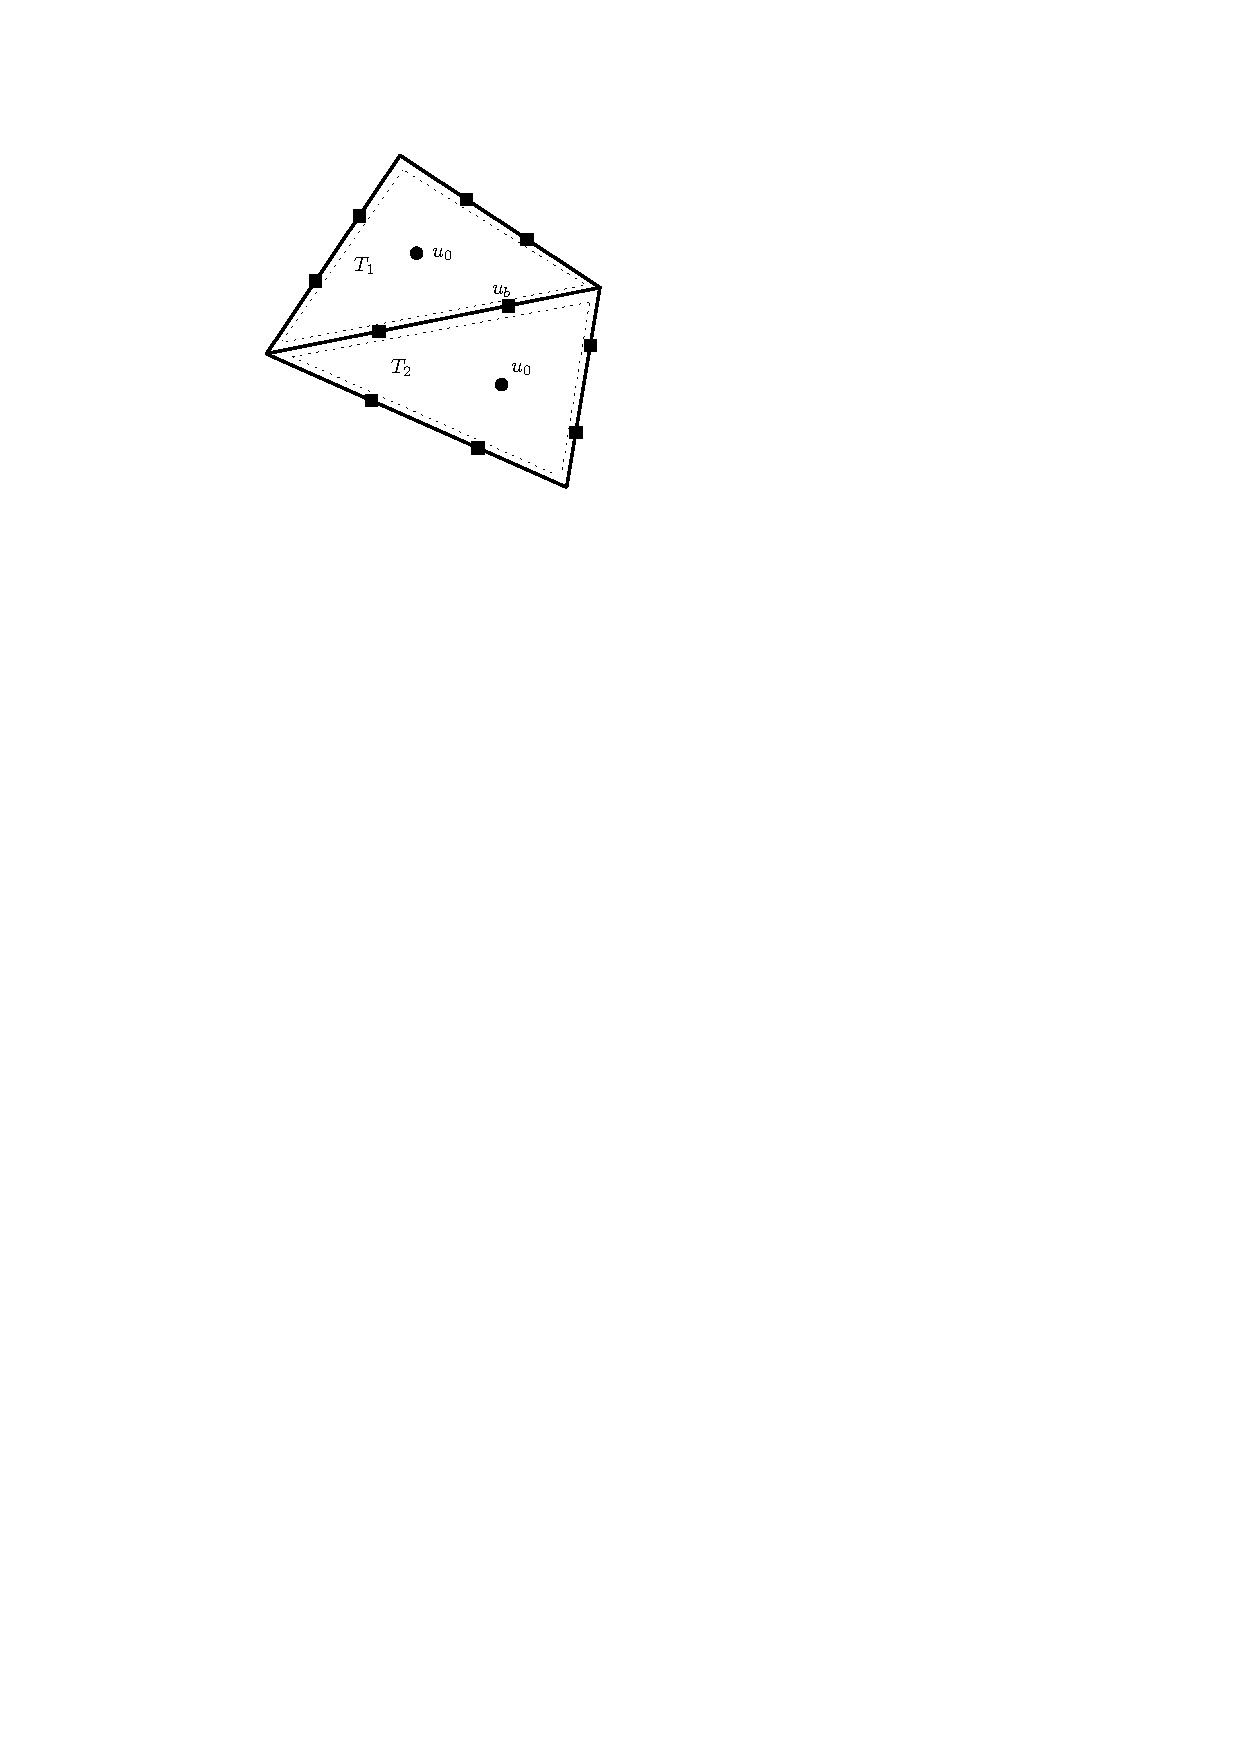
\includegraphics[width=0.5\textwidth]{./pics/triangle.pdf}
	\end{tabular}
	\caption{\footnotesize Weak Galerkin triangular elements and solution points.}\label{fig1: triangle}
\end{figure}

\subsection{Weak Galerkin quadrilateral meshes}

Consider triangular element linear type basis function for both interior and boundary subspaces $ Q_{1}(T) / Q_{1} (\partial T) $
\begin{equation}
\phi_{k} = \{ \lambda_{k}, 0 \}, \qquad k = 1,2, 3
\end{equation}
\begin{equation}
\phi_{3 + l} = \{ 0, \mu_{l} \}, \qquad l = 1, 2, \cdots , 2N
\end{equation}
where N is the number of element boundaries.
\begin{figure}[h]
	\centering
	\begin{tabular}{c}
		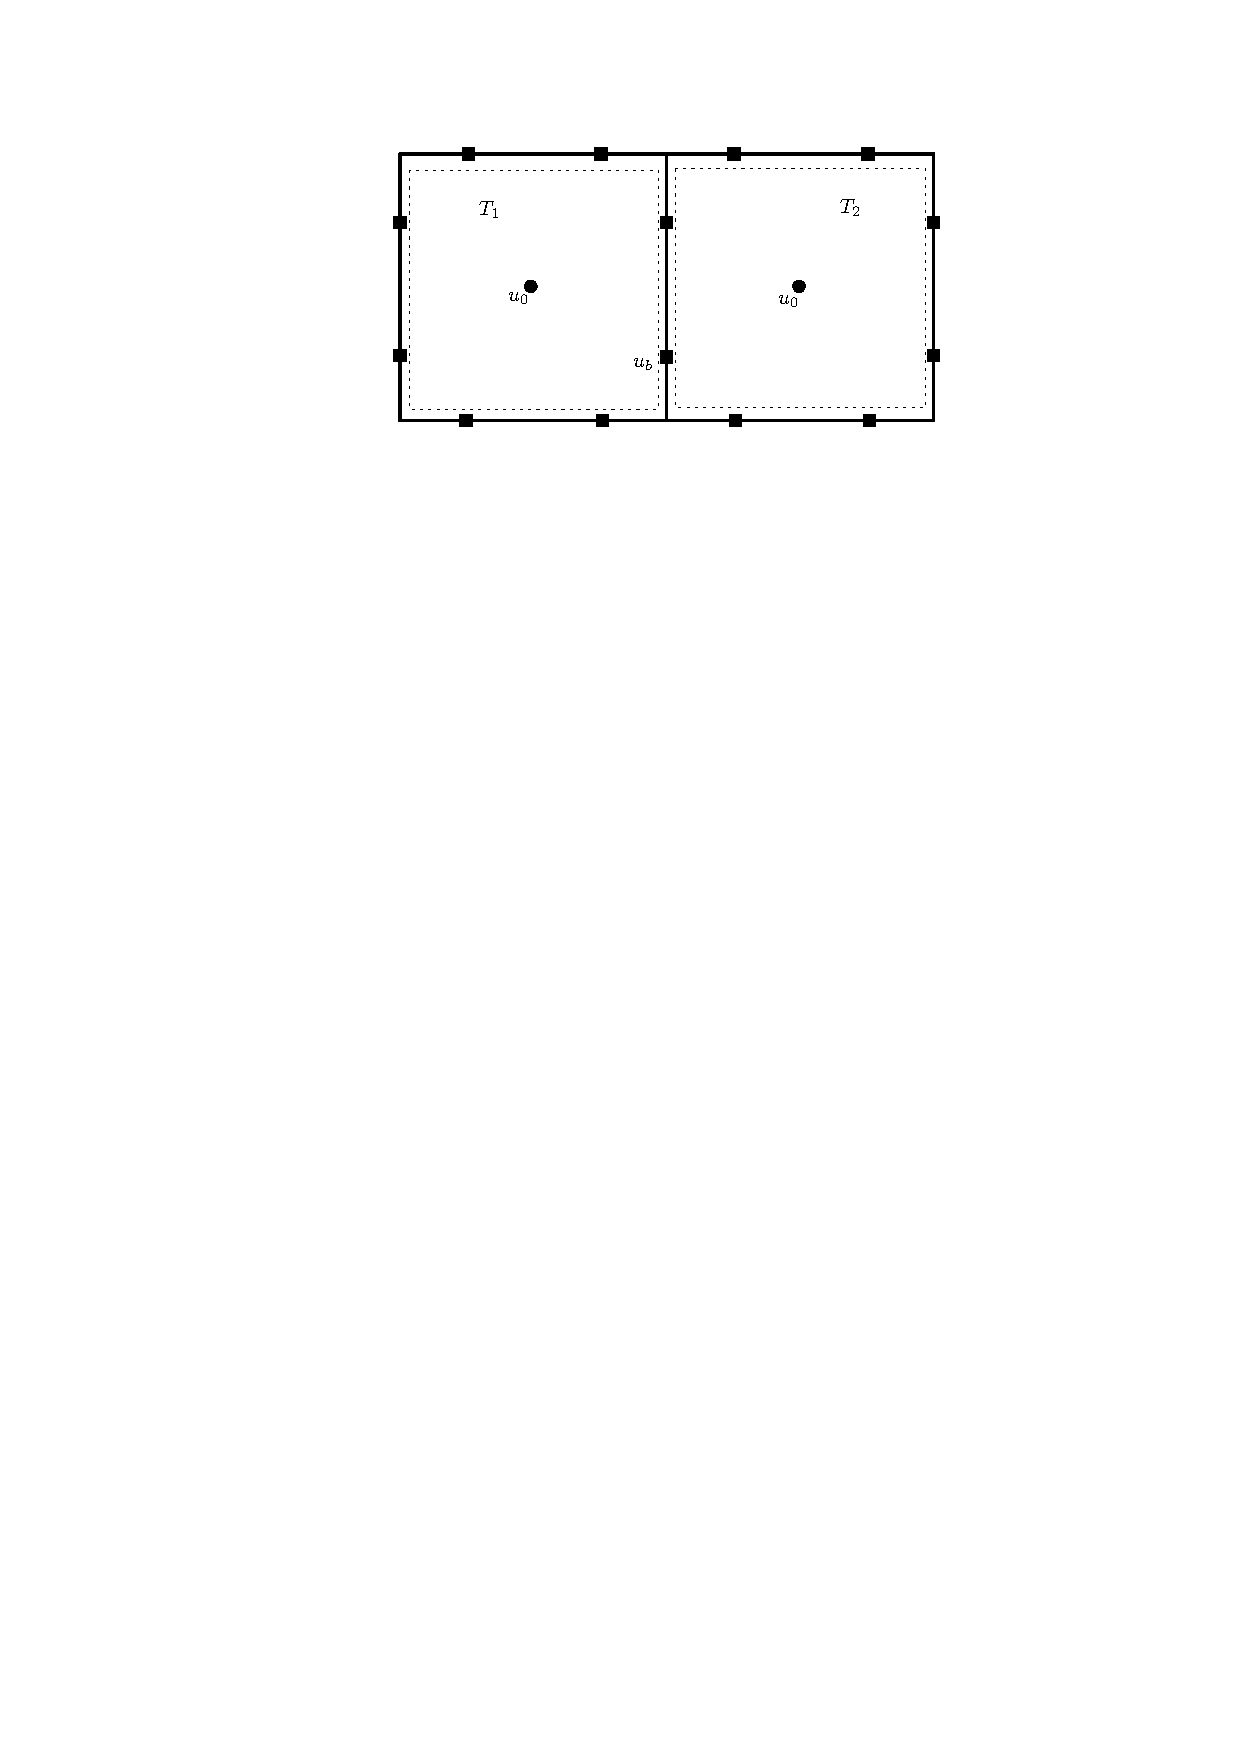
\includegraphics[width=0.8\textwidth]{./pics/quad.pdf}
	\end{tabular}
	\caption{\footnotesize Weak Galerkin quadrilateral elements and solution points.}\label{fig2: quad}
\end{figure}

%--------------------------


\chapter{Hybrid Weak Galerkin - Continuous Galerkin Finite Element Method}
\label{chapter3}

In this chapter, we present a novel parallel computing method to effectively solve linear and nonlinear elasticity equations. The WG finite element method is newly developed by Dr. Junping Wang and Dr. Xiu Ye  \cite{wang2013weak}. We develop a novel hybrid element which combines the elements of both WG and CG finite element. The new hybrid element inherits the discontinuous feature of the WG method. To create a hybrid element, we treat the WG element as cargo ship and the CG element as the container. We insert multiple CG elements in one single WG element. 

The hybrid element takes advantages from both the WG and the CG element. For the WG element, it is discontinuous and can be calculated as a non-overlapping subdomain without extra unknown variables, such as Lagrangian multiplier. For the CG element, it's simple to construct and compute. The hybrid element use WG element as the subdomain boundary interface and CG and interior refine elements.

Like the standard FEM, the WG method can be used to solve generic partial differential equations. An advanced feature of the WG finite element method is that the entire problem can be decomposed into multiple local problems. In these local problems, the differential operators are approximated and reconstructed by small-size matrices. The WG method provides optimal orders of accuracy in spatial discretization for difficult problems on serial computers. However, the performance of the WG method on parallel computers has not yet been examined.

This chapter is organized as following. We first introduce the weak Galerkin method and the derivations of the bilinear form of nonlinear elasticity equation. Then we discuss the details of matrix construction. An improved stabilizer is designed for implementing time marching schemes. For the numerical method, we present the details of the parallel scheme including the explicit Central Difference method and the implicit time marching scheme, the Newmark-Beta method \cite{adeli1978algorithms}. At the end of this chapter, we present the numerical results of one-dimensional linear and nonlinear elastic equation. The second order accuracy are achieved with observed superlinear speedup.

\section{Nonlinear Elasticity Equation}

Consider an elastic body subject to an exterior force $ \mathbf{f} $, we denote the computational domain as $ \Omega $ and its continuous boundary as $ \Gamma = \partial \Omega $. The governing equation for elasticity can be written as
\begin{equation}
-\nabla \cdot \boldsymbol{\sigma(u)} = \mathbf{f}, \quad in \quad \Omega
\end{equation}
\begin{equation}
\mathbf{u} = \hat{\mathbf{u}},  \qquad on \quad \Gamma
\end{equation}
where $ \boldsymbol{\sigma(u)} $ is Cauchy stress. For isotropic and homogeneous materials, the stress-strain relation is
\begin{equation}
\boldsymbol{\sigma(u)} = 2\mu \varepsilon(\mathbf{u}) + \lambda (\nabla \cdot \mathbf{u}) \mathbf{I}
\end{equation}
the $ \mu $ and $ \lambda $ are Lame indices which can be written as
\begin{equation}
\lambda = \frac{E\nu}{(1 + \nu)(1 - 2\nu)}
\end{equation}
where $ E $ is the elasticity modulus and $ \nu $ is Poisson's ratio. 

The geometric nonlinear strain-displacement relation can be written as following format
\begin{equation}
\boldsymbol{\varepsilon(u)}= \frac{1}{2} (\nabla u + \nabla u^{T} - (\nabla u^{T}) \cdot \nabla u)
\end{equation}

The weak function on domain is $ u = \{u_0, u_b\} $, $ u_{0} \in L^{2} (T)$. The first function $ u_0 $ represents the interior domain of the function $ u $. The second function $ u_{b} $ represents the boundary value of function $ u $. The key notion is that for two functions $ u_0 $ and $ u_{b} $ are independent with each other. The weak function is defined as 
\begin{equation}
U_{h} = \{ u = \{u_{0}, u_{b} \}: u_{0} \in P_{j} (T^{0}), u_{b} \in P_{l} (e), e \subset \partial T \}
\end{equation}

The key of the weak Galerkin method is to approximate the solution in weak discrete space $ S(T) $. The discrete weak gradient $ \nabla_{w} u \in [P_{r} (T)]^{d} $ for $ u \in V_{h} $ on each element $ T $:

\begin{equation}
(\nabla_{w}, q)_{T} = -(u_{0}, \nabla \cdot q)_{T} + \langle u_{b}, q \cdot \mathbf{n} \rangle_{\partial T}
\end{equation}

for the discrete weak divergence, $ \nabla_{w} \cdot \mathbf{u} in [P_{r} (T)]^{d} $ is defined 
\begin{equation}
(\nabla_w \cdot u, q)_{T} = -(u_{0}, \nabla q)_{T} + \langle u_{b} \cdot \mathbf{n}, q \rangle_{\partial T}
\end{equation}

Then we can define the weak linear strain tensor by using the weak gradient
\begin{equation}
\varepsilon_{w} (u) = \frac{1}{2} (\nabla_{w} u + \nabla_{w} u^{T})
\end{equation}

Analogously, the nonlinear weak strain tensor is defined by 
\begin{equation}
\varepsilon_{w} (u) = \frac{1}{2} (\nabla_{w} u + \nabla_{w} u^{T} + (\nabla_w u^{T}) \cdot \nabla_w u ) 
\end{equation}

The weak stress can be defined as
\begin{equation}
\sigma_{w} (u) = 2 \mu \epsilon_{w}(u) + \lambda(\nabla_{w} \cdot u) \mathbf{I}
\end{equation}

The weak form of governing equation of continuous Galerkin method as
\begin{equation}
a(\mathbf{u}, \mathbf{v}) = (\mathbf{f}, \mathbf{v})
\end{equation}
the above approximation function $ v $ and the gradient $ \nabla v $ is not well defined for the discontinuous feature of weak Galerkin method. The new form is 
\begin{equation}
a(\mathbf{u}_{w}, \mathbf{v}_{w}) + s(\mathbf{u}, \mathbf{v}) = (\mathbf{f}, \mathbf{v})
\end{equation}
the term $ s(\mathbf{u}, \mathbf{v}) $ is a stabilizer enforcing a weak continuity which measures the discontinuity of the finite element solution. The governing equation in weak form can be introduced by two bilinear equations
\begin{equation}
s(\mathbf{u}, \mathbf{v}) = \sum_{T\in \Omega}^{N} h_{T}^{-1} \langle Q_{b} u_{0} - u_{b}, Q_{b} v_{0} - b_{b} \rangle_{\partial T}
\end{equation}
where $ Q_{b} $ is the projection parameter defined by the interior and boundary value. $ h_{T} $ is the characteristic length of mesh element. It is a constant number which usually is taken as 1.

The governing equation has the weak form as
\begin{equation}
a(\mathbf{u}_{w}, \mathbf{v}_{w}) = \sum_{T \in \Omega}^{N} 2(\mu \varepsilon_w (u), \varepsilon_{w} (v))_{T} + \lambda(\nabla_{w} \cdot \mathbf{u}, \nabla_{w} \cdot \mathbf{v})_{T}
\end{equation}

\section{Hybrid WG-CG Element}

In this section, we introduce the design of hybrid element, the construction of the basis functions. The one dimensional WG element has the shape function
\begin{equation}
\phi_{0}^{1} = \frac{x - x_{i +1}}{x_{i} - x_{i +1}}, \quad \phi_{b}^{1} = 1
\end{equation}

\begin{equation}
\phi_{0}^{2} = \frac{x - x_{i}}{x_{i + 1} - x_{i}}, \quad \phi_{b}^{2} = 1
\end{equation}

\begin{figure}[H]
	\centering
	\begin{tabular}{c}
		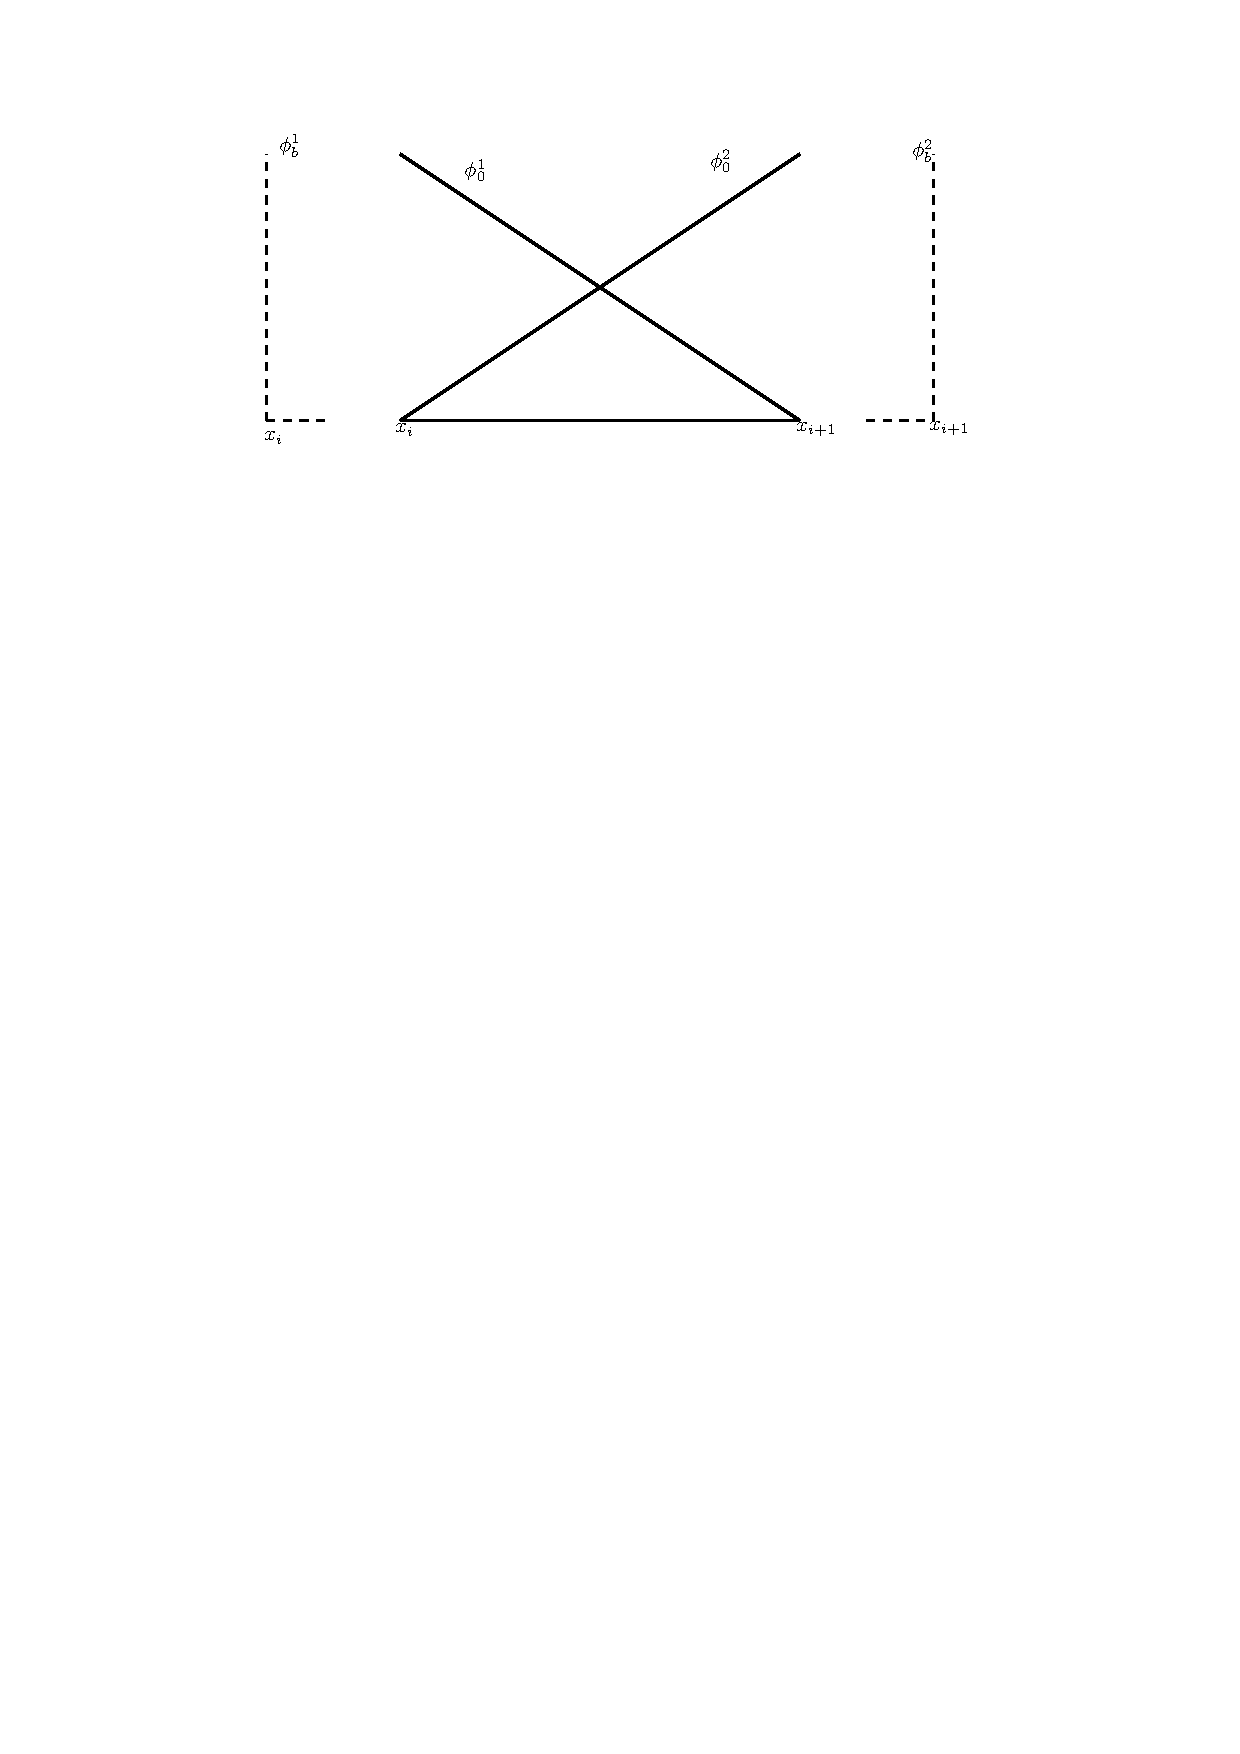
\includegraphics[width=0.7\textwidth]{./pics/oneD}
	\end{tabular}
	\caption{\footnotesize Basis function of one dimensional weak Galerkin element}
\end{figure}

Based on the weak gradient function, the boundary basis functions are independent of the interior basis functions, Therefore, we can insert an arbitrary number of CG element basis functions into the WG element. Each weak Galerkin element is considered as one sub-element that neighbored with adjacent elements. The interior CG elements are corrected by the coarse mesh which is the WG element. The boundary basis function of WG element is shared by adjacent elements and constitute the coarse mesh. The newly designed basis function of hybrid element can be illustrated as

\begin{figure}[h]
	\centering
	\begin{tabular}{c}
		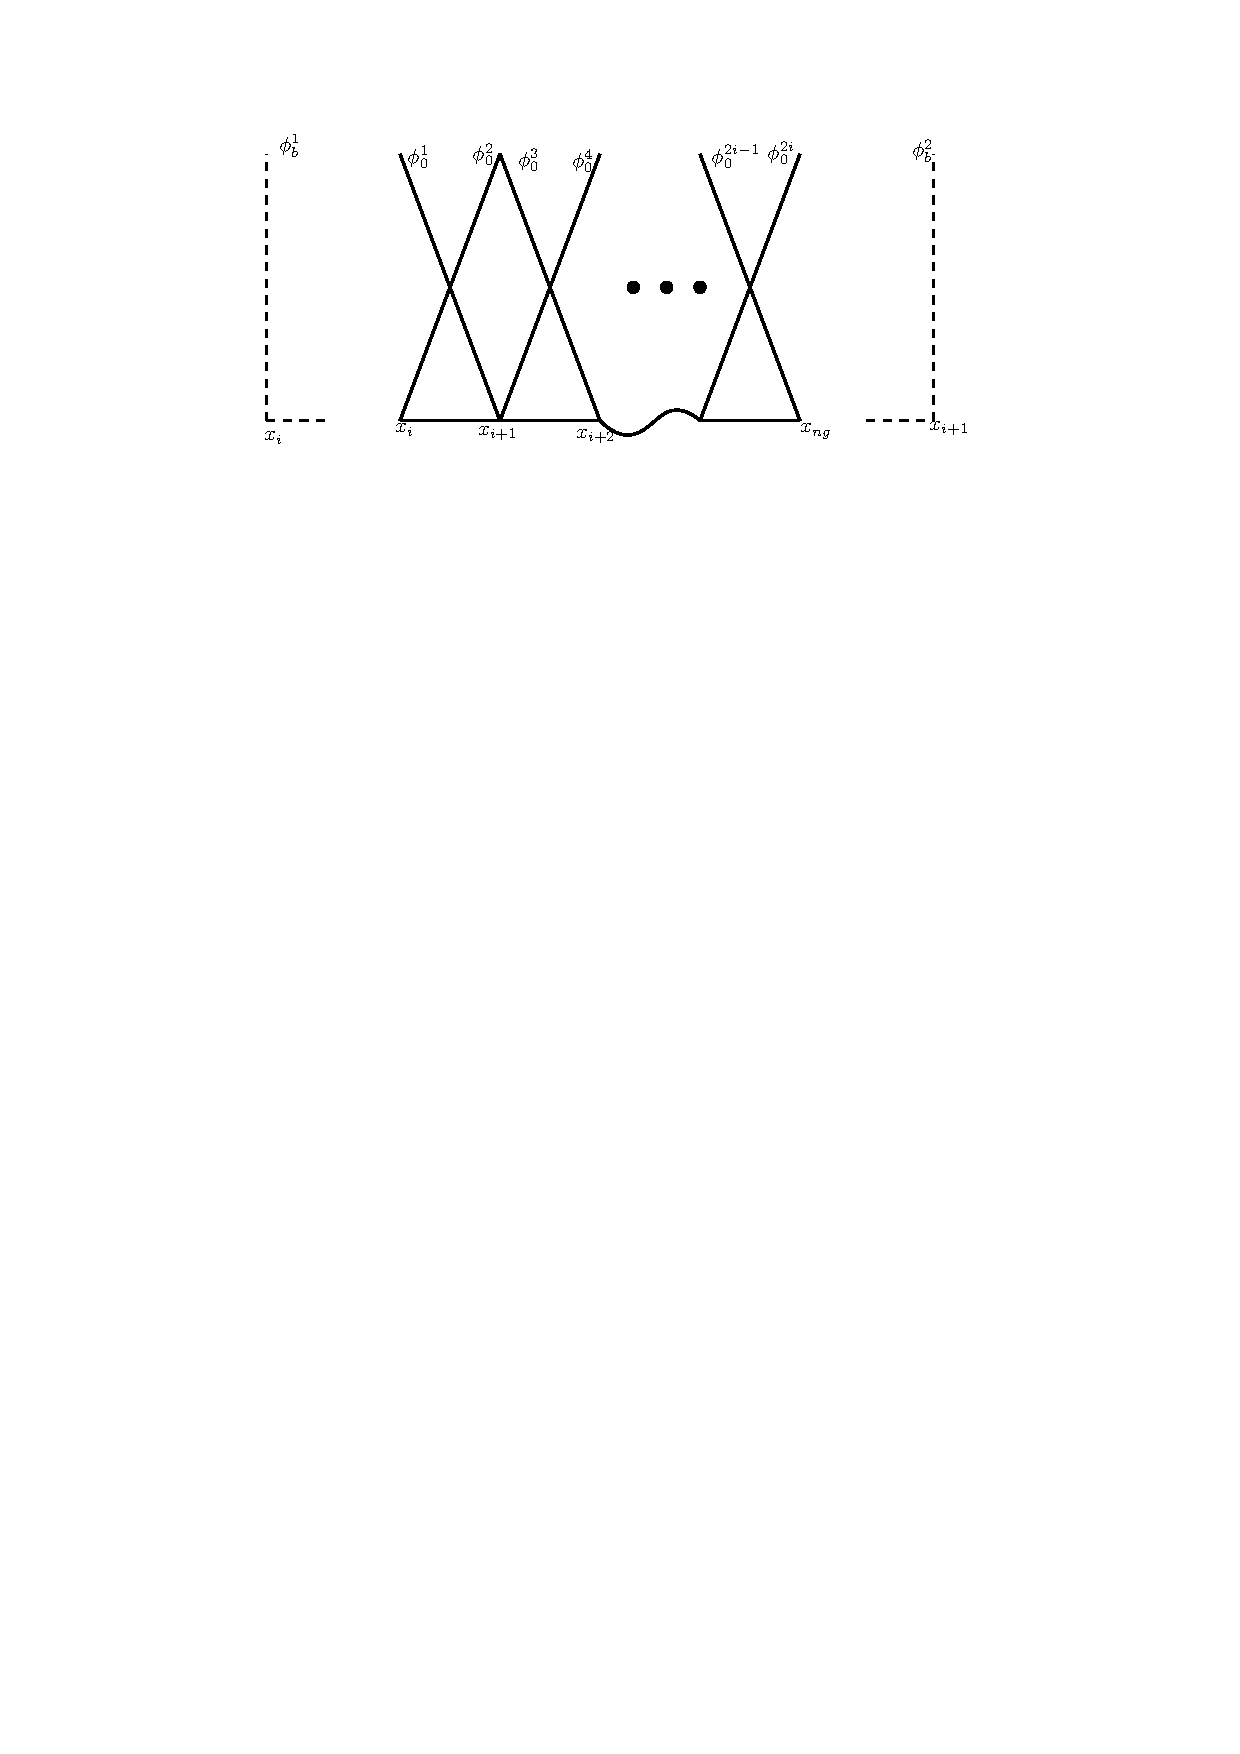
\includegraphics[width=0.7\textwidth]{./pics/hybrid}
	\end{tabular}
	\caption{\footnotesize Basis function of hybrid WG-CG element, an arbitrary number of CG elements are inserted into WG element}
\end{figure}

As above figure, in one WG element, there are multiple CG element basis functions. All the interior basis functions are linear and shared the same boundary basis functions of WG element. This is the illustration of the hybrid element basis functions.

\section{The Improved Stabilizer}

\subsection{Deficiency of Original Stabilizer}

Here we present the parallel computing scheme for one dimensional linear and nonlinear elastic equations. The governing equation for dynamic equation is 
\begin{equation}
M\ddot{u} + Ku = f
\end{equation}

In the hybrid elements, the information of mass is missing for the corresponding boundary values. The original governing equation in matrix form is
\begin{equation} \label{eq:incomp}
\begin{bmatrix}
M_{00} & 0 \\0 & 0 \\
\end{bmatrix}\begin{bmatrix}
\ddot{u}_{0} \\ \ddot{u}_{b} \\
\end{bmatrix} + \begin{bmatrix}
K_{00} & K_{0b} \\ K_{b0} & K_{bb} \\
\end{bmatrix} \begin{bmatrix}
u_{0} \\ u_{b} \\
\end{bmatrix} = \begin{bmatrix}
f_{0} \\ 0 \\
\end{bmatrix}
\end{equation}

from above equation we can find that the mass matrix for $ \ddot{u}_{b} $ is not complete. The information of mass is missing on the boundary basis functions. Under this circumstance, the explicit time marching scheme is unable to initiate. 


\subsection{Improvement}
To avoid the deficit of time marching scheme, we introduce a newly designed stabilizer, namely, the generic stabilizer.
\begin{equation}
s(\mathbf{u}, \mathbf{v}) = \sum_{T \in \Omega}^{N} h_{T}^{-1} \langle Q_{b} \ddot{u}_{0} - \ddot{u}_{b}, Q_{b} v_{0} - v_{b} \rangle_{\partial T}
\end{equation}

Consider the Central difference method as 
\begin{equation} \label{eq:cd}
\frac{\partial^{2} u}{\partial^{2} t} = \frac{u^{n + 1} - 2 u ^{n} + u^{n - 1}}{(\Delta t)^{2}}
\end{equation}

For one stabilizer matrix $ h^{-1} \langle Q_{b} \ddot{u} - \ddot{u}_{b}, Q_{b} v_{0} - v_{b} \rangle $, we apply Eq. \eqref{eq:cd} on it and rewrite it as
\begin{equation}
\langle  h^{-1} \frac{Q_{b} (u^{n + 1}_{0} - 2 u ^{n}_{0} + u_{0}^{n - 1})}{(\Delta t)^{2}}, Q_{b} v_{0} - v_{b} \rangle - h^{-1} \langle \frac{u_{b}^{n + 1} - 2u_{b}^{n} + u_{b}^{n - 1}}{(\Delta t)^{2}} , Q_{b} v_{0} - v_{b} \rangle
\end{equation}

Then we calculate the boundary integral and write the result in matrix form $ S $. The stabilizer is written in
\begin{equation}
\frac{h^{-1}}{(\Delta t)^{2}} \langle Q_{b} u_{0}^{n + 1} - u_{b}^{n + 1} , Q_{b} v_{0}- v_{b} \rangle - \frac{2h^{-1}}{(\Delta t)^{2}} \langle Q_{b} u_{0}^{n} - u_{b}^{n} , Q_{b} v_{0}- v_{b} \rangle + \frac{h^{-1}}{(\Delta t)^{2}} \langle Q_{b} u_{0}^{n - 1} - u_{b}^{n - 1} , Q_{b} v_{0}- v_{b} \rangle 
\end{equation}


\begin{equation}
\frac{h^{-1}}{(\Delta t)^{2}} \begin{pmatrix}
\begin{bmatrix}
S_{00} & S_{0b} \\ S_{b0} & S_{bb} 
\end{bmatrix} \cdot 
\begin{bmatrix}
u_{0}^{n + 1} \\ u_{b}^{n + 1}
\end{bmatrix}
 - 2\begin{bmatrix}
S_{00} & S_{0b} \\ S_{b0} & S_{bb}
\end{bmatrix} \cdot
\begin{bmatrix}
u_{0}^{n} \\ u_{b}^{n}
\end{bmatrix} + 
\begin{bmatrix}
S_{00} & S_{0b} \\ S_{b0} & S_{bb} 
\end{bmatrix} \cdot
\begin{bmatrix}
u_{0}^{n - 1} \\ u_{b}^{n - 1}
\end{bmatrix}
\end{pmatrix}
\end{equation}

We combine the discretized stabilizer with the incomplete equation Eq. \eqref{eq:incomp}, we can construct the governing equation in a new matrix form
\begin{eqnarray} \label{eq:newForm}
&& h^{-1}\begin{bmatrix}
M_{00} + S_{00} & S_{0b} \\ S_{b0} & S_{bb}
\end{bmatrix} \cdot \begin{bmatrix}
u_{0}^{n + 1} \\ u_{b}^{n + 1}
\end{bmatrix} + (\Delta t)^{2} 
\begin{bmatrix}
K_{00} & K_{0b} \\ K_{b0} & K_{bb}
\end{bmatrix} \cdot \begin{bmatrix}
u_{0}^{n + 1} \\ u_{b}^{n + 1}
\end{bmatrix}\\
& =& 2 h^{-1} \begin{bmatrix}
S_{00} & S_{0b} \\ S_{b0} & S_{bb}
\end{bmatrix} \cdot
\begin{bmatrix}
u_{0}^{n} \\ u_{b}^{n}
\end{bmatrix} - h^{-1}\begin{bmatrix}
S_{00} & S_{0b} \\ S_{b0} & S_{bb}
\end{bmatrix} \cdot
\begin{bmatrix}
u_{0}^{n - 1} \\ u_{b}^{n - 1}
\end{bmatrix} + (\Delta t)^{2} \begin{bmatrix}
f_{0} \\ 0
\end{bmatrix}
\end{eqnarray}

In Eq. \eqref{eq:newForm}, the mass matrix has completed with $ M_{bb} = S_{bb} $ information for boundary unknown variables. In the time marching scheme, the $ M_{bb}^{-1} $ produces valid result.

The original stabilizer requires that the values in the equation must be the same category. We extend the rule to all the unknown variables in the bilinear form. After the injection of the new stabilizer, the above equation becomes

\begin{equation}
\begin{bmatrix}
M_{00} & 0 \\ 0 & M_{bb}
\end{bmatrix}\begin{bmatrix}
\ddot{u}_{0} \\ \ddot{u}_{b}
\end{bmatrix} + \begin{bmatrix}
K_{00} & K_{0b} \\
K_{b0} & K_{bb} 
\end{bmatrix} \begin{bmatrix}
u_{0} \\ u_{b}
\end{bmatrix} = \begin{bmatrix}
f_{0} \\ 0
\end{bmatrix}
\end{equation}

Consequently, both explicit and implicit time marching scheme can be implemented on above matrices.

\subsection{Parallel Computing Method}

For both linear and nonlinear equations, we implement the implicit time marching scheme, the Newmark-Beta method. It has the following steps

\begin{equation}
\ddot{u}_{0}^{n+1} = \frac{(u_{0}^{n+1} - \tilde{u}_{0})}{\beta \Delta t^{2}}
\end{equation}
\begin{equation}
\ddot{u}_{b}^{n+1} = \frac{(u_{b}^{n+1} - \tilde{u}_{b})}{\beta \Delta t^{2}}
\end{equation}

The $ \tilde{u} $ represents the intermediate step, then we can use it to calculate the value of next step

\begin{equation}
\tilde{u}_{0} = u_{0}^{n} + \dot{u}_{0}^{n} \Delta t + \frac{1}{2} \Delta t^{2} \ddot{u}_{0}^{n} (1 - 2 \beta)
\end{equation}

\begin{equation}
\tilde{u}_{b} = u_{b}^{n} + \dot{u}_{b}^{n} \Delta t + \frac{1}{2} \Delta t^{2} \ddot{u}_{b}^{n} (1 - 2 \beta)
\end{equation}

To reduce the local unknown variable $ u_{0} $ into a smaller size global matrix of unknown variable $ u_{b} $, we apply the Schur complement method. The correlation between interior unknown variables and boundary variables is following equation

\begin{equation}
u_{0}^{n+1} = -K_{00}^{-1} K_{0b} u_{b}^{n+1} + K_{00}^{-1} g_{1}
\end{equation}

Therefore, the original large sparse global matrix is transformed into a small condensed global matrix with the only one set of unknown variables, $ u_{b} $. The governing equation has the new form
\begin{equation}
u_{b}^{n+1} = [K_{b0}(-K_{00}^{-1}K_{0b}) + K_{bb}]^{-1} (g_{2} - K_{b0} (K_{00}^{-1} g_{1}))
\end{equation}

Then we can simplify the above equation into
\begin{equation}
u_{b}^{n+1} = K^{'} f^{'}
\end{equation}

From above equations, the boundary unknown variable $ u_{b} $ is updated. In each time step, we convert local unknown variable $ u_{0} $ to $ u_{b} $ through local Schur complement method to reduce the computational cost. After condensing the matrix, we can calculate the solution by matrix inversion. 

\subsection{The Parallel Computing Work Flow}

For one-dimensional elastic equation, the original governing equation can be converted to a sparse tri-diagonal stiffness matrix to a blocked decomposed submatrices

 \begin{figure}[H]
 	\centering
 	\begin{tabular}{c}
 		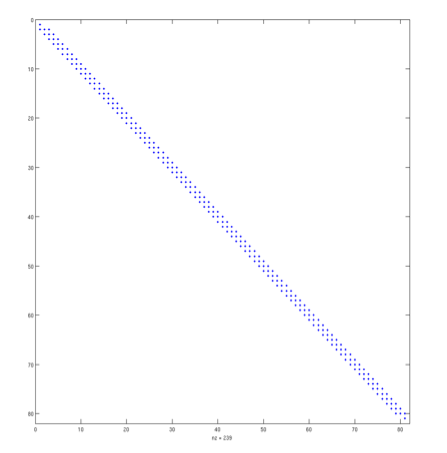
\includegraphics[width=0.5\textwidth]{./pics/matrix1.png}
 	\end{tabular}
 	\caption{\footnotesize Global sparse tri-diagonal stiffness matrix}
 \end{figure}
 
 For the WG element, the global matrix is constructed as above figure. The elements are continuously arranged. The parallel computing scheme such as Schur complement method cannot be directly applied. An external loading vector like Lagrangian multiplier is required. Our hybrid WG-CG element method is discontinuous, it will provide a discontinuous matrix form as below figure. 
 
  \begin{figure}[H]
  	\centering
  	\begin{tabular}{c}
  		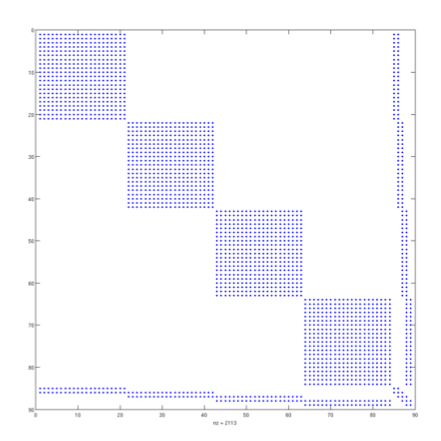
\includegraphics[width=0.5\textwidth]{./pics/hmatrix1.png}
  	\end{tabular}
  	\caption{\footnotesize Blocked stiffness matrix after domain decomposition}
  \end{figure}
  
  The original large sparse stiffness matrix is compressed in a very small matrix on the right bottom corner by using Schur complement method. In another word, the main computational load is split into the calculation of square matrices. Each square matrix represents the interior unknown variables in one single hybrid element. The size of hybrid element is determined by the number of interior CG elements since the boundary basis function remains the same. The entire computational domain is decomposed into multiple subdomains and each subdomain corresponds to one single processor. After the global calculation, the interior unknown variables can be recovered through local computing.
  
  The parallel computing work flow chart is described as following
  
    \begin{figure}[h]
    	\centering
    	\begin{tabular}{c}
    		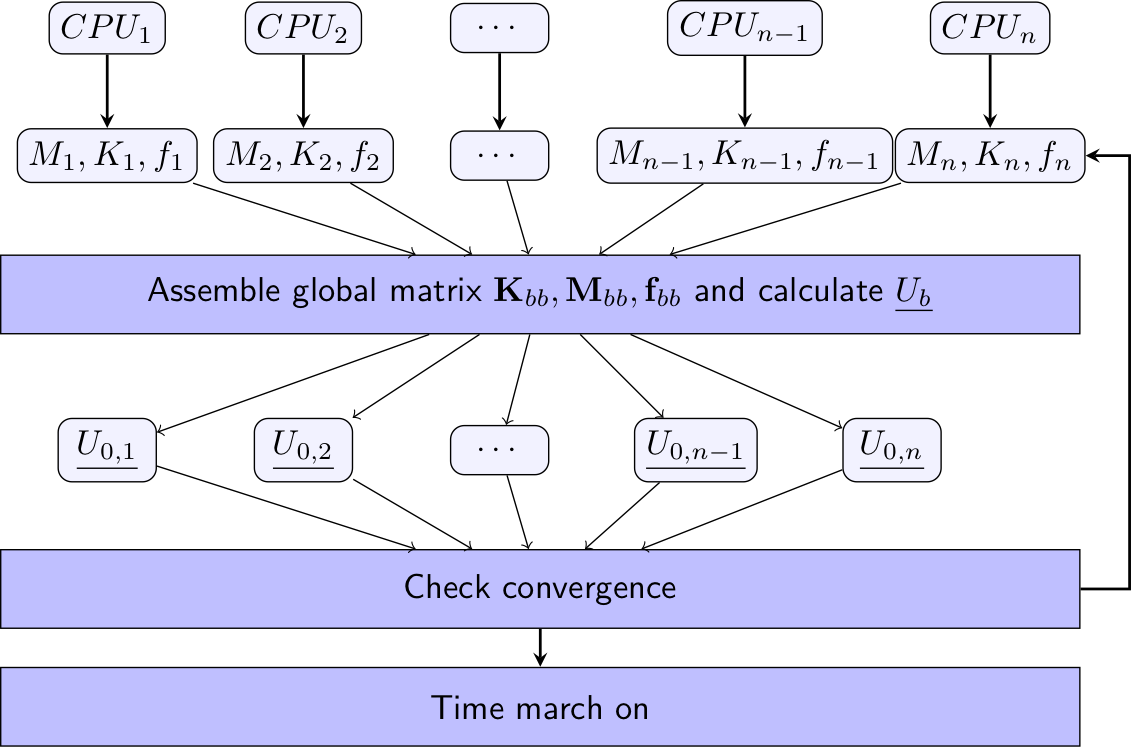
\includegraphics[width=0.6\textwidth]{./pics/flowchart1.png}
    	\end{tabular}
    	\caption{\footnotesize Parallel computing workflow chart for WG-CG method}
    \end{figure}
    
   \begin{enumerate}
   	\item Each CPU reads in preprocessed file and initiates MPI communication\cite{gropp1996high}.
   	\item Every hybrid element is dealt by each individual processor. Local stiffness matrices and load vectors are constructed on parallel machine.
   	\item The global stiffness boundary matrix is assembled additively. The global boundary unknown variables are obtained and passed to each processor through MPI communication.
   	\item Once the global residual is less than the tolerant value, current Newmark-Beta time iteration complete and move to the next time step.
   \end{enumerate}
   
   To accelerate the performance, we use the open source library such as LAPACK/BLAS to calculate the computationally expensive operators in terms of the block Cholesky elimination, matrix multiplication and vector operations. This implementation largely benefits the programming process and works very well among different high performance computing platforms.
   
   The software has been tested on the George Washington University super computing cluster, ColonialOne, with Xeon E5-2650v2 2.6GHz 8-core processors with 128 GB of RAM each.
   
   \section{Numerical Results}
   
   \subsection{Geometric linear elastic equation}
   
   We design a numerical test to verify the hybrid element with analytical solution $ u = sin (2 \pi x) $. In each WG element, we set 20 CG elements and then observe the accuracy of $ u_0 $, $ u_b $ and the effect of stabilizer.
   
      \begin{figure}[H]
      	\centering
      	\begin{tabular}{c}
      		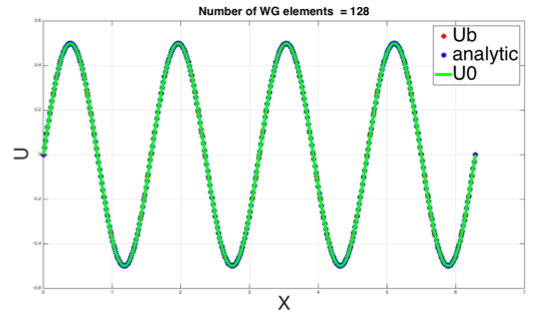
\includegraphics[width=0.8\textwidth]{./pics/result1d1.png}
      	\end{tabular}
      	\caption{\footnotesize Linear elastic equation results for hybrid WG-CG element}
      \end{figure}
      
      \begin{table}[h]
      	\setlength{\tabcolsep}{2pt} {
      		\caption{ Error and accuracy of hybrid WG-CG element for linear elasticity.}
      		\label{Tab:hwgcg l1}
      		\vspace{-5pt}
      		\begin{center}
      			%	\scalebox{0.6}{
      			\begin{tabular}{c|c|c|c|c}
      				\hline
      				\multicolumn{5}{c}{\# CG = 20} \\
      				\hline
      				\#WG & $ E (u_{0}) $ & $ O(u_{0}) $ & $ E(u_{b})  $& $ O(u_{b})  $\\
      				\hline
      				$ 16 $ & $ 1.7636e-4 $ & - & $ 3.8909e-4 $ & - \\
      				\hline
      				$ 32 $ & $ 4.4745e-5 $ & $ 1.98 $& $ 9.8515e-5 $ & $ 1.99 $ \\
      				\hline
      				$ 64 $ & $ 1.1271e-5 $ & $ 1.99 $ & $ 2.4744e-5 $ & $ 1.99 $ \\
      				\hline
      				$ 128 $ & $ 2.8286e-6 $ & $ 1.99 $ & $ 6.1941e-6 $ & $ 2.00 $\\
      				\hline
      			\end{tabular}
      			%	}
      		\end{center} }
      	\end{table}
      	
      	The above table demonstrates the accuracy of the hybrid element on linear elasticity equation by using central difference time marching scheme.
      	With the increasing of the number of hybrid WG-CG elements, we observed a second order accuracy of both interior and boundary unknown variables. This test shows that the hybrid element has the excellent compatibility for linear elastic equation.
      	
      	To explore the capability in dynamic problem using time marching schemes, we extend the test case with the same analytic solution. By implementing the generic stabilizer above, both explicit and implicit time marching scheme are ready to test. For explicit time marching scheme, we choose the forward Euler method \cite{jameson1991time} and define the relative small time step to fit the critical time marching step \cite{cundall1979discrete}. For the implicit scheme, we choose the Newmark-Beta method \cite{hahn1991modified}. For every test case, a constant loading force is applied on the right-hand side as a Neumann boundary condition \cite{ng1999fast}. Meanwhile, we fix the left-hand side as Dirichlet boundary condition. The results are shown as following charts
      	
      	      \begin{figure}[H]
      	      	\centering
      	      	\begin{tabular}{c}
      	      		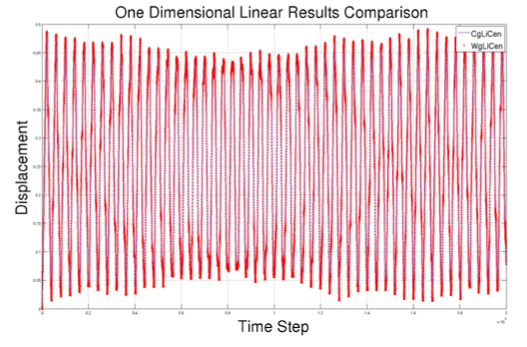
\includegraphics[width=0.8\textwidth]{./pics/result1d2.png}
      	      	\end{tabular}
      	      	\caption{\footnotesize The results comparison between CG only and hybrid WG-CG element for explicit scheme}
      	      \end{figure}
      	      
      	       \begin{figure}[H]
      	       	\centering
      	       	\begin{tabular}{c}
      	       		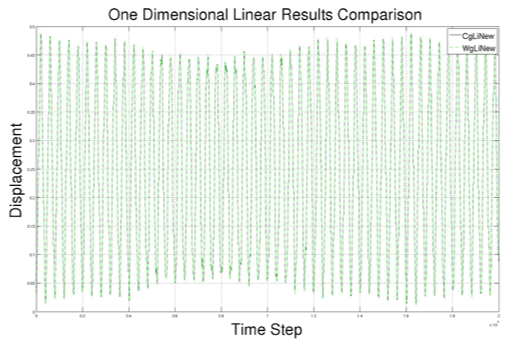
\includegraphics[width=0.8\textwidth]{./pics/result1d3.png}
      	       	\end{tabular}
      	       	\caption{\footnotesize The results comparison between CG only and hybrid WG-CG element for implicit scheme}
      	       \end{figure}
      	       
      	       The above two figures illustrates the comparison of deflections. We compare the solutions between our hybrid WG-CG element and classic CG element. In both implicit and explicit time marching scheme, the average difference between two methods is less than $ 10^{-5} $. Based on the results, our hybrid WG-CG solver shows optimal convergence to the established CG solver. The lower error value encouraged us to extend the hybrid element to handle geometric nonlinear problems.
      	       
 \subsection{Geometric nonlinear elasticity equation}
 
 Both the large deflection and body rotation require the nonlinear strain-displacement relation. We test the performance of accuracy and efficiency of hybrid WG-CG element. We continue using the classic CG element solver as the reference and compare our new method to the reliable existing solutions.
 
 By following the linear elastic equation test cases, we load constant force as the boundary condition and compare the solutions between the serial CG solver and parallel implicit hybrid WG-CG solver. We divide the entire computational domain into 20 subdomains. In another word, each subdomain corresponds to an individual hybrid WG-CG element. In each hybrid element, we insert 20 standard CG elements. Each processor handles one hybrid element and the communicates with each other through MPI library. 
 
 The CG solver choose 400 standard linear CG elements to maintain the same resolution. We track the deflection on the right tip of the domain and plot the two sets of solutions in the same figure to compare the difference as following
 
  \begin{figure}[H]
  	\centering
  	\begin{tabular}{c}
  		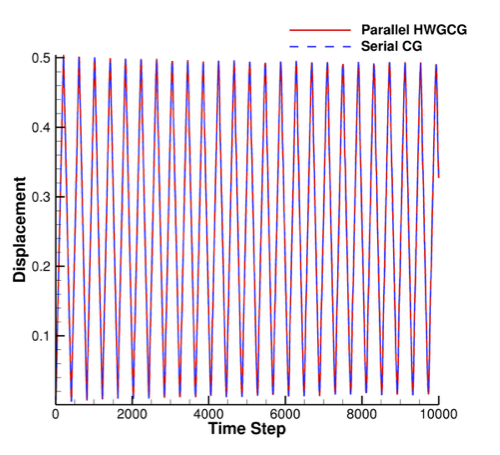
\includegraphics[width=0.8\textwidth]{./pics/result1d4.png}
  	\end{tabular}
  	\caption{\footnotesize The results comparison between CG only and hybrid WG-CG element by using parallel implicit scheme with constant boundary condition}
  \end{figure}
  
  An optimal convergence of the two independent solutions shows an excellent accuracy of the parallel hybrid solver. The average difference is less than $ 10^{-4} $, which is same as the previous linear test.
  
  To verify the the robustness of the new solver, a periodic boundary condition is enforced to substitute the constant variable where $ f = sin (2 \pi t) $. The comparing results is as following chart
  
    \begin{figure}[H]
    	\centering
    	\begin{tabular}{c}
    		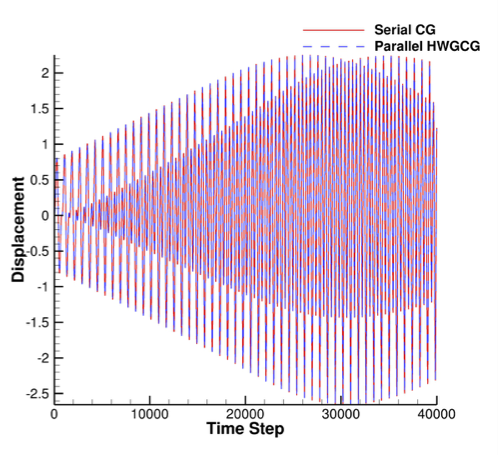
\includegraphics[width=0.8\textwidth]{./pics/result1d5.png}
    	\end{tabular}
    	\caption{\footnotesize The results comparison between CG only and hybrid WG-CG element by using parallel implicit scheme with periodic boundary condition}
    \end{figure}
    
    Analogously, an optimal convergence is also observed from this test case. We have a strong confidence on the accuracy of our nonlinear parallel computing solver. 
    
    After the verification of accuracy and precision, we want to test the performance and parallel computing scalability on high performance clusters. We increase the size of the problem to a higher level, 20 times larger than the original test case, up to 100,000 unknown variables. Meanwhile, we gradually increase the number of processor applied for the problem from 10 to 60. The time using graph is plotted as following
    
  \begin{figure}[H]
  	\centering
  	\begin{tabular}{c}
  		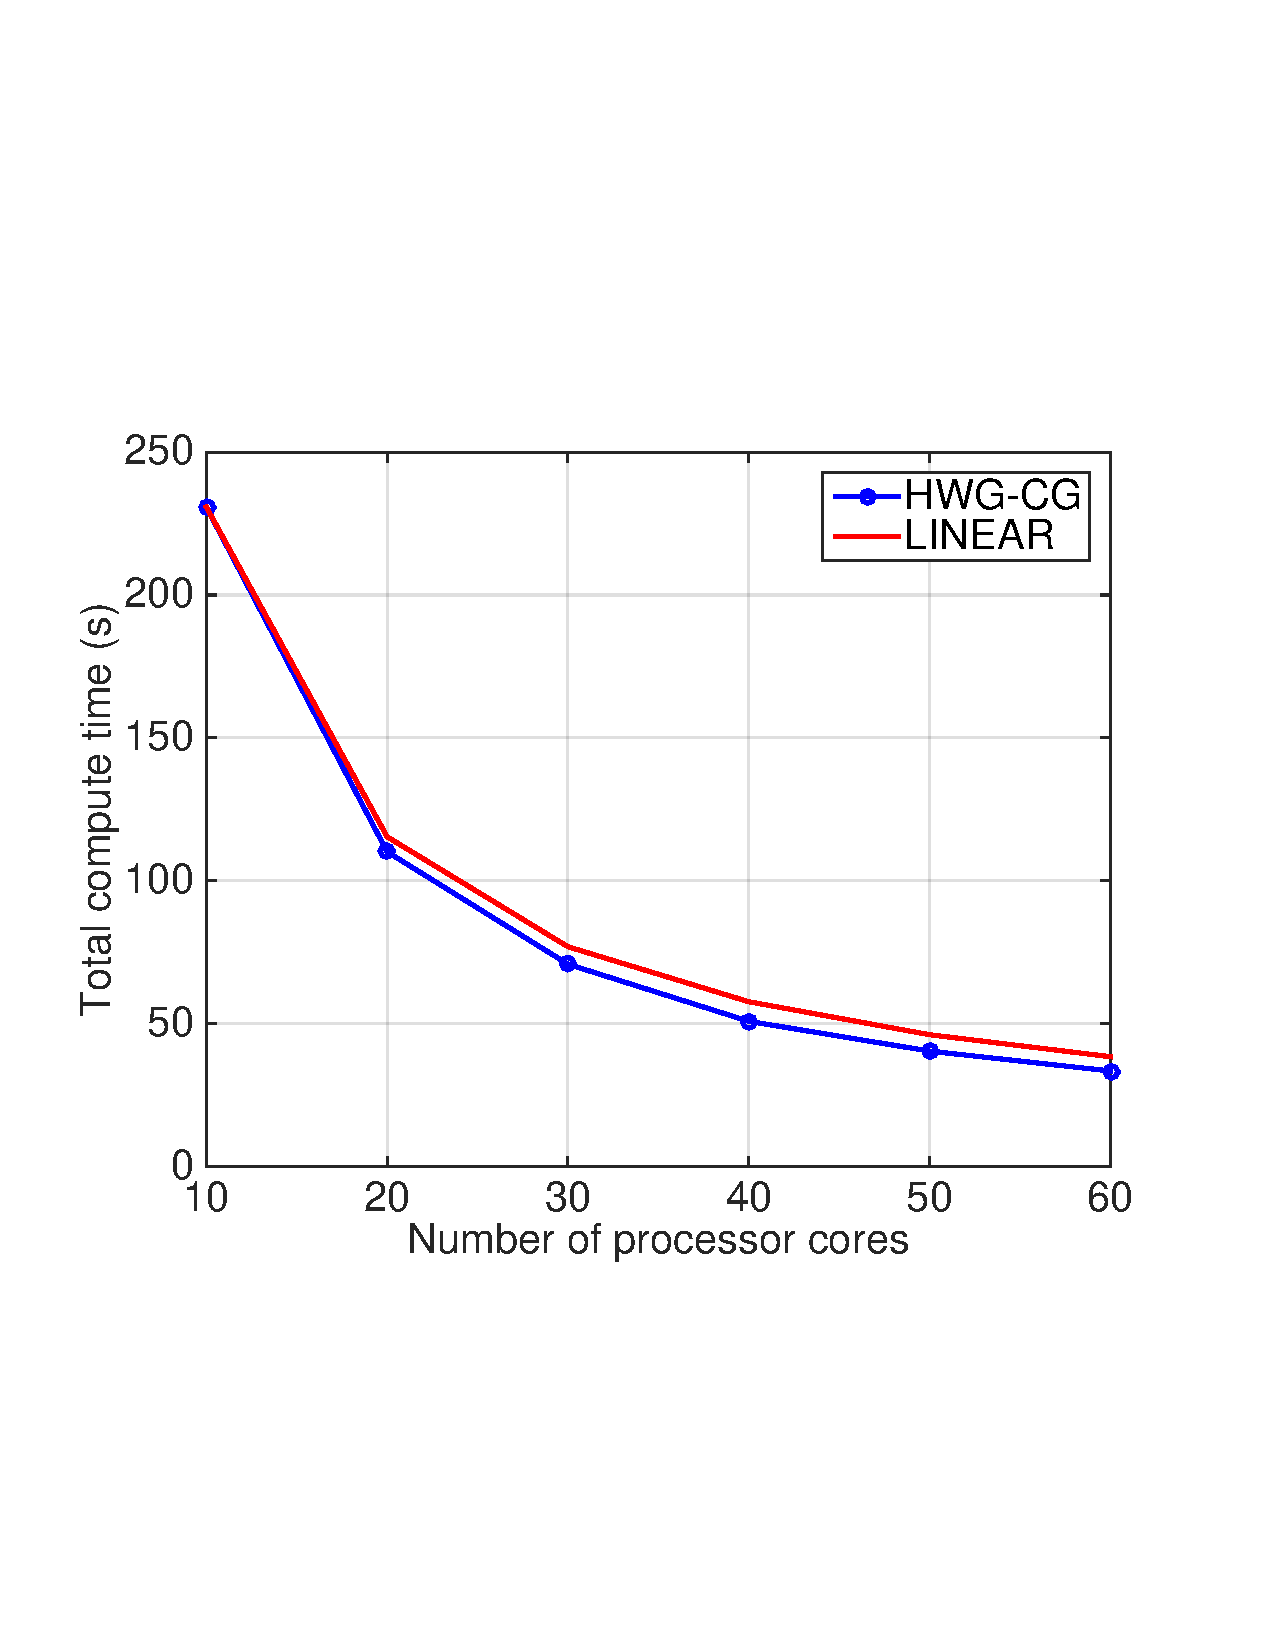
\includegraphics[width=0.7\textwidth]{./pics/lineartime}
  	\end{tabular}
  	\caption{\footnotesize Time decreasing .vs. number of processors increasing}
  \end{figure}
  
  then we also plot the speedup curvature is proportional to the increasing number of processors
   
   \begin{figure}[H]
   	\centering
   	\begin{tabular}{c}
   		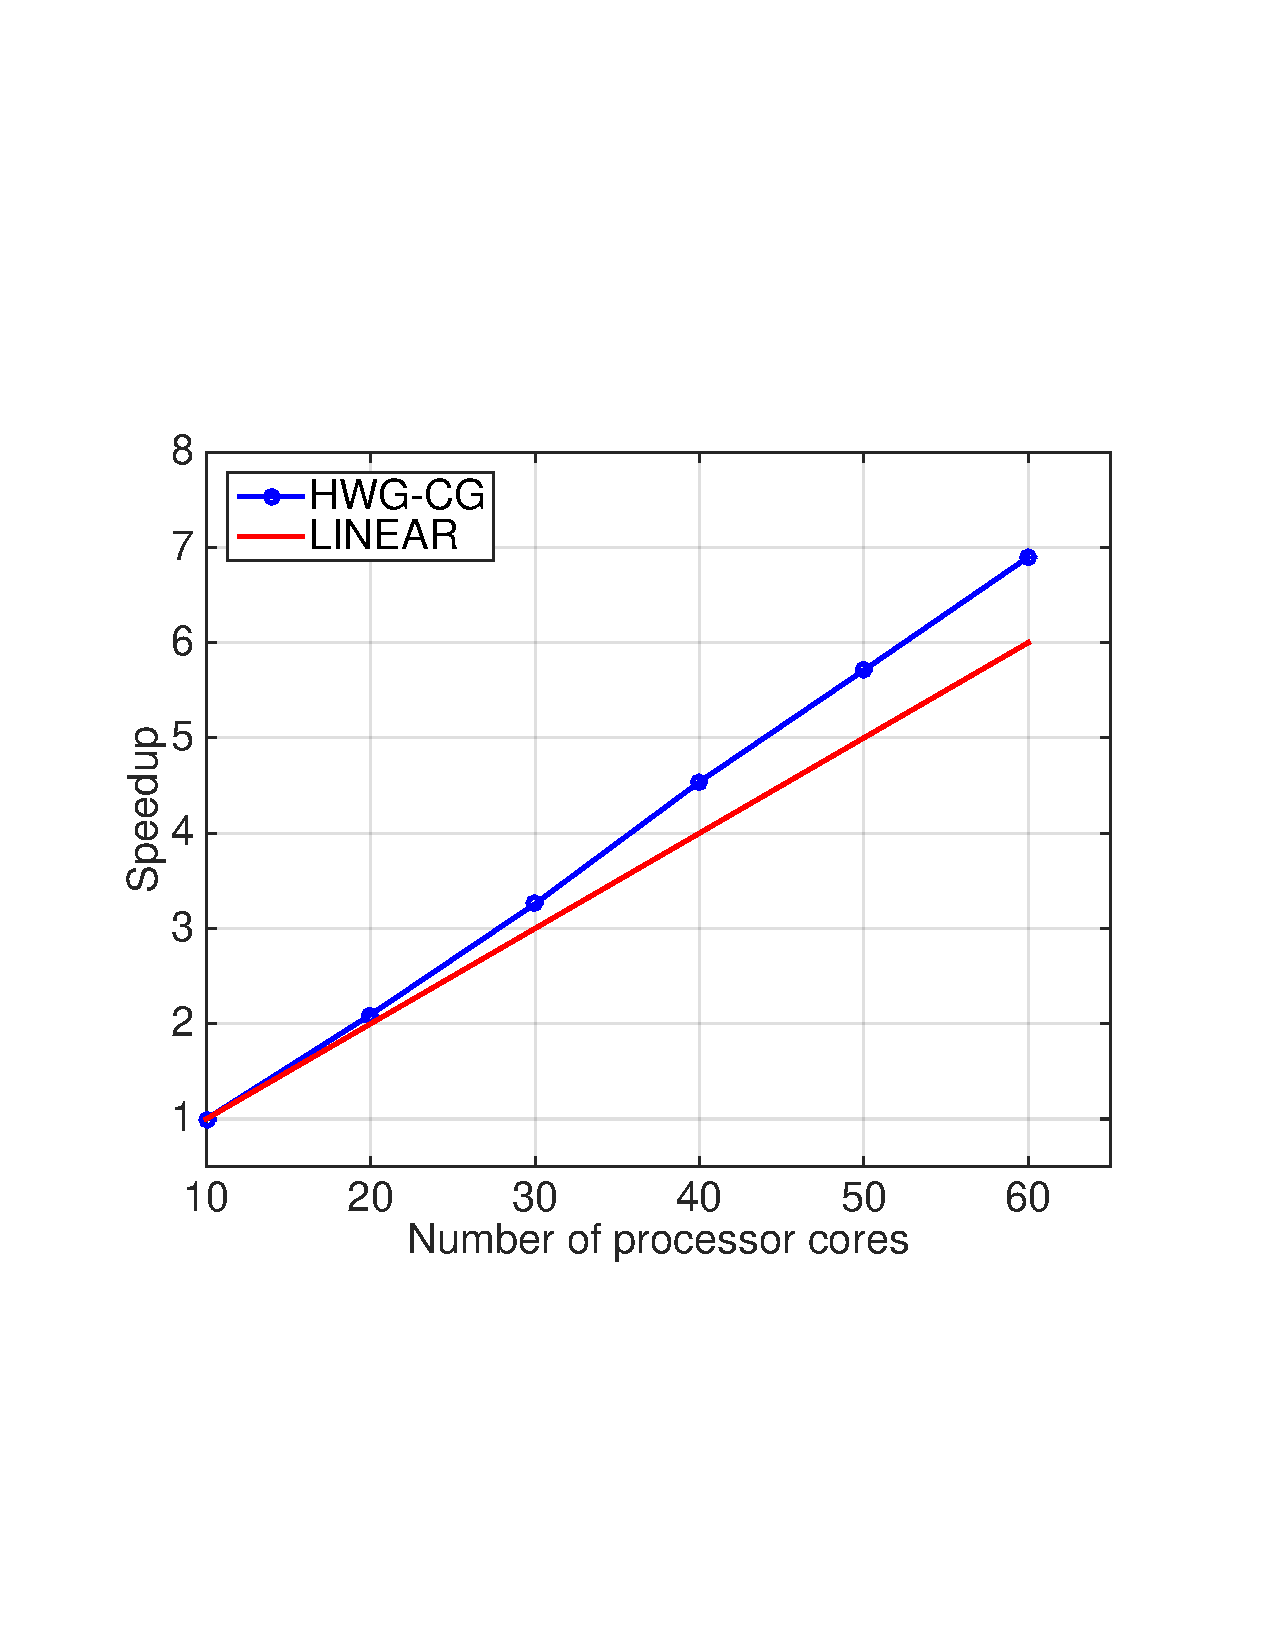
\includegraphics[width=0.7\textwidth]{./pics/linearSp}
   	\end{tabular}
   	\caption{\footnotesize Speedup .vs. number of processors increasing}
   \end{figure}
   
   A superlinear speedup is observed from the above test cases. The reason is that the computational effort to solve local matrices decreases faster than communication overhead. The computational cost for stiffness matrix inverion is $ O(n^{3}) $, where $ n $ is the size of stiffness matrix. Meanwhile, the communication overhead grows linearly with time complexity $ O(n) $.  Overall, the trade-off benefit for domain decomposition is larger than MPI communication which leads to the superlinear results. 
   
   
   		\section{Summary}
   		
   		In summary, we present a newly developed hybrid element combining the weak Galerkin finite element and continuous Galerkin finite element. It inherits the discontinuous feature from WG method and the computational simplicity from CG method. The implementation of hybrid element for parallel computing is through Schur complement method. The second order of accuracy and superlinear speedup are observed for the hybrid element. 
   		
   		We test the hybrid WG-CG element for linear and nonlinear elasticity equations. We implement explicit (Central Difference) and implicit (Newmark-Beta) methods to obtain the results. Comparing with analytical solution and published results, the error is lower than $ 10^{-5} $ for both Dirichlet and Neumann boundary condition.
   		
   		After the one dimensional examples, we present the test cases of the WG method for solving two dimensional problems.We obtain expected order of accuracy. The next step is to implement parallel computing scheme on it. The details of parallel computing for larger problem will be discussed in the next chapter.

\chapter{Weak Galerkin Parallel Solutions of Linear Elasticity on Unstructured Meshes}

This chapter focuses on solving linear elasticity problem on parallel computer by combining a novel finite element method with an efficient parallel computing scheme. Specifically, this combination involves a discontinuous weak Galerkin finite element method \cite{mu2012weak, li2013weak, wang2014weak, mu2013computational} and a non-overlapping domain decomposition scheme, namely, the balancing domain decomposition with constraints (BDDC) \cite{dohrmann2003preconditioner,tu2007three2d,tu2007three3d}. The WG method is considered as a newly developed robust numerical method and inherits the locking-free feature for the linear elastic equation \cite{wang2016locking}. 

Like the standard Finite Element method (FEM), the WG method can be used to solve generic partial differential equations. An advanced feature of the WG finite element method is that the entire problem is decomposed into multiple elemental problems. Such elemental problems are often derived from weak formulations of the corresponding differential operators after integration by parts. In these elemental problems, the differential operators are approximated and reconstructed by smaller-size matrices. The WG method has been proven robust and possessing optimal orders of accuracy in spatial discretization on serial computers \cite{mu2014weak, Mu2015new}. Wang et al \cite{wang2016locking} recently extended the WG method to solve linear elasticity problems and also successfully demonstrated its locking-free property. However, the performance of the WG method on parallel computers has not yet been examined.



\section{Domain Decomposition Scheme}
The basic idea of domain decomposition is to split the computational mesh of an entire domain into many smaller meshes for a set of non-overlapping subdomains. Each subdomain contains its own set of grid elements. For finite element methods, after domain decomposition, a remaining challenging task is to connect these subdomains' interfaces by satisfying continuity constraints to correctly represent the solution of the original set of equations over the complete domain. In this work, the BDDC method is used to serve this purpose. The original balancing domain decomposition (BDD) method \cite{mandel1993balancing} has only considered two level meshes. It used a multiplicative coarse domain to correct the local fine mesh subdomain. However, the significant difference between BDDC and BDD is that the method in this paper applies the coarse problem in an additive routine rather than multiplicative manner. In this case, a more flexible of constraints will reduce the complexity and improve the efficiency. In our BDDC method, we assemble the preconditioner matrix additively in contrast to the multiplicative coarse grid correction used in the BDD method. In the BDDC method, the flexibility of choosing constraining points leads to reduced complexity of implementation and improved efficiency of computations in comparison to the standard BDD method. The details of the choice of constraints for BDDC will be discussed in this section.

\subsection{FETI-DP Method}
Finite Element Tearing and Interconnect (FETI) , first proposed by Farhat\cite{farhat1991method, farhat1994optimal, klawonn2001feti, farhat1998two, li2006feti, klawonn2006dual}, is an iterative method for solving large finite element problems generated by linear equations. Originally, FETI is proposed to solve the discontinuity when apply domain decomposition on second order elliptic partial differential equations, particularly linear elasticity equations. FETI method partitioned the entire computational domain into two level meshes, the coarse grid and fine grid. Lagrangian multiplier is employed to conquer the discontinuity between each subdomain. For the fine mesh, since local matrix is not positive definite, the pseudo-inverse is applied to convert local matrix. 

Then FETI-DP (Dual Primal) is introduced for two-dimensional problems by Farhat and Rixen\cite{farhat2001feti}. In this new method, the unknown variables along the interface is partitioned into primal and dual spaces. The continuity of the primal unknown variables along the interface, the vertices of each subdomain, is maintained by assemblage. For the rest dual spaces, the constrains are still controlled by Lagrange multipliers. However, this constrain is only at the convergence of the method.

In this section, we begin with an example of a two-dimensional, two partitioned subdomain case. We enforce the Dirichlet boundary condition on the boundary. The original geometry and computational domain is  

\begin{figure}[h]
	\centering
	\begin{tabular}{c}
		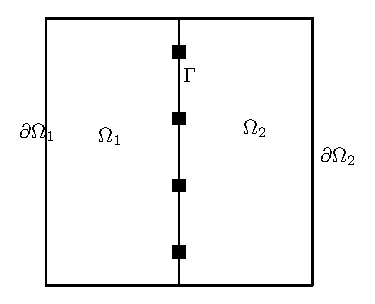
\includegraphics[width=0.6\textwidth]{./pics/feti1}
	\end{tabular}
	\caption{\footnotesize Computational domain partitioned into two nonoverlapping subdomains.}\label{fig4: feti1}
\end{figure}

the original governing equation in matrix form is $ \mathbf{A} \mathbf{u} = \mathbf{f} $. We begin to compute the stiffness matrix for each subdomain that

\begin{equation}
 \begin{pmatrix}
A_{II}^{(j)} & A_{I\Gamma}^{(j)} \\
A_{\Gamma I}^{(j)} & A_{\Gamma \Gamma}^{(j)}
\end{pmatrix} \begin{pmatrix}
u_{I}^{(j)} \\ u_{\Gamma}^{(j)}
\end{pmatrix} = \begin{pmatrix}
f_{I}^{(j)} \\ f_{\Gamma}^{(j)}
\end{pmatrix}
\end{equation}
where $ j = 1, 2 $.


The boundary condition along $ \partial \Omega  $ is Dirichlet condition, a homogeneous Neumann condition is applied on $ \Gamma $.

The global problem after assemblage is that
\begin{equation}
\begin{pmatrix}
A_{II}^{(1)} & 0 & A_{I\Gamma}^{(1)} \\
0 & A_{II}^{(2)} & A_{I\Gamma}^{(2)} \\
A_{\Gamma I}^{(1)} & A_{\Gamma I}^{(2)} & A_{\Gamma \Gamma}\\
\end{pmatrix} \begin{pmatrix}
u_{I}^{(1)} \\ u_{I}^{(2)} \\ u_{\Gamma}
\end{pmatrix} = \begin{pmatrix}
f_{I}^{(1)} \\ f_{I}^{(2)} \\ f_{\Gamma}
\end{pmatrix}
\end{equation}
where $ A_{\Gamma} = A_{\Gamma \Gamma}^{(1)} + A_{\Gamma \Gamma}^{(2)} $ and $ f_{\Gamma} = f_{\Gamma}^{(1)} + f_{\Gamma}^{(2)} $. The unknown variables are decomposed into two computational subdomains. The DOFs are represented by $ \Omega_{1}, \Omega_{2} $ and $ \Gamma $ respectively.

Since the interior matrix are square and can be inversed. Then we can eliminate the interior unknown variables by Schur complement operators. The interface unknown DOFs shall have the new form as
\begin{equation}
S^{(j)} := A_{\Gamma \Gamma}^{(j)} - A_{\Gamma I}^{(j)} {A_{II}^{(j)}}^{-1}A_{I \Gamma}^{(j)}
\end{equation}

\begin{equation}
g_{\Gamma}^{(j)} := f_{\Gamma}^{(j)} - A_{\Gamma I}^{(j)} {A_{II}^{(i)}}^{-1} f_{I}^{(j)}
\end{equation}

based on the given matrix $ Au = f $, we can reduce the equation matrices into interface DOF only system

\begin{equation}
(S^{(1)} + S^{(2)}) u_{\Gamma} = g_{\Gamma}^{(1)} + g_{\Gamma}^{2}
\end{equation}

Now we can find that the original large matrix $ A $ is reduced to a small global matrix $ S^{(j)} $ which times unknown variable vector along the interface. The interior unknown variables can be recovered locally based the solution of interface.

For FETI method, we introduce the Lagrange multiplier to enforce the continuity along the interface. The governing equation in matrix form is 
\begin{equation}
\begin{pmatrix}
A_{II}^{(j)} & A_{I \Gamma}^{(j)} \\
A_{\Gamma I}^{(j)} & A_{\Gamma \Gamma}^{(j)} \\
\end{pmatrix} \begin{pmatrix}
u_{I}^{(j)} \\ u_{\Gamma}^{(j)} 
\end{pmatrix} = \begin{pmatrix}
f_{I}^{(j)} \\ f_{\Gamma}^{(j)} + \lambda_{\Gamma}^{(j)}
\end{pmatrix}
\end{equation}
where $ j = 1, 2 $ and $ \lambda_{\Gamma} = \lambda_{\Gamma}^{(1)} = - \lambda_{\Gamma}^{(2)} $. $ \lambda_{\Gamma} $ is an unknown flux vector, namely, Lagrange multiplier. We can solve this linear system following previous fashion that

\begin{equation}
g_{\Gamma}^{(j)} = f_{\Gamma}^{(j)} - A_{\Gamma I}^{(j)} {A_{II}^{(j)}}^{-1} f_{I}^{(j)}
\end{equation}

\begin{equation}
u_{\Gamma}^{(j)} = {S^{(j)}}^{-1} (g_{\Gamma}^{(j)} + \lambda_{\Gamma}^{(j)})
\end{equation}

to maintain the continuity along the interface, the condition is set as
\begin{equation}
u_{\Gamma}^{(1)} = u_{\Gamma}^{(2)}
\end{equation}
the value of DOFs for the same position has to be same. To resolve the rigid body motion problem, we obtain
\begin{equation}
F \lambda_{\Gamma} = d_{\Gamma}
\end{equation}
\begin{equation}
F = {S^{(1)}}^{-1} + {S^{(2)}}^{-1}
\end{equation}

An improved version of FETI is FETI-DP. We can partitioned the subdomains with floating constraints.

\begin{figure}[h]
	\centering
	\begin{tabular}{c}
		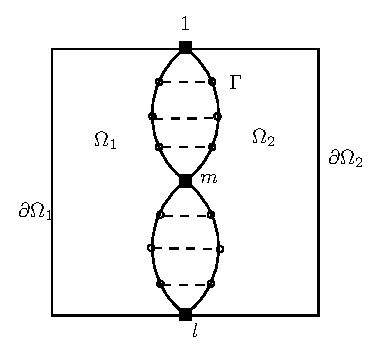
\includegraphics[width=0.5\textwidth]{./pics/feti2}
	\end{tabular}
	\caption{\footnotesize Computational domain partitioned into two nonoverlapping subdomains with floating constaint.}
\end{figure}

From the above figure, the interface edge is continued to split into $ (u_1, \cdots, u_m, \cdots, u+l) $ then the linear system can be written as

\begin{equation}
\begin{pmatrix}
A_{II}^{(j)} & A_{1I}^{(j)} & \cdots & A_{mI}^{(j)} & \cdots & A_{l I}^{(j)} \\
A_{1 I}^{(j)} & A_{11}^{(j)} & \cdots & A_{1m}^{(j)} & \cdots & A_{1l}^{(j)} \\
\vdots & \vdots & \ddots & \vdots & \ddots & \vdots \\
A_{mI}^{(j)} & A_{m1}^{(j)} & \cdots & A_{mm}^{(j)} & \cdots & A_{ml}^{(j)} \\
\vdots & \vdots & \ddots & \vdots & \ddots & \vdots \\
A_{lI}^{(j)} & A_{l1}^{(j)} & \cdots & A_{lm}^{(j)} & \cdots & A_{ll}^{(j)}\\
\end{pmatrix} \begin{pmatrix}
u_{I}^{(j)} \\ u_{1}^{(j)} \\ \vdots \\ u_{m}^{(j)} \\ \vdots \\ u_{l}^{(j)}\\
\end{pmatrix} = \begin{pmatrix}
f_{I}^{(j)} \\ f_{1}^{(j)} \\ \vdots \\ f_{m}^{(j)} \\ \vdots \\ f_{l}^{(j)}
\end{pmatrix}
\end{equation}

The variable along the interface of two nonoverlapping subdomian can be elaborate as
\begin{equation}
\begin{pmatrix}
u_{1}^{(j)} \\ \vdots \\ u_{m}^{(j)} \\ \vdots \\ u_{l}^{(j)}
\end{pmatrix} = T_{E} \begin{pmatrix}
\hat{u}_{1}^{(j)} \\ \vdots \\ \hat{u}_{m}^{(j)} \\ \vdots \\ \hat{u}_{l}^{(j)}
\end{pmatrix} = \begin{pmatrix}
1 & \cdots & 1 & 0 & \cdots \\
\vdots & \ddots & \vdots & 0 & \cdots \\
-1 & \cdots & 1 & \cdots & -1 \\
\cdots & 0 & \vdots & \ddots &  \vdots \\
\cdots & 0 & 1 & \cdots & 1\\
\end{pmatrix} \begin{pmatrix}
\hat{u}_{1}^{(j)} \\ \vdots \\ \hat{u}_{m}^{(j)} \\ \vdots \\ \hat{u}_{l}^{(j)}
\end{pmatrix}
\end{equation}

After the multiplication between vector and matrix we have
\begin{equation}
T_{E} \begin{pmatrix}
\hat{u}_{1}^{(j)} \\ \vdots \\ \hat{u}_{m}^{(j)} \\ \vdots \\ \hat{u}_{l}^{(j)}
\end{pmatrix} = \begin{pmatrix}
1 \\ \vdots \\ 1 \\ \vdots \\ 1
\end{pmatrix} \hat{u}_{m}^{(j)} + \begin{pmatrix}
& & \hat{u}_{1}^{(j)} & & \\
& & \vdots & & \\
-\hat{u}_{1}^{(j)} & -\cdots & -\hat{u}_{m-1}^{(j)} & \hat{u}_{m+1}^{(j)} & -\hat{u}_{l}^{(j)}\\
& & \vdots & & \\
& & \hat{u}_{l}^{(j)} & & \\
\end{pmatrix}
\end{equation}
the $ T_{E} $ is a square matrix and the columns representing the new space of interface unknown variables. The original interface is divided into two parts. One part is that the value of unknown variables has a value on its own subdomain. The other part is that the function has zero interface averages. The the problem can be rewrite as

\begin{equation}
T^{T} \begin{pmatrix}
A_{II}^{(j)} & A_{1I}^{(j)} & \cdots & A_{mI}^{(j)} & \cdots & A_{l I}^{(j)} \\
A_{1 I}^{(j)} & A_{11}^{(j)} & \cdots & A_{1m}^{(j)} & \cdots & A_{1l}^{(j)} \\
\vdots & \vdots & \ddots & \vdots & \ddots & \vdots \\
A_{mI}^{(j)} & A_{m1}^{(j)} & \cdots & A_{mm}^{(j)} & \cdots & A_{ml}^{(j)} \\
\vdots & \vdots & \ddots & \vdots & \ddots & \vdots \\
A_{lI}^{(j)} & A_{l1}^{(j)} & \cdots & A_{lm}^{(j)} & \cdots & A_{ll}^{(j)}\\
\end{pmatrix} T \begin{pmatrix}
u_{I}^{(j)} \\ \hat{u}_{1}^{(j)} \\ \vdots \\ \hat{u}_{m}^{(j)} \\ \vdots \\ \hat{u}_{l}^{(j)}\\
\end{pmatrix} = T^{T} \begin{pmatrix}
f_{I}^{(j)} \\ f_{1}^{(j)} \\ \vdots \\ f_{m}^{(j)} \\ \vdots \\ f_{l}^{(j)}
\end{pmatrix}
\end{equation}

same as previous equation, $ T $ is a diagonal block matrix 
\begin{equation}
T = \begin{pmatrix}
I & 0 \\ 
0 & T_{E}\\
\end{pmatrix}
\end{equation}

We find out that the change is an individual interface edge local procedure. We can assume that the unknown variables on each subdomain have been changed when using primal edges or faces. In last figure, we can see that the primal space is the only connection along the interface. The other DOFs are in dual space including interior unknowns and the rest interface nodes.

\begin{equation}
\begin{pmatrix}
A_{II}^{(1)} &  A_{\Delta I}^{(1)}& 0 & 0 & A_{\Pi I}^{(1)} & 0 \\
A_{\Delta I}^{(1)} & A_{\Delta \Delta}^{(1)} & 0 & 0& A_{\Pi \Delta}^{(1)} & B_{\Delta}^{(1)}\\
0 & 0 & A_{II}^{(2)} & A_{\Delta I}^{(2)} & A_{\Pi I}^{(2)} & 0 \\
0 & 0 & A_{\Delta I}^{(2)} & A_{\Delta \Delta}^{(2)} & A_{\Pi \Delta}^{(2)} & B_{\Delta}^{(2)} \\
A_{\Pi I}^{(1)} & A_{\Pi \Delta}^{(1)} & A_{\Pi I}^{(2)} & A_{\Pi \Delta}^{(2)} & A_{\Pi \Pi}^{(1)} + A_{\Pi \Pi}^{(2)} & 0 \\
0 & B_{\Delta}^{(1)} & 0 & B_{\Delta}^{(2)} & 0 & 0 \\
\end{pmatrix} \begin{pmatrix}
u_{I}^{(1)} \\ u_{\Delta}^{(1)} \\ u_{I}^{(2)} \\ u_{\Delta}^{(2)} \\ u_{\Pi} \\ \lambda\\
\end{pmatrix} = \begin{pmatrix}
f_{I}^{(1)} \\ f_{\Delta}^{(1)} \\ f_{I}^{(2)} \\ f_{\Delta}^{(2)} \\ f_{\Pi}^{(1)} + f_{\Pi}^{(2)} \\ 0\\
\end{pmatrix}
\end{equation}

We can further eliminate the local variables $ u_{I}^{(1)}, u_{\Delta}^{(1)}, u_{I}^{(2)} $ and $ u_{\Delta}^{(2)} $, so that we can obtain
\begin{equation}
\begin{pmatrix}
S_{\Pi \Pi} & \tilde{B}_{\Lambda \Pi}^{T} \\ 
\tilde{B}_{\Lambda \Pi} & \tilde{B}_{\Lambda \Lambda} \\
\end{pmatrix} \begin{pmatrix}
u_{\Pi} \\ \lambda \\
\end{pmatrix} = \begin{pmatrix}
g_{\Pi} \\ d_{\Lambda}\\
\end{pmatrix}
\end{equation}

the details of above equation is 

\begin{equation}
S_{\Pi \Pi} = \sum_{j = 1}^{2} R_{\Pi}^{(j)} \begin{pmatrix}
A_{\Pi \Pi}^{(j)} - \begin{bmatrix}
A_{\Pi I}^{(j)} & A_{\Pi \Delta}^{(j)} \\
\end{bmatrix} \begin{bmatrix}
A_{II}^{(j)} & A_{I \Delta}^{(j)} \\
A_{\Delta I}^{(j)} & A_{\Delta \Delta}^{(j)}
\end{bmatrix}^{-1} \begin{bmatrix}
A_{\Pi I}^{(j)} \\ A_{\Pi \Delta}^{(j)} \\
\end{bmatrix}
\end{pmatrix} R_{\Pi}^{(j)} ,
\end{equation}

\begin{equation}
\tilde{B}_{\Lambda \Pi} = - \sum_{j = 1}^{2} \begin{bmatrix}
0 & B_{\Pi}^{(j)}
\end{bmatrix} \begin{bmatrix}
A_{II}^{(j)} & A_{\Delta I}^{(j)} \\
A_{\Delta I}^{(j)} & A_{\Delta \Delta}^{(j)}
\end{bmatrix}^{-1} \begin{bmatrix}
A_{\Pi I}^{(j)} \\ A_{\Pi \Delta}^{(j)}
\end{bmatrix} R_{\Pi}^{(j)} ,
\end{equation}

\begin{equation}
\tilde{B}_{\Lambda \Lambda} = - \sum_{j = 1}^{2} \begin{bmatrix}
0 & B_{\Delta}^{(j)}
\end{bmatrix} \begin{bmatrix}
A_{II}^{(j)} & A_{\Delta I}^{(j)} \\
A_{\Delta I}^{(j)} & A_{\Delta \Delta}^{(j)}
\end{bmatrix}^{-1} \begin{bmatrix}
0 \\B_{\Delta}^{(j)} \\
\end{bmatrix} ,
\end{equation}

\begin{equation}
g_{\Pi} = \sum_{j = 1}^{2} R_{\Pi}^{(j)} \begin{pmatrix}
f_{\Pi}^{(j)} - \begin{bmatrix}
A_{\Pi I}^{(j)} & A_{\Pi \Delta}^{(j)}
\end{bmatrix} \begin{bmatrix}
A_{II}^{(j)} & A_{\Pi \Delta}^{(j)} \\
\end{bmatrix} \begin{bmatrix}
A_{II}^{(j)} & A_{\Delta I}^{(j)} \\
A_{\Delta I}^{(j)} & A_{\Delta \Delta}^{(j)}\\
\end{bmatrix}^{-1} \begin{bmatrix}
f_{I}^{(j)} \\ f_{\Delta}^{(j)}
\end{bmatrix}
\end{pmatrix} ,
\end{equation}

\begin{equation}
d_{\Lambda} = - \sum_{j = 1}^{2} \begin{bmatrix}
0 & B_{\Delta}^{(j)} \\
\end{bmatrix} \begin{bmatrix}
A_{II}^{(j)} & A_{\Delta I}^{(j)} \\
A_{\Delta I}^{(j)} & A_{\Delta \Delta}^{(j)} 
\end{bmatrix}^{-1} \begin{bmatrix}
f_{I}^{(j)} \\ f_{\Delta}^{(j)} \\
\end{bmatrix}
\end{equation}

whre the $ R_{\Pi}^{(j)} $ is a projection matrix that mapping the local subdomain element to global elements with $ \{0, 1\} $ values. In this example, both projection values are equal to $ 1 $.

For the linear system, the Lagrange multiplier $ \lambda $ is
\begin{equation}
\begin{pmatrix}
\tilde{B}_{\Lambda \Lambda} - \tilde{B}_{\Lambda \Pi} S_{\Pi \Pi}^{-1} \tilde{B}_{\Lambda \Pi}^{T}
\end{pmatrix} \lambda = d_{\Lambda} - \tilde{B}_{\Lambda \Pi} S_{\Pi \Pi}^{-1} g_{\Pi}
\end{equation}

A Dirichlet preconditioner is applied in FETI-DP method for solving above equation. 

Based on above linear system, we can find out that the Lagrange multiplier is an external unknown vector and requires lots of computational effort to assemble the matrix. When we solve the such a linear system, it's common to obtain the result along the dual space that $ u_{\Delta}^{(1)} \neq  u_{\Delta}^{(2)}$. To maintain the continuity, we shall restore the computing a weighted average of the vectors. Therefore, an assembled residual of resulting vector needs to be compute. The residue is mapped into the appropriate space of enforced vector on the right-hand side of the equation. Then we can use the residue vector to correct the solution and gradually obtain the final results. An improved algorithm, BDDC method, will be discussed in the following section.


\subsection{Balancing Domain Decomposition by Constraints}

The balancing domain decomposition method was introduced by Mandel \cite{mandel2005algebraic}. The original idea of BDD method is applying a coarse correction to guarantee the convergence of residuals. The BDDC is a domain decomposition method for solving large symmetric, positive definite equations of linear systems. The main function is to solve problems arises from the finite element method, including WG method. It is inspired by FETI-DP method of Farhat et al \cite{farhat1994optimal, farhat2001feti} which has been extended multi-dimension varying problems. Comparing to BDD method, the substructure spaces and the coarse spaces are connected by the corner cell as constraints only. The main difference is that the BDDC method applies the coarse problem in an additive routine, which makes it possible to use a different bilinear form on the coarse problem. In this way, the BDDC method is considered as a simpler primal alternative to FETI-DP domain decomposition method \cite{li2006feti}. In this paper, we only consider the corner connections of subdomain as the only constraints. The substructure spaces, coarse space, and the substructure bilinear forms are same as Mandel’s paper. Comparing with FETI-DP, BDDC method adds coarse degrees of freedom involving averages over edges and faces of elements. This improvement causes an obvious simplification through domain decomposition and matrix calculation.

After the Schur complement, the preconditioner for interface is 
\begin{equation}
\hat{S}u_{\Gamma} = \sum_{j = 1}^{N} R_{\Gamma}^{(j)} g_{\Gamma}
\end{equation}

where
\begin{equation}
\tilde{S} = \tilde{R}_{\Gamma}^{T} \tilde{S}_{\Gamma} \tilde{R}_{\Gamma}
\end{equation}

In the BDDC algorithm, a two-level Neumann-Neumann type preconditioner for solving this interface problem is as above equation. In the BDDC preconditioner, the coarse grid is assembled from coarse basis functions. We can apply the minimum energy method on the subdomains to obtain primal constrains. The primal constraints maintain the continuity along the edge interface between two subdomains, as in FETI-DP algorithm. 

Dohrmann's BDDC preconditioner \cite{dohrmann2003preconditioner, dohrmann2003study, mandel2005algebraic} has the form
\begin{equation}
M_{BDDC}^{-1} = R_{D, \Gamma}^{T} T R_{D, \Gamma}
\end{equation}
for the coarse-level $ T $ is defined by 
\begin{equation}
T = \Psi (\Psi^{T} S \Psi)^{-1} \Psi^{T}
\end{equation}
the coarse level basis function vector is defined by 
\begin{equation}
\Psi = \begin{pmatrix}
\Psi^{(1)} \\ \vdots \\ \Psi^{(N)}\\
\end{pmatrix}
\end{equation}

Then the Schur complement coarse-level matrix can be written as 
\begin{equation}
\begin{pmatrix}
S^{(j)} & {C^{(j)}}^{T} \\
C^{(j)} & 0 \\
\end{pmatrix} \begin{pmatrix}
\Psi^{(j)} \\ V^{(j)} \\
\end{pmatrix} = \begin{pmatrix}
0 \\ R_{\Pi}^{(j)}\\
\end{pmatrix}
\end{equation}
 where $ C^{(j)} $ is the primal constraints of each subdomain and $ V^{(j)} $ is Lagrange multiplier vector. If we assume the variable is changing, then the Lagrange multiplier vector is no longer needed to enforce the primal continuity constraints and the new BDDC preconditioner can be designed as
 
 \begin{equation}
 M_{BDDC}^{-1} = R_{D, \Gamma}^{T} \{ R_{\Gamma \Delta}^{T} S^{-1}_{\Delta} R_{\Gamma \Delta} + \Psi (\Psi^{T} S \Psi)^{-1} \Psi^{T} \} R_{D, \Gamma}
 \end{equation}
 
 The primal space DOFs are used to enforce the continuity by restricting the operators to the dual interface space $ \Delta $. The governing matrix equation can be designed as
 \begin{equation}
 \begin{pmatrix}
 A_{II}^{(j)} & A_{\Delta I}^{(j)} & A^{(j)}_{\Pi I} \\
 A_{\Delta I}^{(j)} & A_{\Delta \Delta}^{(j)} & A_{\Pi \Delta}^{(j)} \\
 A_{\Pi I}^{(j)} & A_{\Pi \Delta}^{(j)} & A_{\Pi \Pi}^{(j)} \\
 \end{pmatrix} \begin{pmatrix}
 u_{I}^{(j)} \\ \Psi_{\Delta}^{(j)} \\ R_{\Pi}^{(j)} \\
 \end{pmatrix} = \begin{pmatrix}
 0 \\ 0 \\ S_{\Pi \Pi}^{(j)} R_{\Pi}^{(j)}
 \end{pmatrix}
 \end{equation}

\section{WG-BDDC Method}
In this section, we discuss the details of design the parallel computing scheme by combining WG method with BDDC method. 

The preconditioned conjugate gradient method is adopted as the linear solver for BDDC method. The construction of preconditioner is crucial in the problem. The BDDC preconditioner combines the solution of the local problem on each subdomain with the solution of a global coarse problem and the coarse degrees of freedoms as unknowns. 

The preconditioned conjugate gradient method is adopted as the linear solver for BDDC method. The construction of preconditioner is crucial in the problem. The BDDC preconditioner combines the solution of the local problem on each subdomain with the solution of a global coarse problem and the coarse degrees of freedoms as unknowns. 

In FETI method, local matrices after domain decomposition are singular and the pseudo-inverses must be computed. On the contrary, the WG-BDDC has the advantage to bypass this difficulty.

BDDC shall be processed by the following steps:

\begin{figure}[h]
	\centering
	\begin{tabular}{c}
		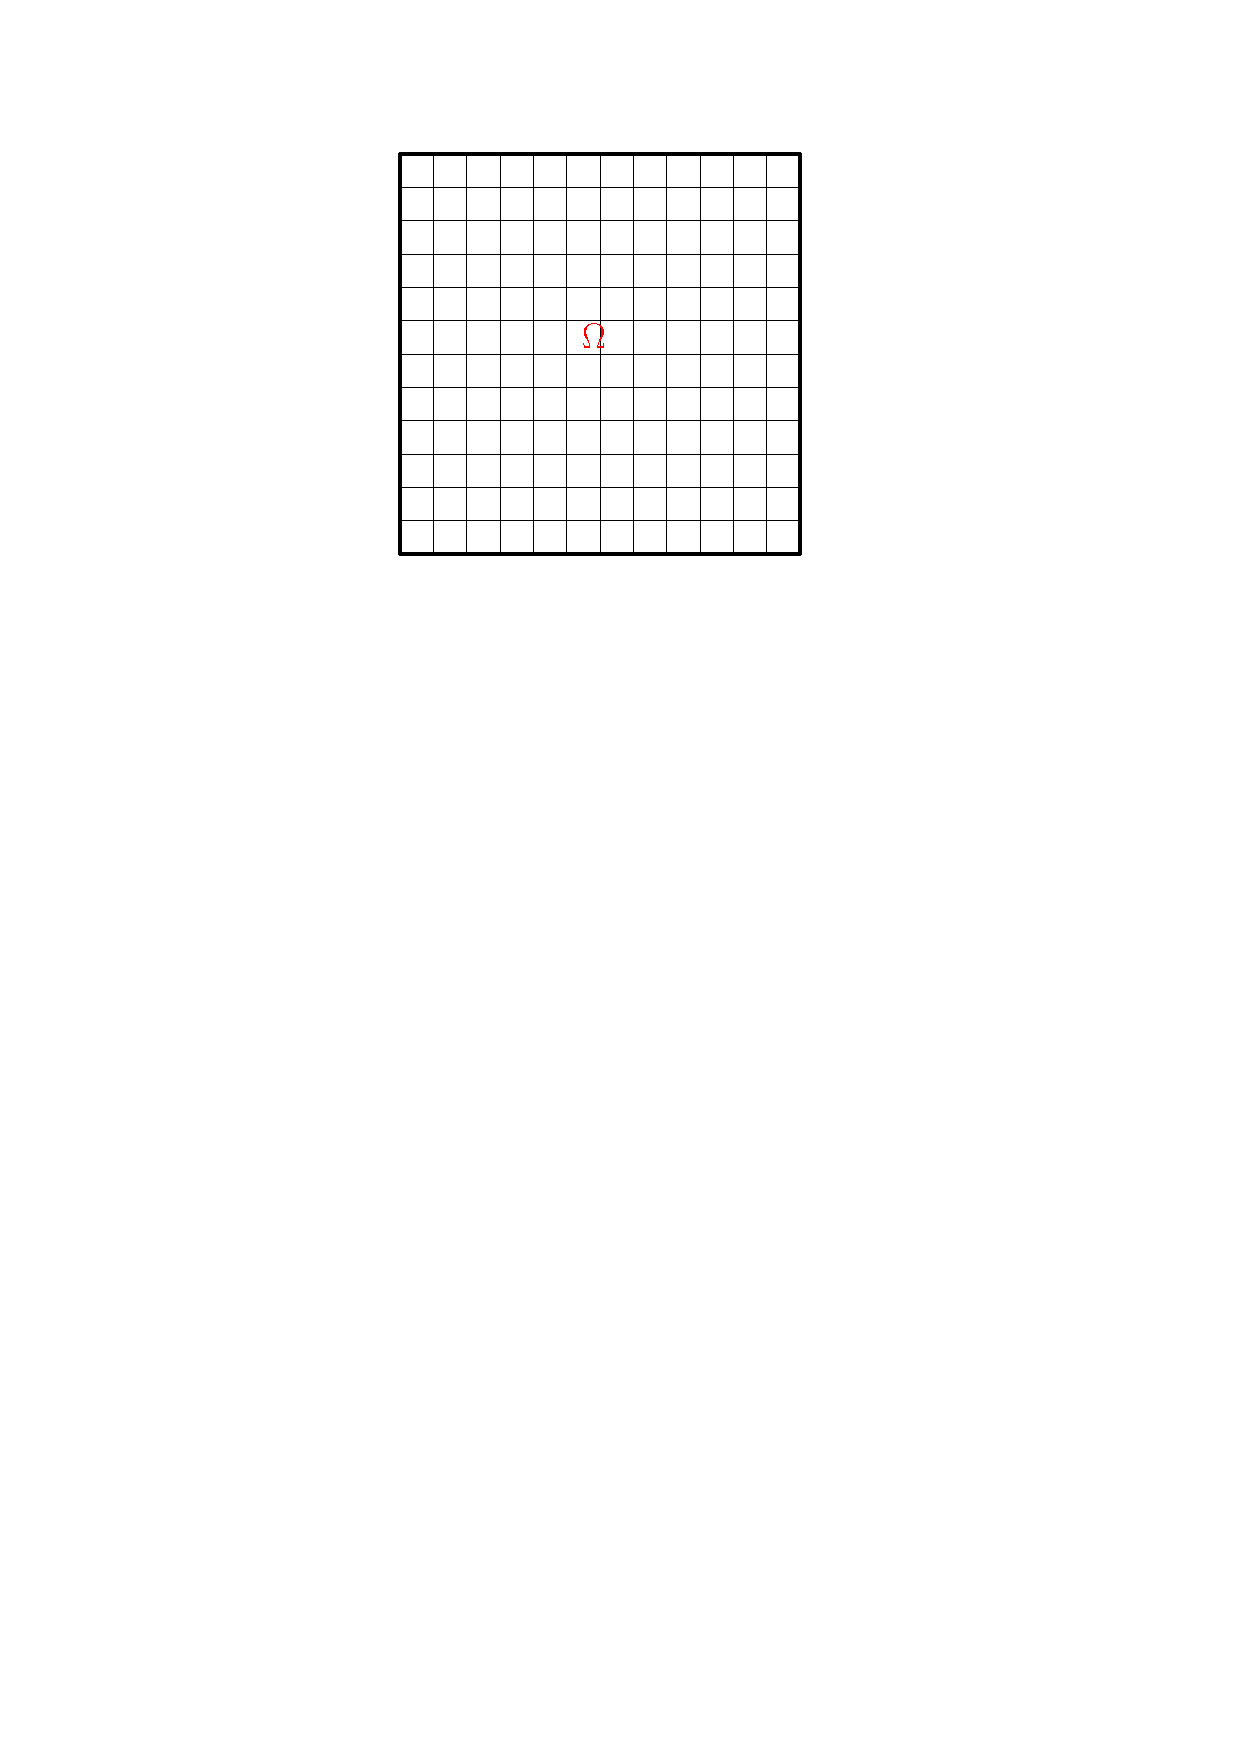
\includegraphics[width=0.5\textwidth]{./pics/domain.pdf}
	\end{tabular}
	\caption{\footnotesize The total computational domain.}\label{fig3: domain}
\end{figure}

\begin{enumerate}
	\item	Schur Complement \cite{duff1986direct} of problems on each subdomain  will eliminate all the interior unknowns and only retain the unknowns on the interface of . Denote the interface by .
	\item	Reduce the unknowns on the interface to construct the preconditioner.
	\item	Solve the linear system by using preconditioned conjugate gradient solver.
\end{enumerate}


\begin{figure}[h]
	\centering
	\begin{tabular}{c}
		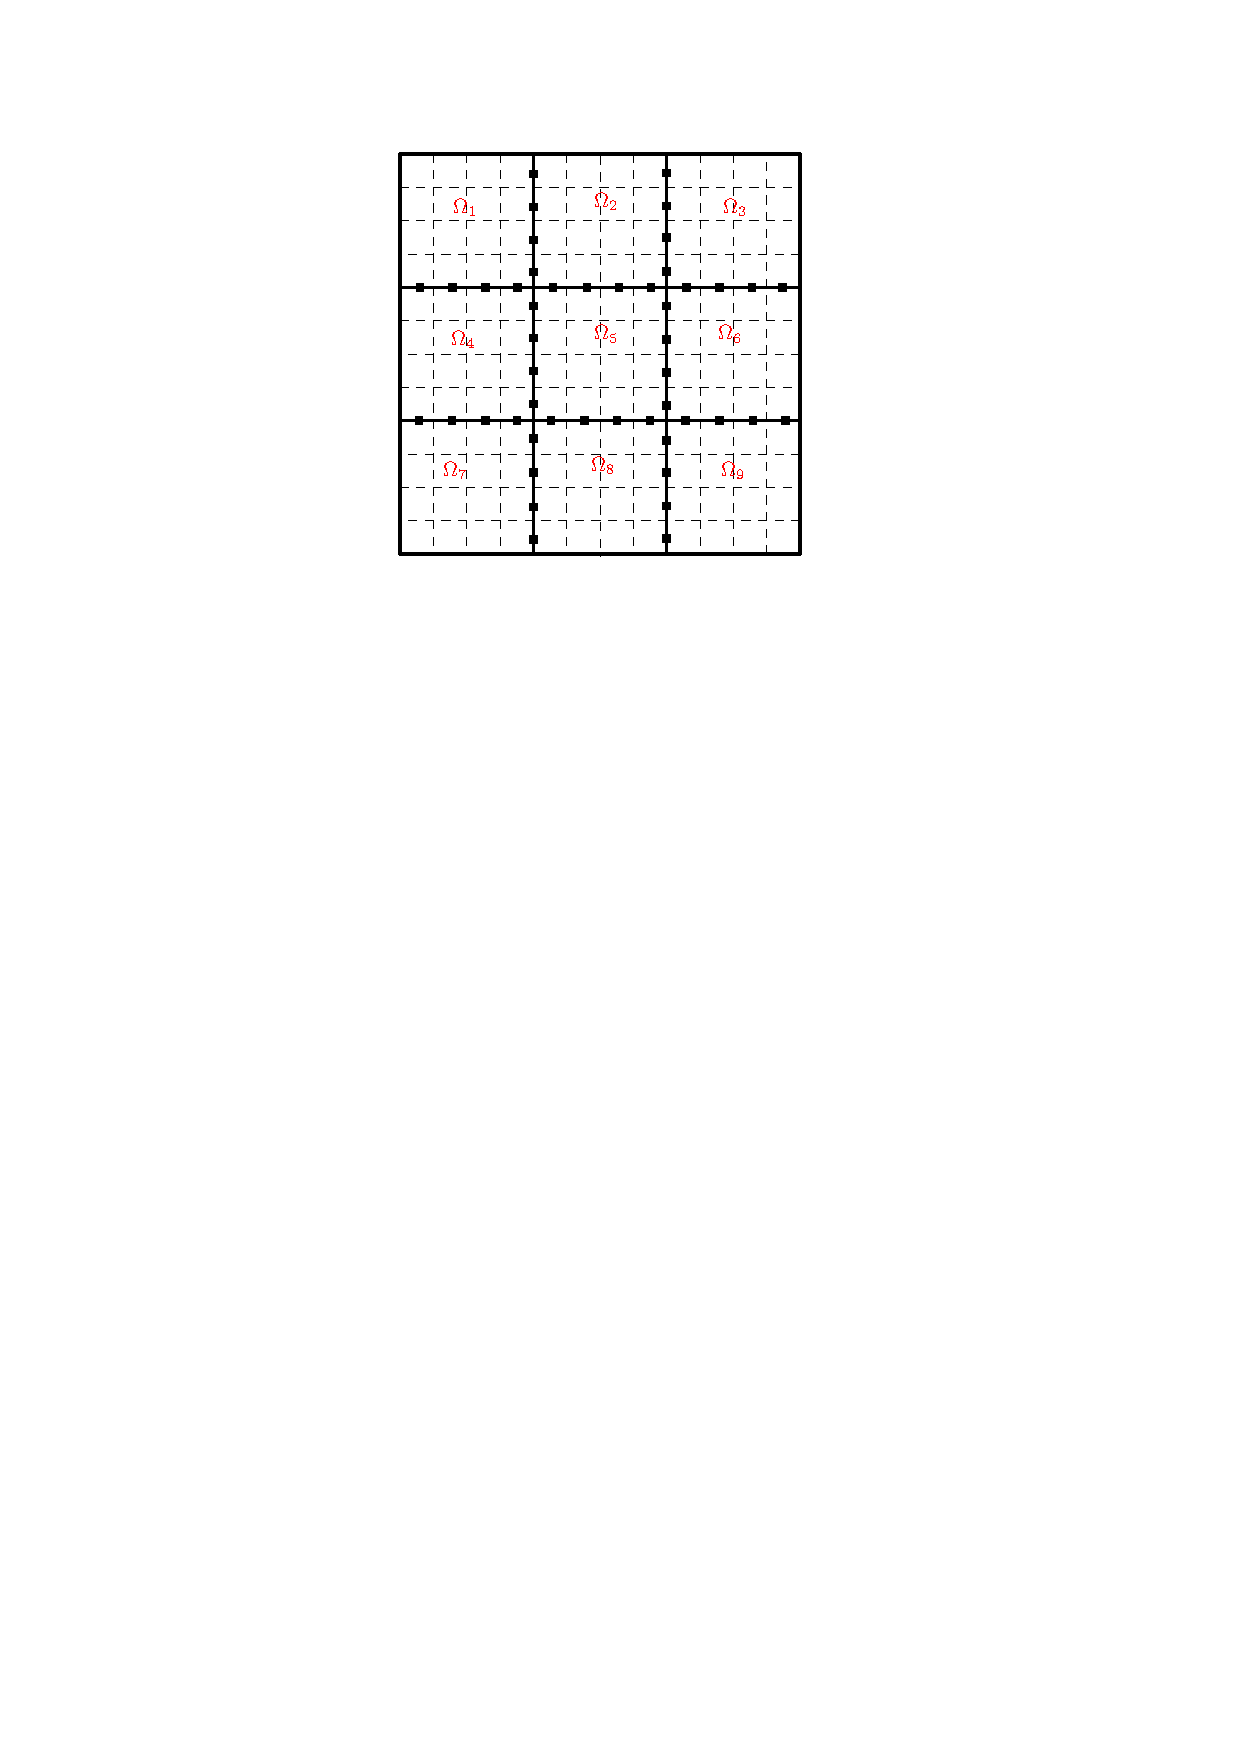
\includegraphics[width=0.6\textwidth]{./pics/domain2.pdf}
	\end{tabular}
	\caption{\footnotesize After the Schur complement method the computational domain becomes interior and interface.}\label{fig4: domain1}
\end{figure}

In the second step, the solid dot represents the unknown variables along the interface. They are shared by adjacent subdomains and should be calculated in the global matrix through Schur complement method. Even though the number of DOF in global matrix is drastically decreased, the communication overhead and scale of global matrix are still not satisfied the standard for high performance computing. In this way, we shall continuously split the interface into two spaces.


\begin{figure}[h]
	\centering
	\begin{tabular}{c}
		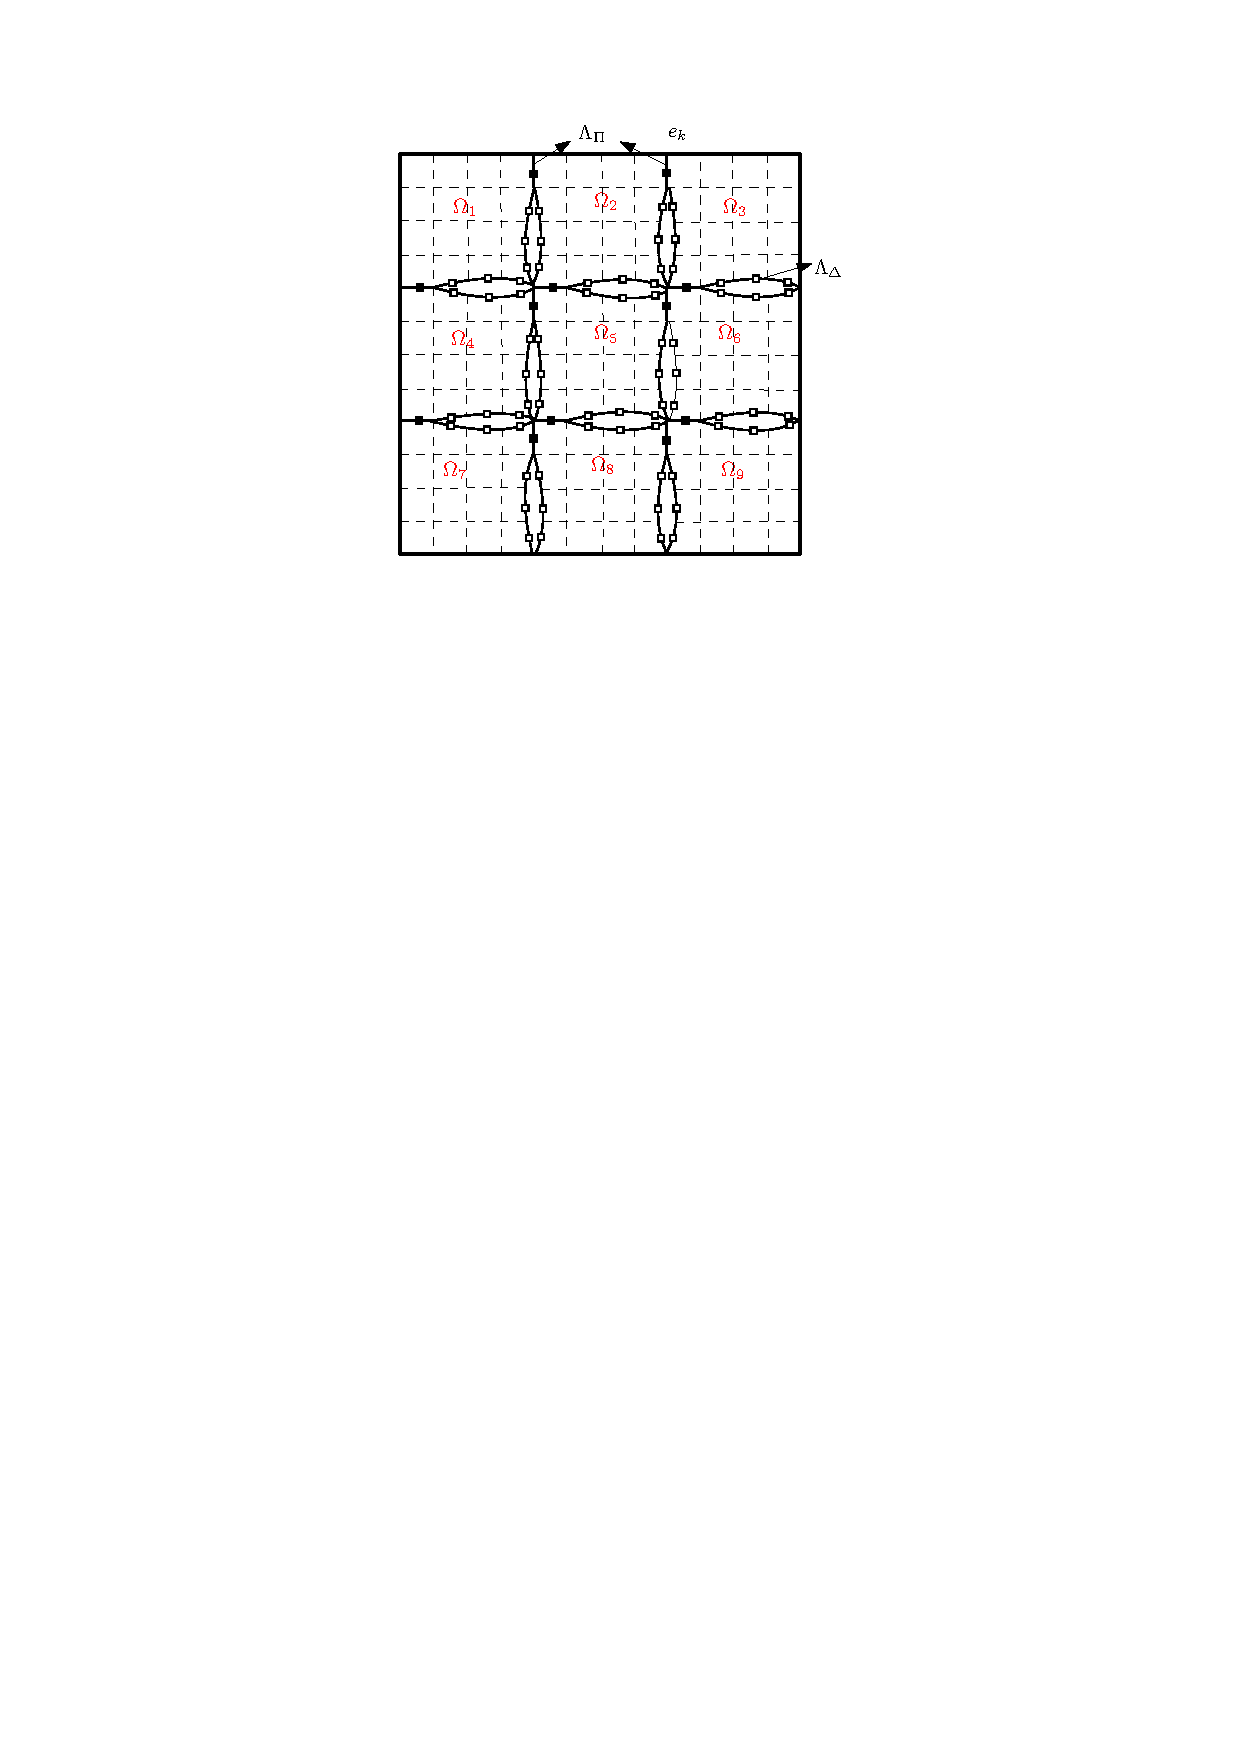
\includegraphics[width=0.6\textwidth]{./pics/domain3.pdf}
	\end{tabular}
	\caption{\footnotesize BDDC computational domain with only one cell boundary.}\label{fig5: domain2}
\end{figure}

In the third graph, we split the interface into primal and dual spaces. The circle represents the unknown variables belongs to dual space. They are calculated only in local matrices. We bridged the information from dual space to primal space through preconditioner. The remain dots are unknown variables in the primal spaces. They are the only information shall be communicated and calculated through MPI functions. Now the global matrix has been decreased to an optimal level which benefit us significantly in speedup test. 

One significant feature of this method is that when the number of subdomains increasing, the condition number of this method is bounded under the circumstance that an appropriate choice of the coarse DOFs and with regular subdomain shapes. The condition number grows only very slowly with the number of elements in each subdomain.

The number of iterations is also bounded in the same fashion. Meanwhile, the method scales well with the number of subdomains and size of the problem. 

\section{Schur Complement Method for subdomain $ \Omega_{j} $}

Denote the weak Galerkin solution on each subdomain $ \Omega_{j} $  For the consistency with Equation (1), we will use $ u_{h} $  to represent the weak Galerkin solution on each $ \Omega_{j} $.

To define the Schur complement system, the degrees of freedom $ u_h $  on each subdomain $ \Omega_j $ are partitioned into interior  $ u_{I}  $and interface $ u_{\Gamma} $ parts . Then, we can rewrite the unknown variable function as 
\begin{equation}
u_{h} = [u_{I0}, u_{Ib}, u_{\Gamma b}]
\end{equation}
and denote  $ u_I =  [u_{I0}, u_{Ib}]$, meanwhile, the $ u_{\Gamma} = u_{\Gamma b} $ . Consequently, the local Schur complements can be applied to each subdomain  in the following form
\begin{equation}
\begin{pmatrix}
A_{II} & A_{\Gamma I}^{T} \\
A_{\Gamma I} & A_{\Gamma \Gamma} \\
\end{pmatrix} \times
\begin{pmatrix}
u_{I} \\ u_{\Gamma}
\end{pmatrix}
\end{equation}

To define the Schur complement system, the DOFs on each subdomain are partitioned by interior and interface categories. Now the unknown function becomes $ u_{h} = [u_{I0}, u_{Ib}, u_{\Gamma b}] $, $ v_{h} = [v_{I0}, v_{Ib}, v_{\Gamma b}] $ and denote the interior unknown variable $ u_{i} = [u_{I0}, u_{Ib}] $ on the interface we have $ u_{\Gamma} = u_{\Gamma b} $ . For the assistant function the same rule applied to the assistant function $ v_I = [v_{I0}, v_{Ib}] $ , $ v_{\Gamma} = v_{\Gamma b} $ . The matrix form includes the assistant function should be following

\begin{equation}
\begin{pmatrix}
A_{II}^{u} & (A_{\Gamma I}^{u})^{T} & 0 & 0 \\
A_{\Gamma I}^{u} & A_{\Gamma \Gamma}^{u} & 0 & A_{\Gamma \Gamma}^{uv} \\
0 & 0 & A_{II}^{v} & (A_{\Gamma I}^{v})^{T} \\
0 & A_{\Gamma \Gamma}^{uv} & A_{\Gamma I}^{v} & A_{\Gamma \Gamma}^{v} 
\end{pmatrix} 
\begin{pmatrix}
u_{I} \\ u_{\Gamma} \\ v_{I} \\ v_{\Gamma}
\end{pmatrix}
\end{equation}
then we apply Schur complement method to eliminate the interior unknowns which will give the following equations

The interface stiffness matrix has the form as following
\begin{equation}
S_{\Gamma \Gamma}^{j} = A_{\Gamma \Gamma}^{(j)} - 
\begin{bmatrix}
A_{\Gamma I}^{(j)}
\end{bmatrix} \times
\begin{bmatrix}
A_{II}^{(j)}
\end{bmatrix}^{-1} \times
\begin{bmatrix}
A_{\Gamma I}^{(j)}
\end{bmatrix}^{T}
\end{equation}

The loading force along the interface has the form
\begin{equation}
f_{\Gamma}^{(j)} = b_{\Gamma}^{(j)} - 
\begin{bmatrix}
A_{\Gamma I}^(j) 
\end{bmatrix} \times
\begin{bmatrix}
A_{II}^{(j)}
\end{bmatrix}^{(-1)} \times
b_{I}^{(j)}
\end{equation}

Then denote the assembled matrix form
\begin{equation}
S_{\Gamma \Gamma} = \sum_{j = 1}^{N} {R_{\Gamma}^{(j)}}^{T} S_{\Gamma}^{(j)}R_{\Gamma}^{(j)}
\end{equation}
where $ R_{\Gamma}^{j} $ is the mapping vector to convert unknown variables between $ \Gamma $ global interface to $ \Gamma_i $ interfaces on subdomains $ \Omega_j $

Therefore, the global interface problem is constructed as 
\begin{equation}
S_{\Gamma \Gamma } \begin{pmatrix}
u_{\Gamma} \\ v_{\Gamma}
\end{pmatrix} = 
\begin{pmatrix}
f_{\Gamma}^{u} \\ f_{\Gamma}^{v}
\end{pmatrix}
\end{equation}

\section{BDDC Preconditioner}

Now, we eliminate most of the continuity across the interfaced, refers to Fig 5, and construct the BDDC preconditioner for the inverse of matrix $ S_{\Gamma} $.

In our BDDC formulation, the primal constraints are introduced over edges/faces. To define the BDDC preconditioner for the Schur complement problem, the interface space $ \Lambda_{\Gamma}^{(j)}s $ is a partitioned into two spaces dual, $ \Lambda_{\Delta}^{(j)} $  and primal, $ \Lambda_{\Pi}^{(j)} $. The dual space, $ \Lambda_{\Delta}^{(j)} $, corresponds to the subset of function in $ \Lambda_{\Gamma}^{(j)} $.

We define the partially assembled space as:
\begin{equation}
\hat{\Lambda}_{\Gamma} = \hat{\Lambda}_{\Pi} \oplus (\sum_{i = 1}^{N} \Lambda_{\Delta}^{(j)})
\end{equation}
where $ \hat{\Lambda}_{\Pi} $ is the assembled global primal space, single valued on $ \Gamma $, which is formed by assembling the local primal space, $ \Gamma_{\Pi}^{(j)} $. The BDDC preconditioner has been viewed as solving a finite element problem on partially assembled finite element space, $ \hat{\Lambda}_{\Gamma} $, to precondition the Schur complement problem whose solution lies in the fully assembled space $ \hat{\Lambda}_{\Gamma} $.

The key component of BDDC preconditioner \cite{eisenstat1981efficient}:
\begin{itemize}
	\item 	An averaging operator which restricts functions from $ \Lambda_{\Gamma} $  to $ \hat{\Lambda}_{\Gamma} $
	\item	A positive scaling factor $ \delta_{i}^{\dagger} (e_k) $ is defined for each interface $ e_k $ of the subdomain $ \Omega_j $ such that $ \delta_{i}^{\dagger} (e_k) + \delta_{j}^{\dagger}(e_{k}) = 1 $ where $ e_k = \partial \Omega_i \cap \partial \Omega_j$
	\item	Define $ D_{\Gamma}^{(i)} $ as the diagonal matrix formed by setting the diagonal entries corresponding to each nodal degree of freedom on $ e_k $ to $ \delta_{i}^{\dagger} (e_k) $
	\item	Define $ R_{D, \Gamma} : \hat{\Lambda}_{\Gamma} \rightarrow \Lambda_\Gamma$ as the product of $ R_{D, \Gamma} := D_{\Gamma} R_{\Gamma} $
\end{itemize}

The BDDC preconditioner has the following form that
\begin{equation}
M_{\Gamma_{BDDC}}^{-1} = R_{D, \Gamma}^{T} \tilde{S}_{\Gamma\Gamma}^{-1} R_{D, \Gamma}
\end{equation}

We interpret the above equation by using the unknown variable function $ u_{\Gamma} = [u_{r}, u_{c}]^{T} $ and the matrix can be written as
\begin{equation}
M = \begin{pmatrix}
S_{rr}^{(1)} & 0 & 0 & \cdots & 0 & S_{rc}^{(1)}\\
0 & S_{rr}^{(2)} & 0 & \cdots & 0 & S_{rc}^{(2)} \\
0 & 0 & S_{rr}^{(3)} & \cdots & 0 & S_{rc}^{(3)} \\
\vdots & \vdots & \vdots & \ddots & \vdots & \vdots \\
0 & 0 & 0 & \cdots & S_{rr}^{(N)} & S_{rc}^{(N)}\\
S_{cr}^{(1)} & S_{cr}^{(2)} & S_{cr}^{(3)} & \cdots & {S_{cr}^{(N)}} & S_{cc} \\
\end{pmatrix}
\end{equation}
the subscript $ c $ represents the unknown variables of constraints. The $ r $ represents the rest of unknown variables in computational subdomains.

The Lanczos matrix is applied to estimate the upper and lower eigenvalue bounds. The matrix is in a tridiagonal form and generated from the PCG iterations.

The BDDC method can be written as the form with preconditioner as
\begin{equation}
M_{\Gamma_{BDDC}}^{-1} S_{\Gamma \Gamma} u_{\Gamma} = M_{\Gamma_{BDDC}}^{-1} f_{\Gamma}
\end{equation}

\section{WG-BDDC Method Implementation}

In the Equaion (28), we can expand the constraints matrix as
\begin{equation}
S_{cc} = \sum_{i=1}^{N} A_{\Pi \Pi}^{(j)}
\end{equation}
meanwhile, the rest unknown variables matrix can be written in
\begin{equation}
S_{rr}^{(i)} = \begin{bmatrix}
A_{II}^{(j)} & A_{I \Delta}^(j) \\
A_{\Delta I}^{(j)} & A_{\Delta \Delta}^{(j)}\\
\end{bmatrix}
\end{equation}

The implementation of the WG-BDDC algorithm is presented as following:
\begin{equation}
\hat{R}_{D,\Gamma}^{T} \{ R_{\Gamma, \Delta}^{T} (\sum_{j = 1}^{N}\begin{bmatrix}
0 & {R_{\Delta}^{(j)}}^{T}
\end{bmatrix} \begin{bmatrix}
A_{II}^{(j)} & A_{I \Delta}^{(j)} \\
A_{\Delta I}^{(j)} & A_{\Delta \Delta}^{(j)}
\end{bmatrix}^{-1} \begin{bmatrix}
0 \\ R_{\Delta}^{(j)}\\
\end{bmatrix} )  R_{\Gamma \Delta} + \Phi S_{\Pi}^{-1} \Phi^{T}\} \hat{R}_{D, \Gamma}
\end{equation}
with
\begin{equation}
\Phi = R_{\Gamma\Pi}^{T} - R_{\Gamma \Delta}^{T} \sum_{j = 1}^{N} \begin{bmatrix}
0 & {R_{\Delta}^{(i)}}^{T} 
\end{bmatrix} \begin{bmatrix}
A_{II}^{(j)} & A_{I \Delta}^{(j)} \\
A_{\Delta I}^{(j)} & A_{\Delta \Delta}^{(j)}
\end{bmatrix}^{-1} \begin{bmatrix}
{A_{\Pi I}^{(j)}}^{T} \\ {A_{\Pi \Delta}^{(j)}}^{T} 
\end{bmatrix} R_{\Pi}^{(j)}
\end{equation}
and 
\begin{equation}
S_{\Pi} = \sum_{j = 1}^{N} {R_{\Pi}^{(j)}}^{T} \{ A_{\Pi \Pi}^{(j)} - \begin{bmatrix}
A_{\Pi I}^{(j)} & A_{\Pi \Delta}^{(j)}
\end{bmatrix}  \begin{bmatrix}
A_{II}^{(j)} & A_{I\Delta}^{(j)} \\
A_{\Delta I}^{(j)} & A_{\Delta \Delta}^{(j)}
\end{bmatrix}^{-1} \begin{bmatrix}
{A_{\Pi I}^{(j)}}^{T} & {A_{\Pi \Delta}^{(j)}}^{T}
\end{bmatrix} \} R_{\Pi}^{(j)}
\end{equation}
here the $ S_{\Pi} $ is the global coarse system matrix.

The preconditioned conjugate gradient is applied to solving above linear system. Theoretically, the condition number should be bounded as
\begin{equation}
\kappa (M_{\Gamma_{BDDC}}^{-1} \hat{S}_{\Gamma \Gamma}) \leq C (1 + log (\frac{kH}{h}))^{2}
\end{equation}
for a second order elliptic problem. The constant $ C $  is independent of solution order, $ p $, element size $ h $,  and the subdomain size $ H $ . Thus, the condition number and hence number of iteration required to converge are independent of the number of subdomains and only weakly dependent on the solution order and the size of subdomains.  

\section{Preconditioned Conjugate Gradient Method}
The conjugate gradient (CG) method is a well-known iterative method for solving large-scale symmetric and positive definite linear systems. The method is straightforward to implement and has the capability to handle complex domains and boundary conditions. 

The preconditioned conjugate gradient method has been reported by Bramble and Pasciak \cite{bramble1988preconditioning} to iteratively solving the symmetric saddle point problems. It inherits all great features of CG method and extends it to a higher level. This method is applied to a sparse system which is too large to handle by a direct method such as the Cholesky decomposition.

The details of PCG method is discussed by the following chart step by step. In terms of preconditioned, the major effort is to assemble the global preconditioner matrix. Then CG similar method is applied to solve the small global matrix. Thus, we can obtain the global corner solution with minimum overhead. Since both global and local matrices are sparse, the open source library LAPACK/BLAS \cite{anderson1999lapack} benefits the matrices calculation substantially.

The algorithm of PCG method is following:

\begin{algorithm}[H]
	\SetKwInOut{Input}{Input}
	\SetKwInOut{Output}{Output}
	
	% \underline{function Euclid} $(a,b)$\;
	\Input{$r_0:=b-Ax_0$\\
		$z_0:=M^{-1}r_0$\\
		$p_0:=z_0$\\
		$k\ :=0$}
	%\Output{$\gcd(a,b)$}
	\underline{Repeat} \;%$(a,b)$\;
	\begin{flalign*}
	\vspace{-20pt}
	\alpha_k:&=\frac{r_k^Tz_k}{p_k^TAp_k}&\\
	x_{k+1}:&=x_k+\alpha_kp_k\\
	r_{k+1}:&=r_k-\alpha_kAp_k
	\end{flalign*}
	\eIf{$r_k$ is sufficiently small}
	{
		return $x_{k+1}$\;
	}
	{
		\begin{flalign*}
		z_{k+1}:&=M^{-1}r_{k+1}&\\
		\beta_k:&=\frac{z_{k+1}^T r_{k+1} }{z_k^T r_k}\\
		p_{k+1}:&=z_{k+1}+\beta_kp_k\\
		k:&=k+1
		\end{flalign*}
	}
	\caption{Preconditioned Conjugate Gradient Algorithm}
\end{algorithm}

The condition number is calculated from Lanczos matrix. The global preconditioner matrix $ M $ is transfered into a tridiagonal matrix $ T_{mm} $. When the $ m $ is equal to the dimension of $ M $, $ T_{mm} $ is similar to $ M $. Then we calculate the eigenvalues of $ T_{mm} $ and obtain the condition number from calculating the ratio of  the maximum and minimum eigenvalue.

%======================================================

\section{Parallel Computing Scheme}

Message Passing Interface (MPI) \cite{gropp1996high} is portable and widely used as the communicator. We applied MPI to exchange the information between each non-overlapping subdomain. MPI provides a standard set of Fortran subprogram definitions. Intel MKL supports the modern MPI version which allows us to migrate the software on a variety of platforms. Besides, the MPI subprograms introduce the minimum overhead in both coding and testing stages.

The workflow of parallel computing scheme is following:
\begin{enumerate}
	\item	MPI communicator initiates work and distribute the parameters and mesh data to all the processors.
	\item	In every processor, the connectivity is analyzed and the local elemental matrices are constructed.
	\item	Through MPI subprograms, the local matrices are communicated and global preconditioner is constructed on every processor.
	\item	The global problem, whose size is significantly small, is calculated on every processor with PCG linear solver.
	\item	The global solution is reduced to each processor for the local solution recovery. 
\end{enumerate}

\begin{figure}[h]
	\centering
	\begin{tabular}{c}
		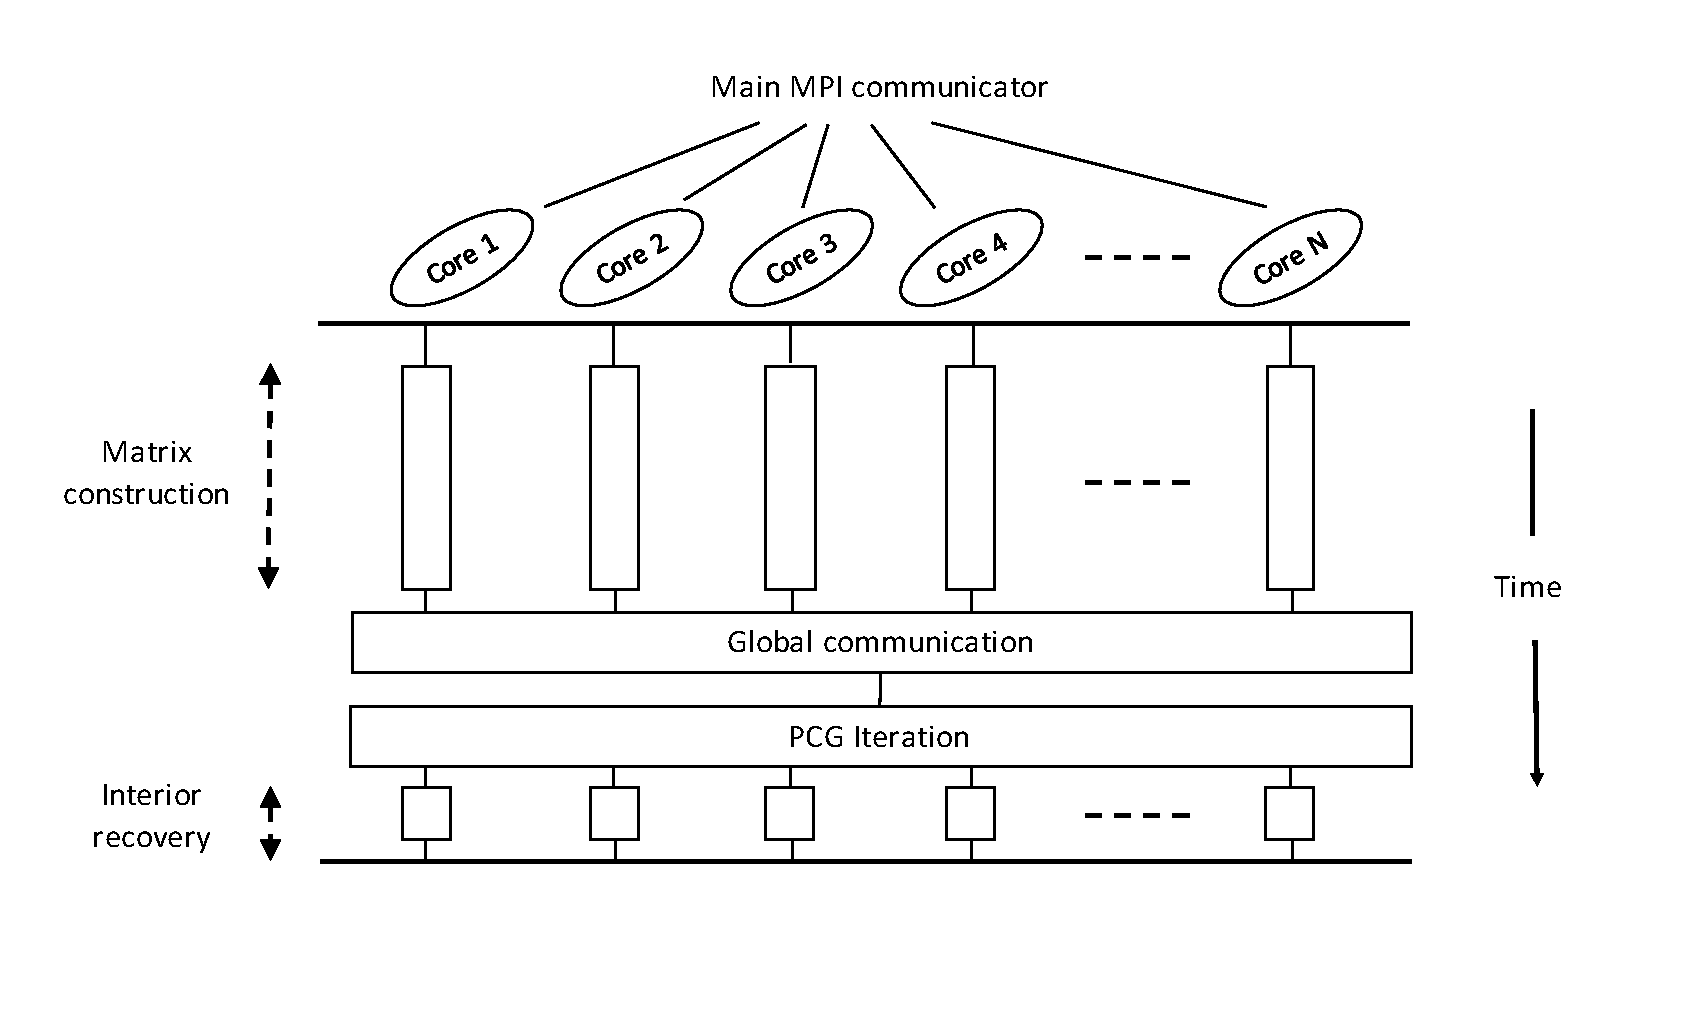
\includegraphics[width=1.0\textwidth]{./pics/mpi_flow.eps}
	\end{tabular}
	\caption{\footnotesize Parallel computing work flow.}\label{fig6: mpi}
\end{figure}
The software has been tested on the George Washington University cluster, ColonialOne, with Xeon E5-2650v2 2.6 GHz 8-core processors with 128 GB of RAM each.

%=================================================
\section{Numerical Results}

\subsection{Poisson Equation}
The WG element can choose different order of basis function in weak gradient equation. Hence, we test the combination order of interior, boundary and weak gradient shape functions. 

The Poisson equation $ -\nabla \cdot (\nabla \mathbf{u}) = \mathbf{f} $ is considered in the test. Let $ \Omega = (0, 1) \times (0, 1) $, $ a = I $, and $ f $ are chosen such that the exact solution is $ u = sin(\pi x) sin(\pi y) $

We choose different weak Galerkin elements for validating our WG-BDDC numerical scheme. The unit square is firstly decomposed into $ N \times N $ subdomains as the coarse mesh with length $ H = 1 / N $. In every subdomain, all elements are further triangulated into a $ 2 n \times n $ triangles, and the finite mesh has the size $ h = 1/(N\times n) $. The preconditioned system is solved by the PCG solver. In every iteration, the $ L^2- $norm of the residual is reduced by a factor of $ 10^{-6} $. The $ L^{2} $ error is calculated by using the equation $ e_{L^{2}} = \sqrt{\sum_{k = 1}^{n} (u - u_{t})^{2} } $

\begin{table}[h]
	\setlength{\tabcolsep}{2pt} {
		\caption{ Performance with $P_{k}P_{k-1}P_{k-1}^2$.}
		\label{Tab:case1_PkPk-1Pk-1}
		\vspace{-5pt}
		\begin{center}
			%	\scalebox{0.6}{
			\begin{tabular}{c|cccc|c|cccc}
				\hline
				\multirow{2}{*}{\#sub} &\multicolumn{4}{c|}{$k=1$ and $H/h=8$} &\multirow{2}{*}{$H/h$} &\multicolumn{4}{c}{$k=1$ and \#sub=64}\\ 
				& Cond.   & Iter. &$L^2$-error & $ O $ & & Cond.   & Iter. &$L^2$-error &$ O $ \\
				\hline
				$4\times 4$     &2.217 &5 &1.6013e-3 &- &4   &1.722 &7   &1.6013e-3 & -\\
				$8\times 8$     &2.390 &9 &3.9939e-4 & 2.0 &8   &2.390 &9   &3.9939e-4& 2.0\\
				$16\times 16$ &2.335 &8 &9.9789e-5 & 2.0 &16 &3.245 &10 &9.9789e-5 & 2.0\\
				$32\times 32$ &2.325 &8 &2.4944e-5 & 2.0 &32 &4.239 &11 &2.4944e-5 & 2.0 \\
				\hline
				\multirow{2}{*}{\#sub} &\multicolumn{4}{c|}{$k=2$ and $H/h=8$} &\multirow{2}{*}{$H/h$} &\multicolumn{4}{c}{$k=2$ and \#sub=64}\\ 
				& Cond.   & Iter. &$L^2$-error & $ O $ & & Cond.   & Iter. &$L^2$-error & $ O $  \\
				\hline
				$4\times 4$    &3.528 & 8  &7.1456e-5 & -  &4   &2.900 &10 &7.1456e-5 & - \\
				$8\times 8$    &3.803 &10 &8.9214e-6 & 3.0 &8   &3.803 &10 &8.9214e-6 & 3.0 \\
				$16\times 16$&3.768 &10 &1.1150e-6 & 3.0 &16 &4.957 &12 &1.1150e-6 & 3.0 \\
				$32\times 32$&3.758 &10 &1.3938e-7 & 3.0 &32 &6.218 &13 &1.3938e-7 & 3.0\\
				\hline
			\end{tabular}
			%	}
		\end{center} }
	\end{table}
	
	The first test is implemented for weak Galerkin element $ u_0 \in P_k, u_b \in P_{k - 1} $, and $ \nabla_w u \in P_{k - 1} $. \ref{Tab:case1_PkPk-1Pk-1} shows the condition number of lanczos matrix and the iteration number in PCG solver. From the \ref{Tab:case1_PkPk-1Pk-1}, we can see that the condition number is independent of the number of subdomain, while it depends on $ H/h $ as $ (1 + log(\frac{H}{h}))^{2} $. Meanwhile, the communication between each adjacent subdomain does not introduce any error to the results. With the increasing of number of subdomains, we obtain stable second and third order of results. The iteration number of global matrix increases slowly to the number of subdomains.
	
	
	\begin{table}[h]
		\small
		\setlength{\tabcolsep}{1pt} {
			\caption{ Performance with $P_{k}P_{k}P_{k-1}^2$.}
			\label{Tab:case1_PkPkPk-1}
			\begin{center}
				%\scalebox{0.8}{
				\begin{tabular}{c|cccc|c|cccc}
					\hline
					\multirow{2}{*}{\#sub} &\multicolumn{4}{c|}{$k=1$ and $H/h=8$} &\multirow{2}{*}{$H/h$} &\multicolumn{4}{c}{$k=1$ and \#sub=64}\\ 
					& Cond.   & Iter. &$L^2$-error & $O1$ & & Cond.   & Iter. &$L^2$-error & $O$\\
					\hline
					$4\times 4$ & 2.451 & 7 & 1.0109e-3 & - &$4$ &1.968 &8 &1.0109e-3 &-\\
					$8\times 8$ &2.648 &9 &2.5117e-4 &	2.0  &8 &2.648 &9 &2.5117e-4 &2.0 \\
					$16\times 16$ &2.629 &9 &	6.2696e-5 &2.0  &16 &3.529 &10 &6.2696e-5 &2.0\\
					$32\times 32$ &2.617 &9 &1.5668e-5 &2.0  &32 &4.619 &12 &1.5668e-5 &2.0\\
					\hline
					\multirow{2}{*}{\#sub} &\multicolumn{4}{c|}{$k=2$ and $H/h=8$} &\multirow{2}{*}{$H/h$} &\multicolumn{4}{c}{$k=2$ and \#sub=64}\\ 
					& Cond.   & Iter. &$L^2$-error &  $\lambda_1$ & & Cond.   & Iter. &$L^2$-error & $\lambda_1$\\
					\hline
					$4\times 4$ & 3.805 &8 &6.6333e-5  &- &4 &3.926 &11 &6.6333e-5  &-\\
					$8\times 8$ & 4.003 &12 &8.2709e-6  & 3.0 &8 &4.003 &12 &8.2709e-6  &3.0 \\
					$16\times 16$ &3.943 &12 &1.0334e-6  &3.0 &16 &5.084 &13 &1.0334e-6  &3.0\\
					$32\times 32$ &3.917 &12 &1.2917e-7  &3.0 &32 &6.329 &13 &1.2918e-7  &3.0\\
					\hline
				\end{tabular}
				%	}
			\end{center} }
		\end{table}
		
		The second test is the weak Galerkin element with order $ u_{0} \in P_{k} $, $ u_{b} \in P_{k} $ and $ \nabla_{w} \in P_{k - 1} $. The condition number has the identical pattern of the theoretical convergence rate. Comparing with the first example, we can find the convergence rates and accuracy have optimal agreement to the degree of polynomial in $ u_{0} $. The parallel scalability is up to 1,000 processors.
		
		\begin{table}[h]
			\small
			\vspace{-10pt}
			\setlength{\tabcolsep}{1pt} {
				\caption{Case 1: Performance with $P_{k}P_{k}P_{k}^2$.}
				\label{Tab:case1_PkPkPk}
				\vspace{-5pt}
				\begin{center}
					%\scalebox{0.8}{
					\begin{tabular}{c|cccc|c|cccc}
						\hline
						\multirow{2}{*}{\#sub} &\multicolumn{4}{c|}{$k=1$ and $H/h=8$} &\multirow{2}{*}{$H/h$} &\multicolumn{4}{c}{$k=1$ and \#sub=64}\\ 
						& Cond.   & Iter. &$L^2$-error & $O$  & & Cond.   & Iter. &$L^2$-error & $O$ \\
						\hline
						$4\times 4$     &3.671 & 8  &2.1451e-4 &- &4   &3.024 &10 &2.1451e-4 &- \\
						$8\times 8$     &3.965 &10 &5.2129e-5 &2.0  &8   &3.965 &10 &5.2129e-5 &2.0 \\
						$16\times 16$ &3.934 &10 &1.2937e-5 &2.0  &16 &5.153 &12 &1.2937e-5 &2.0 \\
						$32\times 32$ &3.922 &10 &3.2281e-6 &2.0  &32 &6.472 &14 &3.2281e-6 &2.0 \\
						\hline	
						\multirow{2}{*}{\#sub} &\multicolumn{4}{c|}{$k=2$ and $H/h=8$} &\multirow{2}{*}{$H/h$} &\multicolumn{4}{c}{$k=2$ and \#sub=64}\\ 
						& Cond.   & Iter. &$L^2$-error & $O$ & & Cond.   & Iter. &$L^2$-error & $O$ \\
						\hline
						$4\times 4$     &4.620 &8   &6.7627e-6 &-  & 4  &3.859 &11 &6.7628e-6 &- \\
						$8\times 8$     &4.987 &12 &7.8998e-7 &3.0  &8   &4.987 &12 &7.8998e-7 &3.0 \\
						$16\times 16$ &4.921 &12 &9.6925e-8 &3.0  &16 &6.235 &13 &9.6931e-8 &3.0 \\
						$32\times 32$ &4.901 &12 &1.2058e-8 &3.0  &32 &7.673 &15 &1.2060e-8 &3.0 \\
						\hline
					\end{tabular}
					%}
				\end{center} }
			\end{table}
			
			In the third test, we implement the weak Galerkin element $ u_{0} \in P_{k} $, $ u_{b} \in P_{k} $ and $ \nabla_{w} u \in P_{k} $. The $ P_k P_k P_k^2 $ element deliveries the most accurate result among all three types of element. The reason is that all three shape functions of interior variable, boundary variable and weak gradient have the same order. 
			
			
			\subsection{Linear Elastic Equation}
			
			We consider the linear elastic equation (1) in the square domain $ \Omega = (0, 1)^{2} $ which is decomposed into uniform square subdomains with size $ H $. For each subdomain, it is partitioned into uniform quadrilateral mesh with size $ h $. The exact solution is given by
			\begin{equation}
			u = \begin{pmatrix}
			sin(2\pi x)sin(2\pi y) \\ 1
			\end{pmatrix}
			\end{equation}
			
			\begin{table}[h]
				\small
				\vspace{-10pt}
				\setlength{\tabcolsep}{1pt} {
					\caption{Case 1: Performance with $P_{1}P_{1}$, $ \lambda = 1, \mu = 0.5 $}
					\label{Tab:case1_PkPkPk linear}
					\vspace{-5pt}
					\begin{center}
						%\scalebox{0.8}{
						\begin{tabular}{c|cccc|c|cccc}
							\hline
							\multirow{2}{*}{\#sub} &\multicolumn{4}{c|}{ $H/h=8$} &\multirow{2}{*}{$H/h$} &\multicolumn{4}{c}{$k=1$ and \#sub=64}\\ 
							& Cond.   & Iter. &$L_{Max}$-error & $O$& & Cond.   & Iter. &$L^2$-error & $O$ \\
							
							\hline
							$2\times 2$     & 2.281 & 8   & 8.484e-2 & - & 4   & 2.212 &11 & 2.993e-1 &- \\
							$4\times 4$     &3.922 &12 &2.1787e-2 & 1.96 & 8   & 3.069 &12 & 8.567e-2 & 1.9  \\
							$8\times 8$  & 4.895 &17 &5.4706e-3 & 1.99 & 16   & 4.143 &13 & 2.217e-2 & 2.0 \\
							$16\times 16$ &5.238&17 &1.3675e-3 & 2.00 & 32   & 5.437 &15 & 5.575e-3 & 2.0 \\
							\hline	
						\end{tabular}
						%	}
					\end{center} }
				\end{table}
				
				We test the performance of WG-BDDC on cluster and present the speedup figure which indicates the superlinear acceleration and good scalability. 
				
				\begin{figure}[h]
					\centering
					\begin{tabular}{cc}
						\includegraphics[width=0.6\textwidth]{./pics/p1time.eps} 
					\end{tabular}
					\caption{\footnotesize The running time .vs. number of processors.}\label{fig6: time}
				\end{figure}
				
				
					\begin{figure}[h]
						\centering
						\begin{tabular}{cc}
							 \includegraphics[width=0.6\textwidth]{./pics/p1speed.eps}
						\end{tabular}
						\caption{\footnotesize The speedup .vs. number of processors.}\label{fig6: time}
					\end{figure}
				
				The blue dot line called WGDD represents WG-BDDC method. we can see from the above figures that the superlinear speedup is captured within the increasing of the number of subdomains. The main concern for BDDC method is that the balance between global matrix, the preconditioner, and the local matrices. It is important to estimate the size of preconditioner and choose proper number of processors.
				
				
	we report a novel parallel computing method. This method integrated the newly developed weak Galerkin finite element method with balancing domain decomposition with constraints. The MPI library is set up for information communication between each processor. The optimal convergence rate and promising scalability of this WG-BDDC method are observed.
	
	To this method, it is convenient to implement high order element. We have multiple choices on interior, boundary and gradient basis functions which is an obvious flexibility to numerical calculation. We can design the element type based on our need. From the optimal convergence rate, we can conclude that this method is robust and highly compatible to different element orders.
	
	For the results, all test cases have well bounded condition numbers for the global matrices which fits our initial assumption properly. Meanwhile, the superlinear feature from the speedup graph is also in favor of high performance computing. This is the first attempt to introduce weak Galerkin to engineering purpose implementation. The optimal performance on parallel computing indicates a promising future of this method.

\chapter{Numerical Simulations of Stenotic Flow}

Peripheral arterial occlusive diseases, especially in femoral arteries are commonly seen by clinical doctors in the U.S.\cite{malinow1989prevalence, boger1997biochemical, hooi2001incidence}. These patients may have critical stenoses or multiple sequential moderate stenoses. The current clinical practice usually recommends simple balloon angioplasty\cite{duncan1995simple} to treat critical stenotic lesion, i.e. $ > 60 \% $ luminal area reduction. However, it is a difficult process for the doctors to make a decision on whether or not to treat multiple sequential moderate stenoses using the stent or balloon angioplasty. This is partially because of the lack of methods to measure how these multiple stenoses affect their downstream blood flow. The scientific study of fluid dynamics associated with multiple stenoses is far less than that of a single stenosis. To assist on making clinical decision for treating multiple stenoses, a quantitative approach, for instance, the computational fluid dynamics (CFD) \cite{ferziger1997computational} method is very much needed. In this study,  we present a high-fidelity CFD simulations of the blood flow in the stenotic arteries using idealized geometries. We solve unsteady incompressible Navier-Stokes equations\cite{temam1984navier} using unstructured meshes with all hexahedral elements. The upstream flow condition is prescribed which gives a Reynolds number of 500. Our simulations results reveal several new discoveries of fluid dynamics in these multiple stenoses considering a range of different geometric parameters.

\section{Background}

Peripheral arterial occlusive disease are the major cause of amputation in the U.S. as they are prevalent among smokers, diabetics, hypertensives, and patients with dyslipidemia. Nowadays, since the disease can be visualized as areas of stenosis or occlusion on a diagnostic arteriogram, simple balloon angioplasty with or without stenting is usually recommended for treating critical stenotic lesions, i.e. $ > 60\% $ (by area) luminal reduction. However, the clinical decision is rather difficult on whether or not to treat subcritical stenotic lesions, i.e., $ < 50\% $ luminal reduction, in particular, multiple sequential moderate stenoses. The risks of routine ballloon angioplasty/stenting include intimal injury-induced acute arterial thrombosis or restenosis\cite{holmes1984restenosis} from neointimal hyperplasia\cite{kornowski1998stent}, etc. These risks led to the difficulty of telling the benefits of treating mildly stenotic lesions using routine clinical treatment. Meanwhile, there is no existing method to measure the effects of multiple sequential moderate stenoses on blood flow in the part of the artery that is downstream of the stenotic lesions. The closest measurement that correlated with change in blood flow is the change in arterial pressures. If the arterial pressure drop across the stenoses is greater than the clinical threshold (20-30mmHg) \cite{meuwissen2002hyperemic}, the lesions are considered physiologically significant enough to favor treatment. However, it's clinically very difficult to quantify. Consequently, CFD simulation is a helpful supplement for the stenosis study.

\begin{figure}[H]
	\centering
	\begin{tabular}{c}
		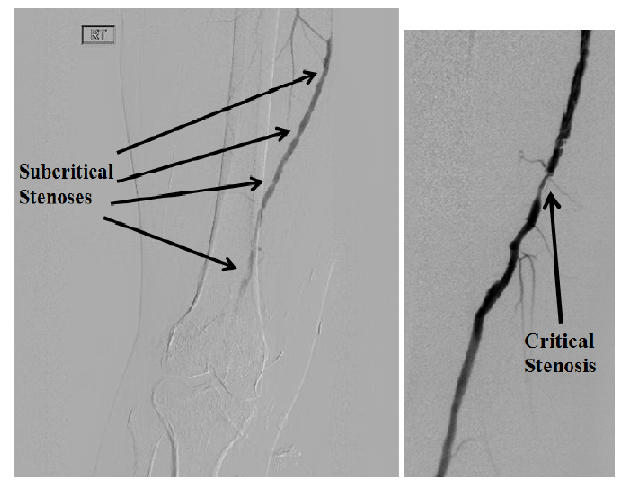
\includegraphics[width=0.6\textwidth]{./pics/photo.png}
	\end{tabular}
	\caption{\footnotesize Contrast of subcritical and critical stenoses.}
\end{figure}

A good amount of investigation have been addressed on pressure drop across single stenosis from both experimental and analytical perspective\cite{Ojha,Varghese,Young&Tsai,Young&Cholvin,Seeley&Young,Varghese&Frankel}. At the beginning, investigators derived empirical function from conservation equations with the experimental coefficients for both steady and pulsatile flow condition. The empirical function is a simplified estimation for pressure drop across single stenosis. A series computational simulations and experiments rendered the details of flow field across constriction. 
Flanigan et al\cite{flanigan1977multiple} conducted a series of experiments and proposed non-linear relationship between number of applied stenoses and pressure drop across the stenoses.
Bertolotti et al\cite{bertolotti2006influence}, using finite element method, simulated the pressure drop and velocity field through two adjacent stenoses at very low Reynolds number.

We have implemented an efficient in-house CFD package which has the capability to simulate more complex 3D geometries. This paper reports a range of parametric studies including varying the number of stenoses, the narrowing degrees, the shapes, and streamwise spacing. The object is providing to doctors an accessible effective approach which can predict the pressure and the velocity field of stenotic arteries. These stenotic arteries consist of patient-specific geometries which are challenging to define computationally. These arteries are typically simplified as axisymmetric constriction in straight tubes. The 3D computational domain is represented by unstructured meshes with all hexahedral cells. An efficient pressure-based Finite Volume Method(FVM)\cite{LiangFVM} was implemented to solve these equations. Our simulations include computational geometries with a wide range of narrowing degrees of stenoses, from $ 40\% $ to $ 80\% $ luminal area reduction. The number of stenoses ranges from $ 1 $ to $ 7 $. Several different spatial intervals were considered between adjacent stenoses.
%=========================================

\section{Numerical Method}

The unsteady incompressible Navier-Stokes equations, describing the conservation of mass and momentum in the computational region, are discretized using a second-order central differencing scheme in space and a Crank-Nicolson\cite{briley1977solution} method in time. 
The pressure and velocity are stored in cell centers using the collocated method.
Pressure-velocity coupling is dealt by a Rhie-Chow interpolation method\cite{Rhie} and a PISO algorithm for pressure correction\cite{Issa}.

Mass conservation and Navier-Stokes equations as following:s

\begin{equation}
\frac{\partial u_{i}}{\partial x_{i}} = 0,
\end{equation}

\begin{equation}
\frac{\partial u_{i}}{\partial t} + \frac{\partial u_{i} \partial u_{j}}{\partial x_{j}} = -\frac{1}{\rho} \frac{P}{\partial x_{i}} - \frac{\partial \tau_{ij}}{\partial x_{j}} + \nu \frac{\partial^{2} u_{i}}{\partial x_{j} \partial x_{i}},
\end{equation}

where the index $ i = 1, 2, 3 $ represents three directions in the Cartesian coordinate system, $ P $ is the pressure, $ \rho $ is density, and $ \nu $ is kinematic viscosity.

\section{Geometry and Condition}

\subsection{Geometry}

The geometry of stenoses along peripheral artery is complex and irregular. A symmetrical constriction in a straight cylindrical tube is a proper idealization method to simplify the complicated problem\cite{Long}. The shape of the stenoses are optimized by using third order degree polynomial. In the following figure shows three sequential $ 50\% $ degree stenoses along the straight vessel.

\begin{figure}[H]
	\centering
	\begin{tabular}{c}
		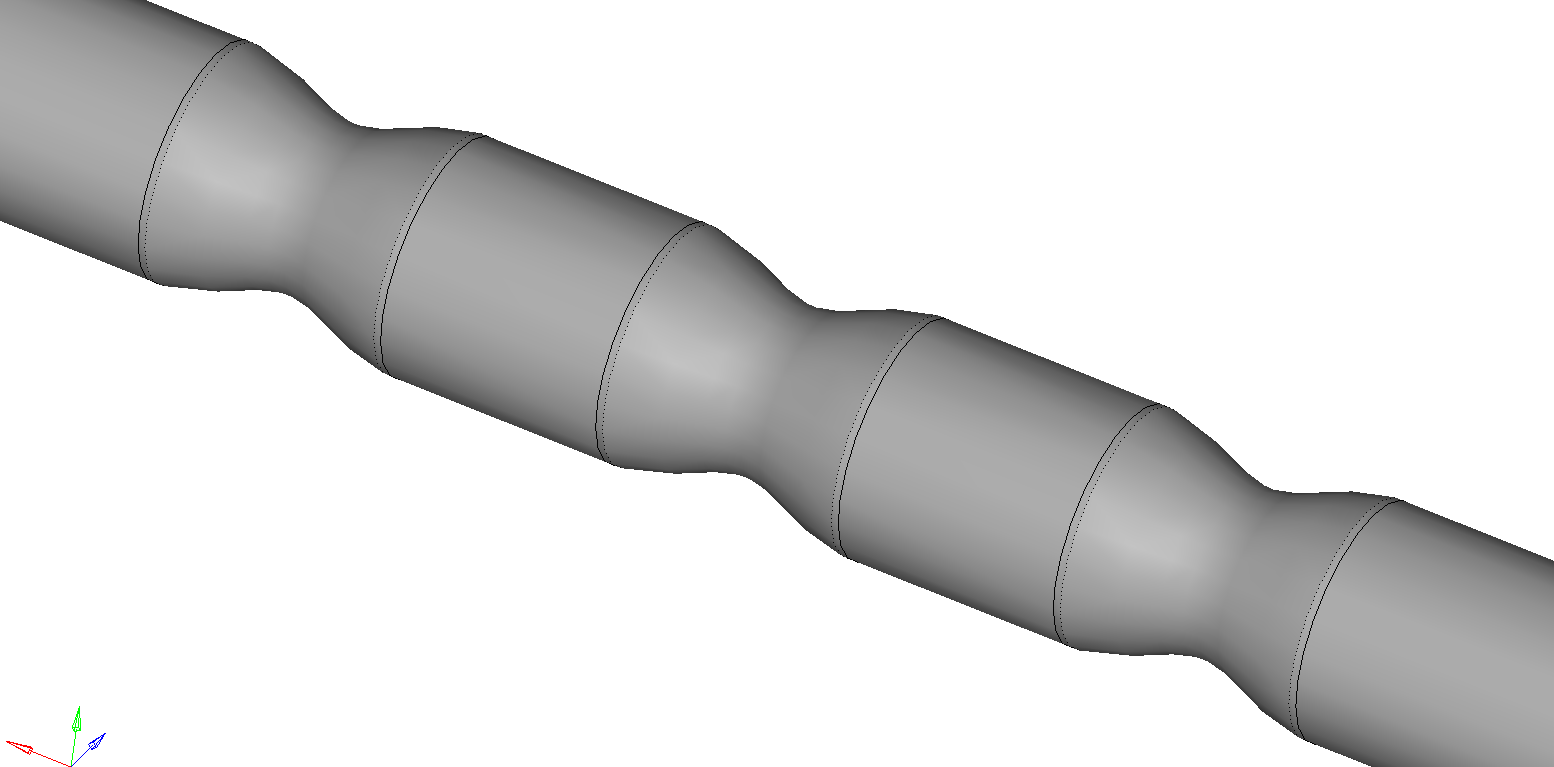
\includegraphics[width=0.6\textwidth]{./pics/geom.png}
	\end{tabular}
	\caption{\footnotesize Geometry of sequential stenoses.}
\end{figure}

\subsection{Mesh}
We implement unstructured hexahedral meshes for idealized stenoses geometry. Internal mesh is total unstructured as the following figure. Moreover, we impose flour boundary layers along the surrounding wall for more accurate prediction of boundary flow.

\begin{figure}[H]
	\centering
	\begin{tabular}{cc}
		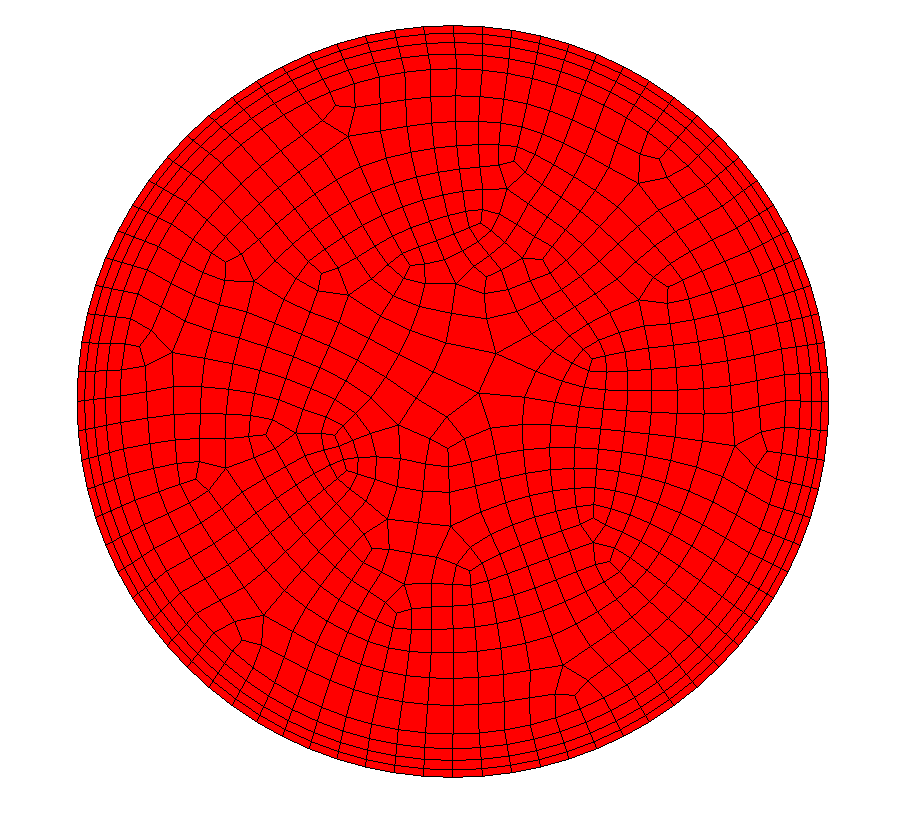
\includegraphics[width=0.3\textwidth]{./pics/mesh1.png} & 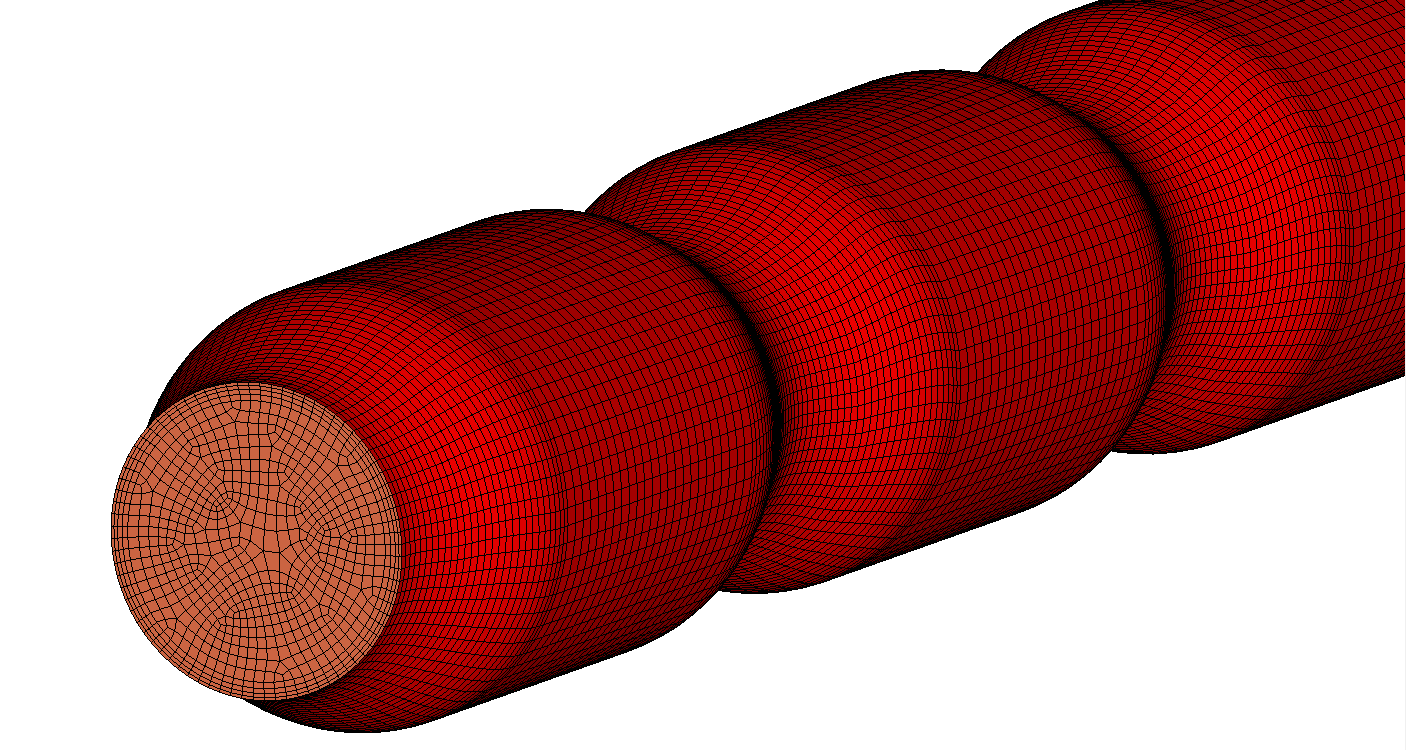
\includegraphics[width=0.6\textwidth]{./pics/mesh7.png}
	\end{tabular}
	\caption{\footnotesize Cross-sectional view of hexahedral meshes.}
\end{figure}

To better analyze the flow cross the stenotic area, we refine the longitudinal mesh across the stnosis. We increase the number of layers along x-axis direction for a better mesh adaptation of stenosis curve.

\begin{figure}[H]
	\centering
	\begin{tabular}{cc}
		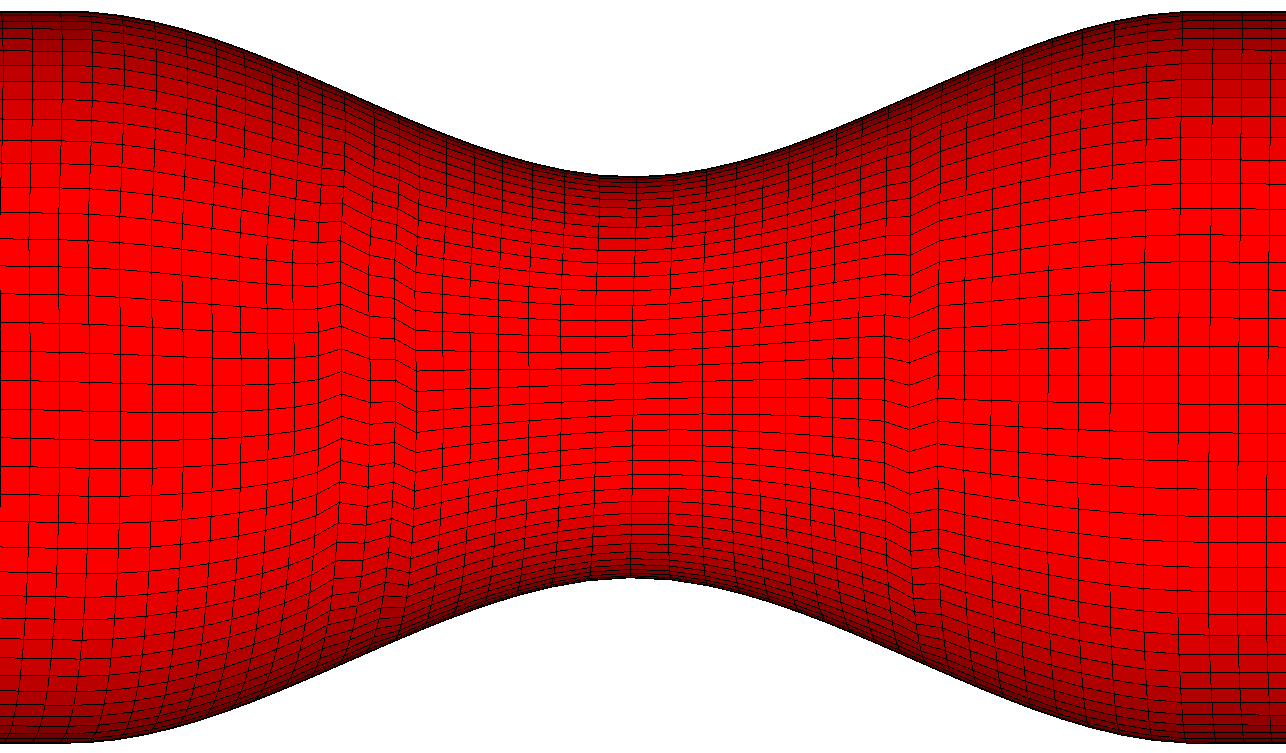
\includegraphics[width=0.4\textwidth]{./pics/refine1.png} & 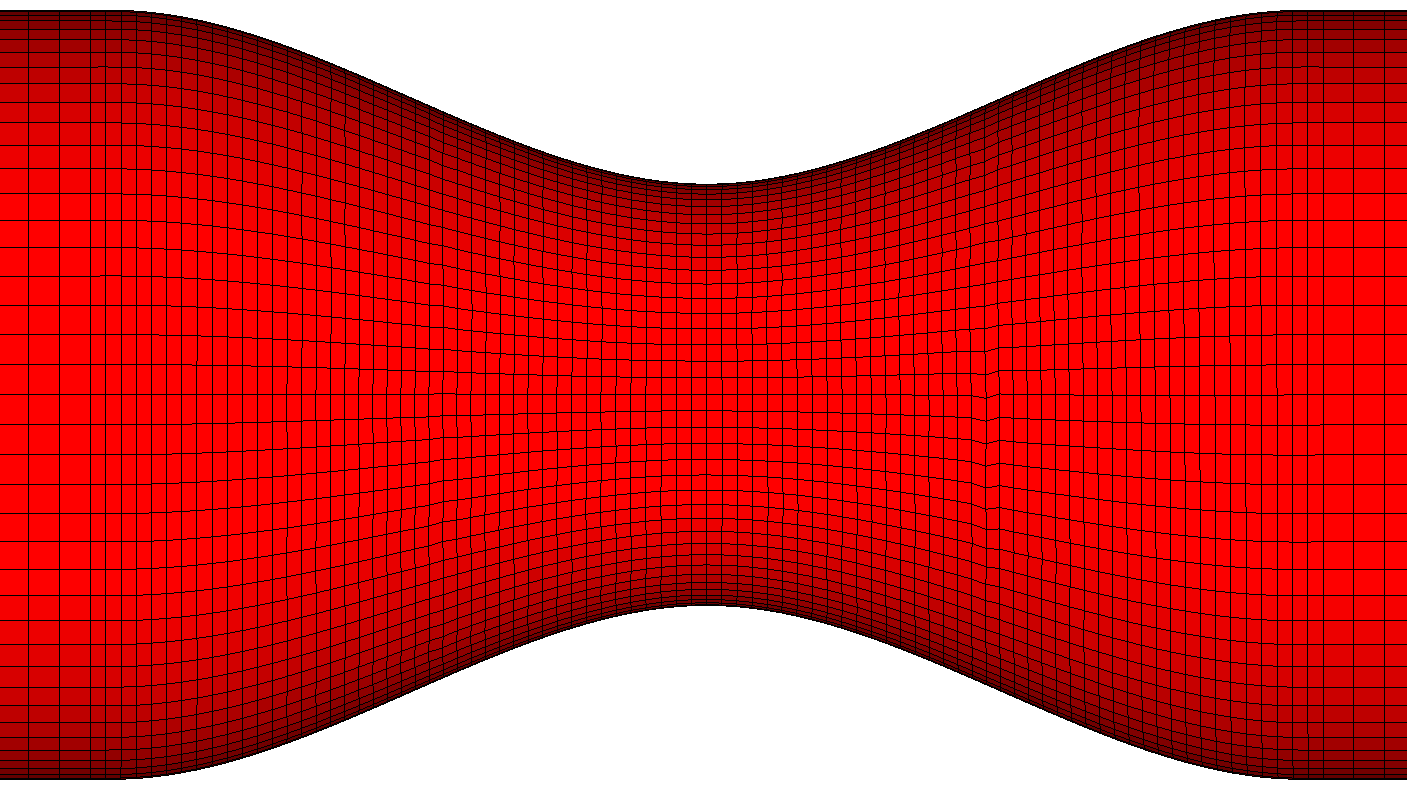
\includegraphics[width=0.4\textwidth]{./pics/refine2.png}
	\end{tabular}
	\caption{\footnotesize Mesh refinement for stenotic area.}
\end{figure}

\subsection{Dimensionless wall distance}

The transition flow happens when the flow passing critical (i.e. $ >70\% $) stenosis. The dimensionless wall distance is defined as:

\begin{equation}
y^{+} = \frac{u_{*} y}{\nu}
\end{equation}

where $u_*$ is the friction velocity at nearest wall, $y$ is the distance to the nearest wall,$\nu$ is the local. kinematic viscosity of fluid. 
We control the $y^+ \le 1$ after refine the mesh with boundary layers. This condition insure that viscosity plays an important role rather than advection.

\subsection{Conditions}

	\begin{table}[!h]
		\caption{ Simulation condition parameters.}
		\vspace{-5pt}
		\begin{center}
			%	\scalebox{0.6}{
			\begin{tabular}{|c|c|}
				\hline
				\textbf{Variable} &\textbf{Value}\\
				\hline
				Stream wise length & 30D\\
				\hline
				Reference mesh points & 720,000\\
				\hline
				Reynolds number for inlet & 500\\
				\hline
				Maximum of CFL number & 0.79\\
				\hline
			\end{tabular}
			%	}
		\end{center} 
	\end{table}

	We implement parabolic velocity profile as inlet boundary condition, Neumann condition as the outlet boundary condition.
	We impose no-slip boundary condition on rigid and non-porous walls.
	The fluid is incompressible Newtonian with same mean Reynolds number as blood in peripheral arteries ${Re}_{mean} = 500$.
	The entrance length of 6 diameters is sufficient for flow development.

%=========================================

\section{Verification}
\subsection{Straight vessel test}
First of all, we implement a simulation on a straight tube without any constriction.
For the straight tube, we use the following analytical function to calculate the pressure drop
\begin{equation}
\Delta P  = \frac{128 \mu l Q}{\pi D^4}
\end{equation} 
We compare the pressure drop between simulation results and analytical solution. The error is less than $0.25$\%.

\begin{table}[h]
	\caption{ Straight vessel test results.}
	\vspace{-5pt}
	\begin{center}
		%	\scalebox{0.6}{
		\begin{tabular}{|c|c|}
			\hline
			\textbf{Cases} &\textbf{Value}\\
			\hline
			Simulation result & 408.6 \\
			\hline
			Analytical solution & 409.9 \\
			\hline
			Error & $<0.25$\% \\
			\hline
		\end{tabular}
		%	}
	\end{center} 
\end{table}

For the following cases, we use the value of pressure drop through the straight tube as a reference bar.
All the parameters including absolute and stream-wise pressure drop are plotted over the reference value.
The coordinate information are plotted over the diameter.
Then all the parameters on the following figures are dimensionless.

\subsection{Resolution independence test}

In this section, we present the results of same geometry with two different mesh resolutions.
The test cases are straight tubes with 10 diameters long. 

\begin{figure}[H]
	\centering
	\begin{tabular}{cc}
		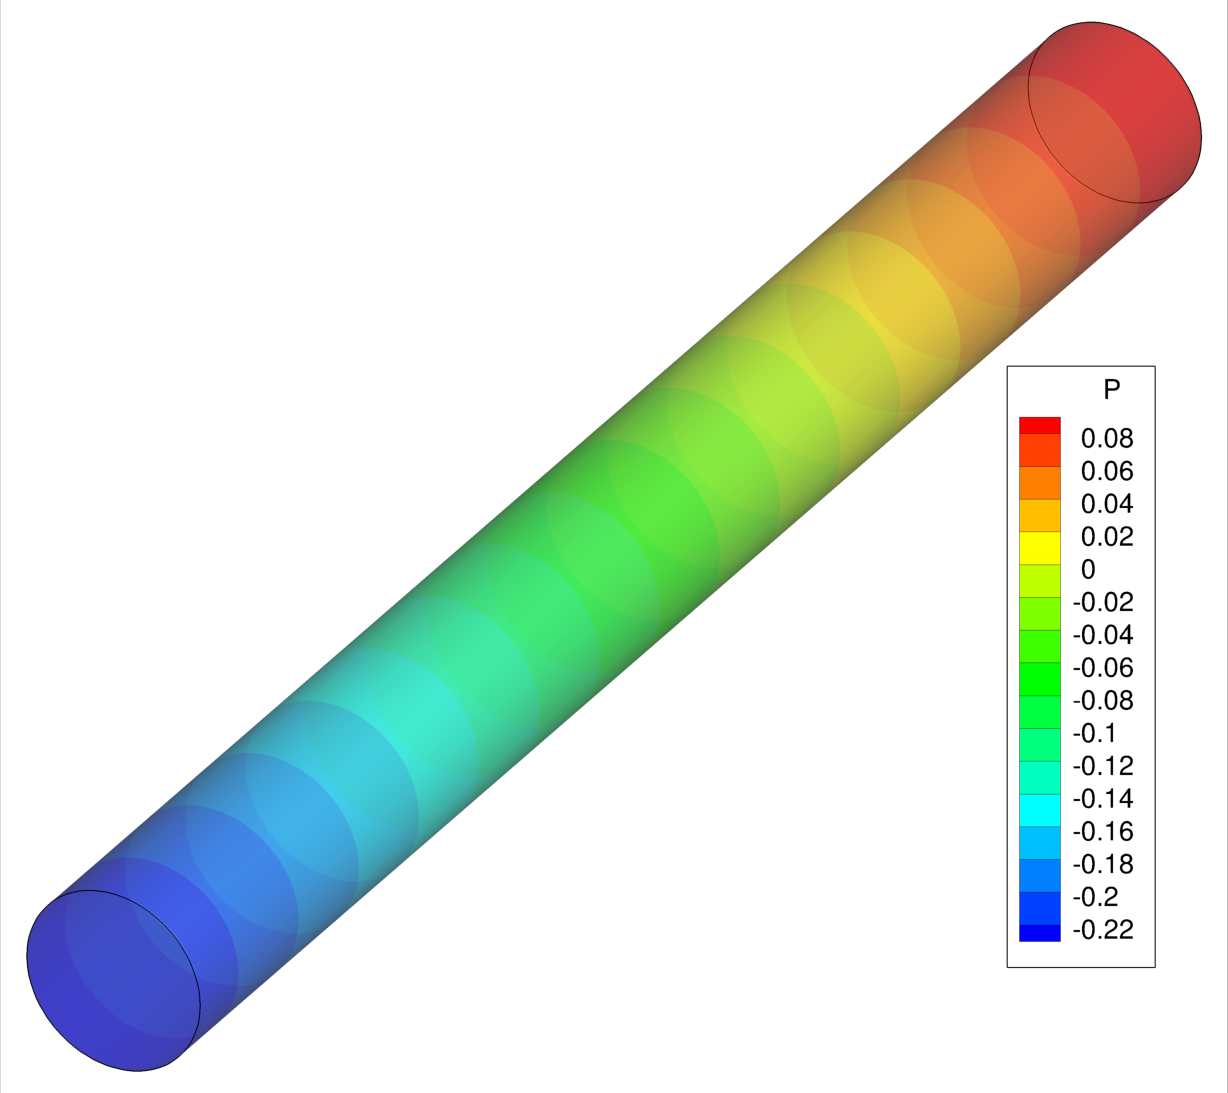
\includegraphics[width=0.4\textwidth]{./pics/plotbio.png} & 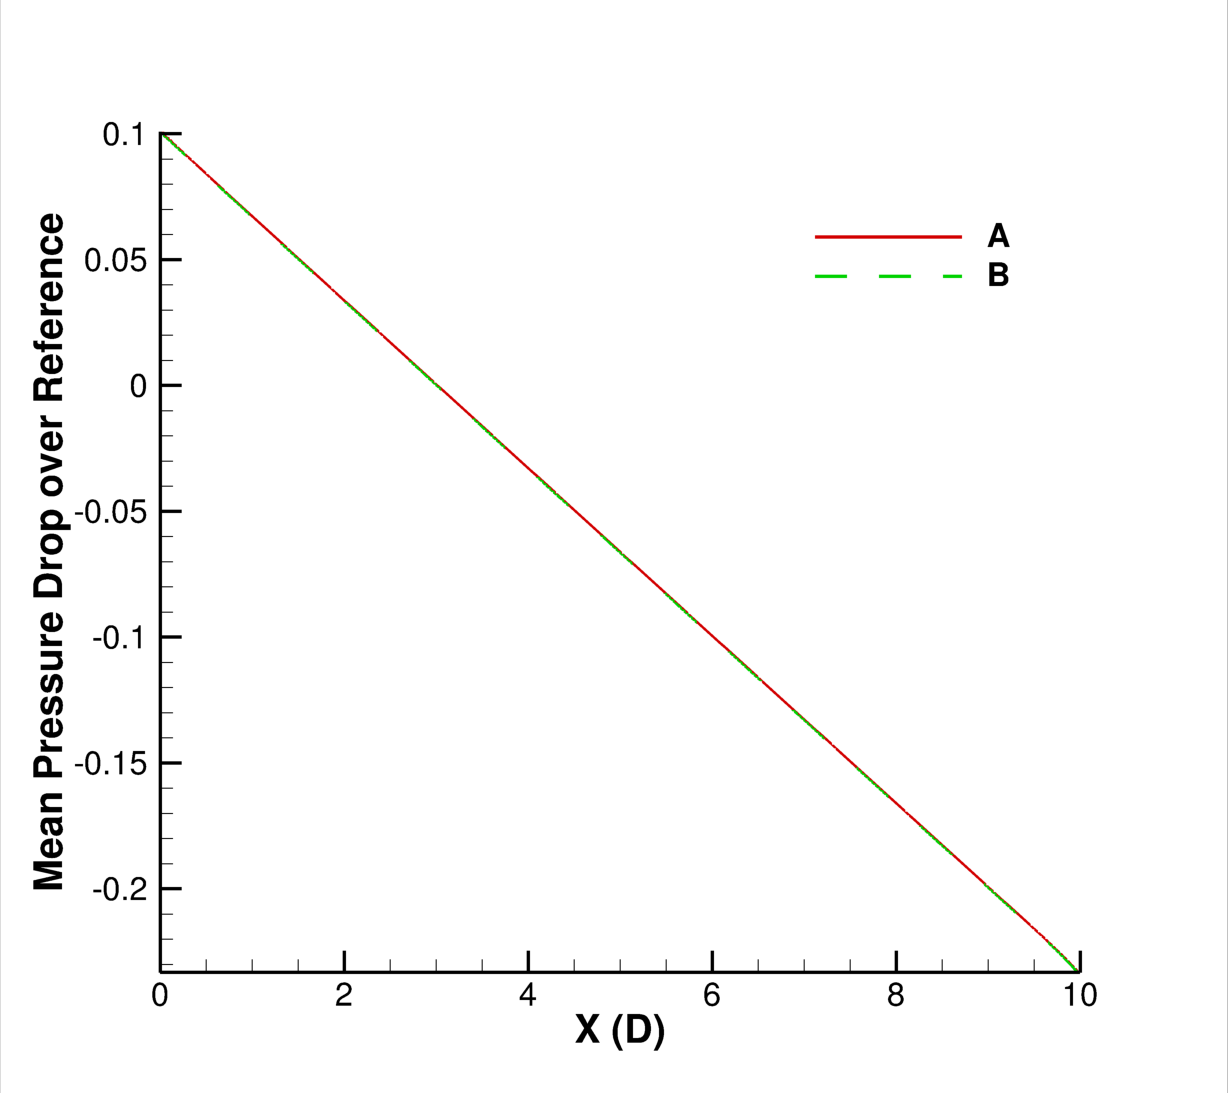
\includegraphics[width=0.4\textwidth]{./pics/resolution.png}
	\end{tabular}
	\caption{\footnotesize Resolution independence test plot and results comparison.}
\end{figure}

The reference mesh grids number of case A is 240000. The resolution of case A is as same as the rest simulations of this paper. We double the number of mesh grid along the longitudinal direction. The finer mesh case B has 480000 grid points. Then we simulate both cases with our solver and compare the results with analytical solution.

\begin{table}[h]
	\caption{Resolution independence test results.}
	\vspace{-5pt}
	\begin{center}
		%	\scalebox{0.6}{
	\begin{tabular}{|c|c|c|}
		\hline
		\textbf{Cases} &\textbf{Value} & \textbf{Error}\\
		\hline
		A & 136.946 & $<0.57\%$\\
		\hline
		B & 137.211 & $<0.76\%$\\
		\hline
		Analytical & 136.169 & 0 \\
		\hline
	\end{tabular}
		%	}
	\end{center} 
\end{table}

The error of both cases are very low and neglectable. The resolution of case A is same as all the simulations in this paper. From this comparison we can conclude that our resolution is sufficient for pipe-flow study. It is a good compromise on accuracy and efficiency of simulations.

\subsection{Verification Established Empirical Solution}

In Young and Tsai\cite{Young&Tsai} study, the major factors controlling the pressure drop, $\triangle p$, across a single stenosis can be estimated from the following empirical equation:

\begin{equation}
\triangle p = \frac{K_v \mu}{D} U + \frac{K_t}{2}(\frac{A_0}{A_1} -1)^2 \rho \lvert U \rvert U %+ K_u \rho L \frac{dU}{dt}
\end{equation}
where $A_0$ = area of the unobstructed tube, $A_1$ = minimum cross-sectional area of the stenosis,
$D$ = unobstructed tube, $K_v$ and $K_t$ = experimentally determined coefficients, 
$L$ = length over which the pressure drop is measured, $U$ = instantaneous velocity in the unstructed tube,
$\rho$ = blood flow density, and $\mu$ = blood flow viscosity. 

Young et al\cite{Young&Cholvin} pointed out that $K_v$ and $K_t$ are dependent on stenosis geometry and narrowing degree.
$K_v$ can be approximated from steady-flow tests with streamlined plug as single stenosis.
The values of $K_v$ in our simulations range from 630 to 2300 of the stenosis narrowing degree from 40\% to 80\% area reduction.
Another empirical coefficient, $K_u$, gives the best fit of data is 1.2.

\begin{figure}[H]
	\centering
	\begin{tabular}{c}
		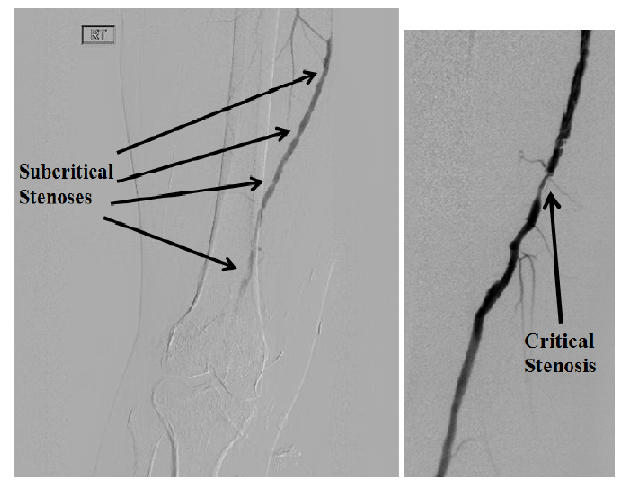
\includegraphics[width=0.6\textwidth]{./pics/photo.png}
	\end{tabular}
	\caption{\footnotesize Contrast of subcritical and critical stenoses.}
\end{figure}
%=========================================

\section{Results}

To analyze the hemodynamic effect caused by variant stenoses, we introduced two key parameters which describe the pressure field through stenotic artery. 
The first one is the  stream-wise pressure drop which indicates the pressure difference from the inlet to the outflow area through the whole arterial domain.  
It describes the hemodynamic effect of stenoses among the entire flow domain. The doctors currently are using it as a prime clinical indicator to evaluate blood supplement to downstream bodies. Doctors are using this parameter to make the treatment decision.
The other one is the absolute pressure drop which means the pressure difference between the maximum pressure value (at the inflow area) and minimum pressure value (at the last post-stenotic area). 
This parameter demonstrates the stenotic lesion induces a low pressure field concentrated at the post-stenotic area. 
The certain low pressure flow area is a potential serious damage source to the blood vessels which may leads to restenosis after the treatment. 




\chapter{Conclusions and Future Work}

\section{Conclusion}

In this dissertation, we have successfully designed a novel parallel computing method for solving linear elasticity problems. This method integrates the newly developed weak Galerkin (WG) finite element method with a balancing domain decomposition with constraints (BDDC). The WG-BDDC method is implemented by using Fortran and MPI libraries. The WG-BDDC method is demonstrated to have optimal order of accuracy and convergence properties for both 2nd- and 3rd- order numerical discretization. This method is also proven to have outstanding scalability with superlinear speedup when the number of processors increases by testing up to 600 processors. The condition numbers of the Lanczos matrix from the global primal problem for all test cases presented in this paper are well bounded demonstrating fast and robust convergence properties.

%In hemodynamic perspective, we designed a study on peripheral arterial disease. Based on the collected data, we proved our following predictions: the post-stenotic flow becomes highly unsteady when the narrow degree is over $ 60\% $ area deduction. More than 3 successive $ 50\% $ stenoses cause more streamwise pressure drop than one single $ 60\% $ stenosis. Moreover, pressure drop introduced by  subcritical stenoses grows linearly as the increasing number of applied stenoses. In conclusion, the cross-sectional area reduction is the main factor which contributes to the total.

\section{Future Work}

The Future Work consists of two major steps: 1) further develop the WG-BDDC scheme for nonlinear elasticity problems, 2) extend the current WG-BDDC to tetrahedron and hexahedron elements and incorporate the IMEX coupling scheme to implement an efficient fluid-structural interaction solver.

The present WG-BDDC method is built on triangular and quadrilateral 2 dimensional elements for solving linear elasticity problems. To solve more complicated real-world problems, the nonlinear elasticity equation and three dimensional geometry model are urgent. Our ultimate goal is to simulate complex real-world engineering problems with our efficient high-order accuracy structural and fluid solver. The IMEX coupling scheme will combine the two independent solvers together and are expected to produce high-fidelity results.

\bibliographystyle{elsarticle}
\bibliography{references}

\end{document}
